% This is the Reed College LaTeX thesis template. Most of the work
% for the document class was done by Sam Noble (SN), as well as this
% template. Later comments etc. by Ben Salzberg (BTS). Additional
% restructuring and APA support by Jess Youngberg (JY).
% Your comments and suggestions are more than welcome; please email
% them to cus@reed.edu
%
% See http://web.reed.edu/cis/help/latex.html for help. There are a
% great bunch of help pages there, with notes on
% getting started, bibtex, etc. Go there and read it if you're not
% already familiar with LaTeX.
%
% Any line that starts with a percent symbol is a comment.
% They won't show up in the document, and are useful for notes
% to yourself and explaining commands.
% Commenting also removes a line from the document;
% very handy for troubleshooting problems. -BTS

% As far as I know, this follows the requirements laid out in
% the 2002-2003 Senior Handbook. Ask a librarian to check the
% document before binding. -SN

%%
%% Preamble
%%
% \documentclass{<something>} must begin each LaTeX document
\documentclass[12pt,twoside]{reedthesis}
% Packages are extensions to the basic LaTeX functions. Whatever you
% want to typeset, there is probably a package out there for it.
% Chemistry (chemtex), screenplays, you name it.
% Check out CTAN to see: http://www.ctan.org/
%%
\usepackage{graphicx,latexsym}
\usepackage{amsmath}
\usepackage{amssymb,amsthm}
\usepackage{longtable,booktabs,setspace}
\usepackage{chemarr} %% Useful for one reaction arrow, useless if you're not a chem major
\usepackage[hyphens]{url}
% Added by CII
\usepackage{hyperref}
\usepackage{lmodern}
% End of CII addition
\usepackage{rotating}

% Next line commented out by CII
%%% \usepackage{natbib}
% Comment out the natbib line above and uncomment the following two lines to use the new 
% biblatex-chicago style, for Chicago A. Also make some changes at the end where the 
% bibliography is included. 
%\usepackage{biblatex-chicago}
%\bibliography{thesis}


% Added by CII (Thanks, Hadley!)
% Use ref for internal links
\renewcommand{\hyperref}[2][???]{\autoref{#1}}
\def\chapterautorefname{Chapter}
\def\sectionautorefname{Section}
\def\subsectionautorefname{Subsection}
% End of CII addition

% Added by CII 
\usepackage{caption}
\captionsetup{width=5in}
% End of CII addition

% \usepackage{times} % other fonts are available like times, bookman, charter, palatino


% To pass between YAML and LaTeX the dollar signs are added by CII
\title{Turnout and Mail Voting in Colorado; or How I Learned to Stop Worrying
and Love Voter Registration Files}
\author{Theodore Dounias}
% The month and year that you submit your FINAL draft TO THE LIBRARY (May or December)
\date{December 2018}
\division{Mathematics and Natural Sciences and History and Social Sciences}
\advisor{Paul Gronke}
%If you have two advisors for some reason, you can use the following
% Uncommented out by CII
\altadvisor{Andrew Bray} 
% End of CII addition

%%% Remember to use the correct department!
\department{Mathematics and Political Science}
% if you're writing a thesis in an interdisciplinary major,
% uncomment the line below and change the text as appropriate.
% check the Senior Handbook if unsure.
%\thedivisionof{The Established Interdisciplinary Committee for}
% if you want the approval page to say "Approved for the Committee",
% uncomment the next line
%\approvedforthe{Committee}

% Added by CII
%%% Copied from knitr
%% maxwidth is the original width if it's less than linewidth
%% otherwise use linewidth (to make sure the graphics do not exceed the margin)
\makeatletter
\def\maxwidth{ %
  \ifdim\Gin@nat@width>\linewidth
    \linewidth
  \else
    \Gin@nat@width
  \fi
}
\makeatother

\renewcommand{\contentsname}{Table of Contents}
% End of CII addition

\setlength{\parskip}{0pt}

% Added by CII

\providecommand{\tightlist}{%
  \setlength{\itemsep}{0pt}\setlength{\parskip}{0pt}}

\Acknowledgements{

}

\Dedication{

}

\Preface{
I started my second attempt at this preface by reading through my
maternal grandfather's eulogy, and then steadily going through what I
could piece together of my family's story. In my bloodline I have
researchers, engineers, teachers, and social scientists, all with
astoundingly different approaches to stemming their curiosity about the
world around them. All of them, though, have in common that they have
fought long and hard for me to have what I do now, in my privilege to
study at Reed College and live a decent, financially secure life, but
also in my ability to determine my future in a democratic state. They
all fought for Greece to be as free as it is today, even though our
elections may often deliver painful results. I find it very fitting that
the way I honor their legacy is by studying the system that they helped
create\footnote{And by also veering wildly away from any of their own
  previous research interests, much to the occasional chagrin of my
  close relatives, and much in the same fashion that they seem to have
  steered clear of their own parents.}. \par Of course, my object of
study is not Greek, but American elections. I made this choice first by
necessity, since the data access and previous literature is
exponentially greater. I soon realized, however, that the puzzles that
US elections present are both generalizable and deeply intriguing. I was
taken in by the complexity of translating the will of the people for the
world's greatest economic and military power into political action and
by how the most initially mundane policy choices could have massive
impacts on representation. As I mention again in my introduction,
democracies are based on procedures as much as principles, and I am now
very happy to have completed my first pass at adding to the scientific
knowledge available for one such procedure. \par Here I must mention my
first thesis adviser, and in fact my academic adviser and guide
throughout my years at Reed, Professor Paul Gronke. Paul as a person
transmits emphatic dedication and love to the subject of his research,
to the extent that it is hard not to be taken along for the ride. He
helped me get back my sense of direction that I had lost before
transferring to Reed, he was the first to suggest I do an
interdisciplinary thesis, and he stuck with me and worked incredibly
hard to guide me through the process. While at times not giving me the
answer I wanted to hear, he also helped ground me and calm me down when
my own sense of anxiety was getting the better of me, and I can't thank
him enough for putting up with that as well. \par I am, of course, an
interdisciplinary major. This is partly by virtue of the academic
credits I gained from accidentally trying to be an engineer for two
years after graduating high school, but mostly because of the people who
have taught me mathematics. My mathematical education was always deeply
grounded in applicability and the elegance of statistically
approximating real-world phenomena. At Reed College I met my second
adviser, Andrew Bray, whose calm and deeply sincere admiration for
statistical applications is infectious. Andrew often pushed me to
accomplish tasks that I felt were beyond my capacity, but despite my
protests I always managed to get done with his help. Because of him I
feel that I not only know how to apply the methods I use, but that I
really \emph{understand} them (or at least understand how much I
\emph{do not} understand). He has worked incredibly hard, sacrificing
time from his sabbatical to oversee my senior thesis, and I cannot thank
him enough. \par I would like to thank Andrew Menger, Judd Choate, and
Robert Stein. Andrew Menger was gracious enough to share the data that
he and his team collected and are currently working on; he saved my
thesis by giving me access to voter files from 2012-2016, while I only
had access to the 2017 file. Without his help, I would not have been
able to complete my analysis. Judd Choate, Director of Elections for
Colorado was instrumental in helping me procure data for 2017, from
which I started my thesis. He also helped me troubleshoot data issues by
connecting me with his team. Professor Robert Stein of Rice University
also gave me guidance when I ran into data problems common in his field.
\par I would like to also show my appreciation to the Reed College
Computer User Services that loaned me the laptop I am using to run my
models, and saving me what I can safely assume to be several months
worth of listening to my own laptop's fans screaming for mercy while I
age, considerably. Paul Manson and my fellow Reedie Jay Lee were also
helpful in solving issues with presentation, mapping, tables, and the R
Markdown thesis template. The template itself was coded by Chester
Ismay. I thank all of them. \par There are so many people at Reed and
back home that have been important to me that I will almost certainly
fail at mentioning them all. Consider the following a woefully
incomplete list. To GameDEV, my dorm, you eternally empathic,
thoughtful, and warm friends, with whom I lived out my Reed years in
full force. There is not much to say other than that I will forever miss
being part of your community, but I will bear the memories I have of you
as a shield on my journey ahead. I am proud of you all. \par To the Reed
Mock Trial Team, who helped me procrastinate on my thesis and escape
campus with good company when I needed it most. To Kathy Saitas, who
gave me a home away from home from my first week here. To all my
Professors that took interest in me and helped me along the way. To
Joanne Buzaglo and her family, that taught me to be a Philly sports fan
and gave me a home for fall breaks. I thank all of you for your
kindness. \par To my innumerable friends back home, I apologize for not
having the space for all of you here. Suffice to say, if you ever played
DotA with me while I was here, if we played soccer back home, or shared
a beer, or sang, or discussed the inner workings of this year's Fantasy
Premier League, then consider this as an expression of gratitude for
being there for me. I miss you all. \par Last, but most importantly, my
family: Theodore, Eftychia, Julius, Poly my grandparents, my uncle and
aunt Christos and Christina, my cousin (now Dr.) Philip and my parents
George and Marina. You have given me a life worth living, a home worth
missing, and a world worth fighting for. \par 

\begin{center} $\Theta o \delta \omega \varrho\acute\eta\varsigma~N\tau o\upsilon \nu \iota \acute{\alpha}\varsigma$  \end{center}
}

\Abstract{
Mail voting in the United States was conceived and first implemented to
serve absentee voters during the Civil War (Fortier, 2006) and has
persisted until the present day, becoming one of the key reforms
associated with ``convenience voting'' and the expansion of the
democratic franchise (Gronke, Galanes-Rosenbaum, Miller, \& Toffey,
2008). In 2013, Colorado implemented the latest in a series of in-state
election reforms and became the third state in the nation with universal
mail voting for all elections, after Oregon and Washington. Despite
claims by policymakers that mail voting should have a strong, positive
effect on voter turnout, a recent series of studies on Oregon,
Washington, parts of California, and Colorado have failed to show
consistent results, disagreeing both on the scale and the direction
(positive or negative) that this effect has. This thesis aims at
following this series of studies by examining Colorado voter
registration files for recent elections (2010-2016) and describing,
fitting, and interpreting multilevel general additive regression models
of voter turnout based on these data. I show that there is a small
positive effect of mail voting on turnout in national elections at the
county level. This thesis also contributes to the literature by
presenting a description of modeling and data wrangling difficulties
associated with voter registration files, and giving a series of
potential solutions, as well as an extensive coding library to aid
future research on the subject.
}

% End of CII addition
%%
%% End Preamble
%%
%

\begin{document}

% Everything below added by CII
      \maketitle
  
  \frontmatter % this stuff will be roman-numbered
  \pagestyle{empty} % this removes page numbers from the frontmatter

  
      \begin{preface}
      I started my second attempt at this preface by reading through my
      maternal grandfather's eulogy, and then steadily going through what I
      could piece together of my family's story. In my bloodline I have
      researchers, engineers, teachers, and social scientists, all with
      astoundingly different approaches to stemming their curiosity about the
      world around them. All of them, though, have in common that they have
      fought long and hard for me to have what I do now, in my privilege to
      study at Reed College and live a decent, financially secure life, but
      also in my ability to determine my future in a democratic state. They
      all fought for Greece to be as free as it is today, even though our
      elections may often deliver painful results. I find it very fitting that
      the way I honor their legacy is by studying the system that they helped
      create\footnote{And by also veering wildly away from any of their own
        previous research interests, much to the occasional chagrin of my
        close relatives, and much in the same fashion that they seem to have
        steered clear of their own parents.}. \par Of course, my object of
      study is not Greek, but American elections. I made this choice first by
      necessity, since the data access and previous literature is
      exponentially greater. I soon realized, however, that the puzzles that
      US elections present are both generalizable and deeply intriguing. I was
      taken in by the complexity of translating the will of the people for the
      world's greatest economic and military power into political action and
      by how the most initially mundane policy choices could have massive
      impacts on representation. As I mention again in my introduction,
      democracies are based on procedures as much as principles, and I am now
      very happy to have completed my first pass at adding to the scientific
      knowledge available for one such procedure. \par Here I must mention my
      first thesis adviser, and in fact my academic adviser and guide
      throughout my years at Reed, Professor Paul Gronke. Paul as a person
      transmits emphatic dedication and love to the subject of his research,
      to the extent that it is hard not to be taken along for the ride. He
      helped me get back my sense of direction that I had lost before
      transferring to Reed, he was the first to suggest I do an
      interdisciplinary thesis, and he stuck with me and worked incredibly
      hard to guide me through the process. While at times not giving me the
      answer I wanted to hear, he also helped ground me and calm me down when
      my own sense of anxiety was getting the better of me, and I can't thank
      him enough for putting up with that as well. \par I am, of course, an
      interdisciplinary major. This is partly by virtue of the academic
      credits I gained from accidentally trying to be an engineer for two
      years after graduating high school, but mostly because of the people who
      have taught me mathematics. My mathematical education was always deeply
      grounded in applicability and the elegance of statistically
      approximating real-world phenomena. At Reed College I met my second
      adviser, Andrew Bray, whose calm and deeply sincere admiration for
      statistical applications is infectious. Andrew often pushed me to
      accomplish tasks that I felt were beyond my capacity, but despite my
      protests I always managed to get done with his help. Because of him I
      feel that I not only know how to apply the methods I use, but that I
      really \emph{understand} them (or at least understand how much I
      \emph{do not} understand). He has worked incredibly hard, sacrificing
      time from his sabbatical to oversee my senior thesis, and I cannot thank
      him enough. \par I would like to thank Andrew Menger, Judd Choate, and
      Robert Stein. Andrew Menger was gracious enough to share the data that
      he and his team collected and are currently working on; he saved my
      thesis by giving me access to voter files from 2012-2016, while I only
      had access to the 2017 file. Without his help, I would not have been
      able to complete my analysis. Judd Choate, Director of Elections for
      Colorado was instrumental in helping me procure data for 2017, from
      which I started my thesis. He also helped me troubleshoot data issues by
      connecting me with his team. Professor Robert Stein of Rice University
      also gave me guidance when I ran into data problems common in his field.
      \par I would like to also show my appreciation to the Reed College
      Computer User Services that loaned me the laptop I am using to run my
      models, and saving me what I can safely assume to be several months
      worth of listening to my own laptop's fans screaming for mercy while I
      age, considerably. Paul Manson and my fellow Reedie Jay Lee were also
      helpful in solving issues with presentation, mapping, tables, and the R
      Markdown thesis template. The template itself was coded by Chester
      Ismay. I thank all of them. \par There are so many people at Reed and
      back home that have been important to me that I will almost certainly
      fail at mentioning them all. Consider the following a woefully
      incomplete list. To GameDEV, my dorm, you eternally empathic,
      thoughtful, and warm friends, with whom I lived out my Reed years in
      full force. There is not much to say other than that I will forever miss
      being part of your community, but I will bear the memories I have of you
      as a shield on my journey ahead. I am proud of you all. \par To the Reed
      Mock Trial Team, who helped me procrastinate on my thesis and escape
      campus with good company when I needed it most. To Kathy Saitas, who
      gave me a home away from home from my first week here. To all my
      Professors that took interest in me and helped me along the way. To
      Joanne Buzaglo and her family, that taught me to be a Philly sports fan
      and gave me a home for fall breaks. I thank all of you for your
      kindness. \par To my innumerable friends back home, I apologize for not
      having the space for all of you here. Suffice to say, if you ever played
      DotA with me while I was here, if we played soccer back home, or shared
      a beer, or sang, or discussed the inner workings of this year's Fantasy
      Premier League, then consider this as an expression of gratitude for
      being there for me. I miss you all. \par Last, but most importantly, my
      family: Theodore, Eftychia, Julius, Poly my grandparents, my uncle and
      aunt Christos and Christina, my cousin (now Dr.) Philip and my parents
      George and Marina. You have given me a life worth living, a home worth
      missing, and a world worth fighting for. \par 
      
      \begin{center} $\Theta o \delta \omega \varrho\acute\eta\varsigma~N\tau o\upsilon \nu \iota \acute{\alpha}\varsigma$  \end{center}
    \end{preface}
  
      \hypersetup{linkcolor=black}
    \setcounter{tocdepth}{2}
    \tableofcontents
  
      \listoftables
  
      \listoffigures
  
      \begin{abstract}
      Mail voting in the United States was conceived and first implemented to
      serve absentee voters during the Civil War (Fortier, 2006) and has
      persisted until the present day, becoming one of the key reforms
      associated with ``convenience voting'' and the expansion of the
      democratic franchise (Gronke, Galanes-Rosenbaum, Miller, \& Toffey,
      2008). In 2013, Colorado implemented the latest in a series of in-state
      election reforms and became the third state in the nation with universal
      mail voting for all elections, after Oregon and Washington. Despite
      claims by policymakers that mail voting should have a strong, positive
      effect on voter turnout, a recent series of studies on Oregon,
      Washington, parts of California, and Colorado have failed to show
      consistent results, disagreeing both on the scale and the direction
      (positive or negative) that this effect has. This thesis aims at
      following this series of studies by examining Colorado voter
      registration files for recent elections (2010-2016) and describing,
      fitting, and interpreting multilevel general additive regression models
      of voter turnout based on these data. I show that there is a small
      positive effect of mail voting on turnout in national elections at the
      county level. This thesis also contributes to the literature by
      presenting a description of modeling and data wrangling difficulties
      associated with voter registration files, and giving a series of
      potential solutions, as well as an extensive coding library to aid
      future research on the subject.
    \end{abstract}
  
  
  \mainmatter % here the regular arabic numbering starts
  \pagestyle{fancyplain} % turns page numbering back on

  \chapter*{Introduction}\label{introduction}
  \addcontentsline{toc}{chapter}{Introduction}
  
  Elections shift the course of history in ways that are sometimes small,
  but often enormous. Particularly in the United States, but really in any
  democracy across the world, elections have the capacity to shape the
  existence of millions of people for decades to come. Elections are
  written in the history books, regardless of the final outcome. It is
  truly wondrous that this power is in \emph{our} hands, that every
  seismic shift in the course of our states comes from the tremors each of
  us cause with our ballots. This is a power that people have suffered and
  continue to suffer for, a power my own parents and grandparents risked
  their lives for. The way we give people access to this power, the way
  nations like the United States or my birthplace of Greece choose to
  conduct their elections and the enfranchisement and disenfranchisement
  such choices may cause has never ceased to be contentious.
  
  What quickly becomes apparent is that beyond the soaring rhetoric of
  democratic power, the setup of our elections systems is not
  straightforward in the slightest. Starting from the beginning, there is
  still no consensus on \emph{who} gets to vote. Do felons get the vote?
  Florida (as of 2018) says yes, as does much of Europe, but other states
  in the US say no. How about permanent residents? Should people have to
  pass a basic political knowledge test to vote? Is one informed vote more
  important than a vote from someone who lacks knowledge of current
  affairs and government? Should people be forced to show ID when voting,
  or is this restrictive and undemocratic? \emph{When} people get to vote
  is similarly contentious. Is early voting something we should support,
  or does it dilute the effect of election day turnout? Should voting day
  be a national holiday? How about refferenda? Should the people be
  directly consulted by their governments on seminal issues? Finally,
  there is the question of \emph{how} or \emph{where} people vote. How
  many polling places are enough? Should we use paper ballots or voting
  machines? Should people be automatically registered to vote? Should they
  be allowed to register on election day? Do we freeze registrations
  before election day, and if so how long before? Should we allow voting
  by mail? Permanent absentee status? All-mail elections? This is all even
  before making choices on subjects like the allocation of representatives
  by state or prefecture, or the total number of parliamentarians, or how
  many chambers congress should have.
  
  The 2000 Presidential election between Al Gore and George W. Bush was
  decided in Florida by a razor thin margin of ballots. Following the
  final result, which occurred in the halls of the United States Supreme
  Court whose decision in \emph{Bush v. Gore} halted all Florida recounts
  that were in progress, researchers claimed that the voting machines and
  ballot cards used were confusing and misleading. Many voters, for
  example, mistakenly voted for a different candidate because of the
  confusing layout of outdated punch-card voting machines. 22,000 voters
  in Duval County had their ballots rejected due to ``overvoting'',
  because they were given ballots that implied the necessity to vote on
  multiple pages for the same candidate: an action that spoiled their
  ballot(Saltman, 2009).
  
  A democratic system is based on procedures as much as principles.
  Elections are about translating the vote of the people into political
  power, government action, and fair representation by chosen
  representatives. The way we vote can often be critical to the outcome.
  Thus the design and implementation of voting systems is far from being
  neutral; the decisions made on who votes, and how, when, and where they
  do so often serves to alter the course of history. Underlying those
  decisions is a nebulous, inconclusively answered question: are elections
  fair, and how can we make them more so?
  
  The United States has long grappled with translating this goal into
  policy. During the Civil War, several states like Virginia pioneered the
  use of absentee mail ballots to serve military personnel and displaced
  residents; this same policy was expanded nationwide in 1942, to
  accommodate for soldiers and factory workers serving US efforts in World
  War II. In 1871 Congress passed the Enforcement Act, which clearly
  defined acts like voter impersonation or intimidation as crimes, and set
  up a clear, federal structure of supervisors and marshals tasked with
  overseeing all elections. This was the first in what was to become over
  a century of sweeping federal election reforms, in an attempt to at
  least partially centralize an election process whose control had been
  left to localities. The Civil Rights Acts of '57, '60, and '64 along
  with the Voting Rights Act of '65 collectivelly aimed to prevent
  discriminatory policies at the local level. They abolished literacy
  tests, made tampering with voter registration rolls a federal crime, and
  mandated federal oversight of local authorities with a history of
  discriminatory voter registration practices.
  
  In 1993 Congress passed the National Voter Registration Act (or NVRA),
  which increased oversight of local registration policies by mandating
  by-mail registration and registration at the DMV (otherwise known as the
  ``motor voter'' program), and by strictly regultaing local registration
  forms. The NVRA also imposed strict regulations agains the practice of
  ``purging'' registered voters from the rolls, and mandated that states
  routinely check their registration data to ensure integrity. After the
  events of 2000 in Florida, the NVRA was followed by the Help America
  Vote Act (HAVA) of 2002. HAVA included sweeping changes to how American
  election administration was conducted. For the first time in history,
  the federal government started spending money on local election
  administration. The act also banned certain types of voting machines,
  mandated that local officials accept provisional ballots, and created
  the Elections Administration Comission (EAC) to gather information and
  assist state and national elections. Quite importantly for researchers
  and voters alike (and for this thesis), HAVA mandated that states
  compile and maintain voter registration and history data \emph{at the
  state level}, providing some centralized oversight for elections(Ewald,
  2009).
  
  Apart from serving local election administration, voter files
  consilidated by HAVA have allowed researchers to make concrete
  inferences of individual characteristics (E. D. Hersh, 2015). Voting
  related theories derived from political science are now commonly tested
  using advanced statistical methods and huge amounts of data; both
  disciplines tackle these data to face joint problems such as quantifying
  the quality of voter registration files (Ansolabehere \& Hersh, 2010),
  or linking disparate voter records (Ansolabehere \& Hersh, 2017). In my
  thesis I take advantage of such centralized files from the state of
  Colorado.
  
  The purpose of research into policies like the ones described above is
  to both to model and understand the behavior of the voters, and to
  formulate an idea on what the optimal policy is. Research conclusions on
  their own obviously cannot sway policy; such decisions are made,
  fittingly, with the input of the people or their representatives through
  processes of policy-making, whose study and function is beyond the scope
  of this thesis. In my thesis, I wish to focus on just one of the
  multitude of elections policies that are either discussed or enacted in
  the US at present: Vote By Mail. My purpose is to add to the existing
  literature of quantitative studies on how Vote By Mail affects voter
  turnout, and through this process draw conclusions on what behavioral
  model of voter choice best fits the reality of mail voting.
  
  Apart from the data, such research is also dependent on the statistical
  methods used to draw inferences. In my thesis, I construct both county-
  and individual-level models of turnout by using methods such as logistic
  regression, hierarchical modelling, and natural splines. The use of
  hierarchical modelling here is particularly significant, as the vast
  majority of previous studies on mail voting have employed fixed effects
  models. Hierarchical modelling is particularly salient when data exhibit
  different ``levels'' of grouping, here represented by the counties in
  which individual voters are registered. While fixed-effects regression
  would assume independence of effects between counties, hierarchical
  modeling will allow me to do away with that assumption, thus also vastly
  increasing the inferencial potential of my models(Gelman \& Hill, 2006).
  
  This thesis should be viewed as a combination of three factors:
  questions, data, and methods. My fundamental question is one of the most
  common for elections science\footnote{Sometimes reffered to as
    \emph{psephology}, the study of the \emph{psephos}
    (\(\psi \acute \eta \phi o \varsigma\)) or ``vote'' in Greek.}: how do
  we increase electoral participation in the form of turnout, and
  consequently how do voters choose when to vote? My data comes from
  Colorado Voter Registration Files: a complete, all-inclusive collection
  of all current registrants in the State along with their voter
  histories. To these data, with the purpose of answering the fundamental
  question I set, I apply hierarchical models; a practice commonly applied
  in statistical studies but relativelly new and exciting as a development
  in mail voting research.
  
  \chapter{The State of the Literature}\label{rmd-basics}
  
  \section{Turnout and Political
  Participation}\label{turnout-and-political-participation}
  
  In their seminal work \emph{Participation in America}, Verba and Nie
  divide the modes of political participation into electoral activity
  (voting or campaigning), and non-electoral activity (cooperative
  activity or citizen-initiated contact of political operatives). As Verba
  and Nie point out, of these forms of participation voting is the most
  widespread and regularized. Participants are given specific instructions
  on how to vote, where to do so, and at what time. They refer to voting
  as a ``high pressure'' concern for elected officials, since their
  continued service in their positions is directly dependent on this form
  of participation. They do, however, point out that voting does not
  convey as much information to government actors as other forms of
  participation; interest groups and direct contact are significantly more
  targeted. The conclusion they draw is that while voting may not be the
  most specific of ways to participate, but it is the most measurable,
  uniform, and general indicator of political engagement(Verba \& Nie,
  1972).
  
  In subsequent portions of their book they use two measures of voting:
  turnout and frequency(Verba \& Nie, 1972). Frequency refers to the
  proportion of elections that a particular voter participated in over the
  total amount of elections they were eligible to vote in. Turnout is the
  ratio of ballots cast over a measure of the voting population, as in the
  following equation:\\
  \[ \% ~Turnout = \frac{Total~Ballots~Cast}{Measure~of~Voting~Population}\times100\%\]\\
  In this thesis, I will use turnout as a measure of electoral political
  participation participation. I make this choice for three reasons:
  first, there is substantial literature on the relationship between mail
  voting (the subject of my study) and turnout; second, there is also
  substantial literature behind the choice that individuals make between
  turning out to vote and not participating, meaning that I have a strong
  theoretical background from which to build hypotheses; third, the data I
  have available includes complete individual electoral history, making
  calculating turnout possible.
  
  \subsection{Calculating Turnout}\label{calculating-turnout}
  
  The choice of numerator seems fairly straightforward at first glance,
  but can become complex. There are two issues to consider. In any given
  election, there can be several candidates and issues on the ballot,
  ranging from US Senate races to local school-board contests. Therefore a
  first issue is ``undervoting'', or only completing some parts of a
  ballot and not voting in every contest(Saltman, 2009). This means that
  there can be different turnout counts produced by electoral contest for
  any given election date: one for US Senate, one for state legislative
  contests, etc. Alternatively, turnout can be calculated for that
  election day, and not for any particular race, where the numerator is
  every ballot cast. I use this second conception of turnout, calculating
  at the election level. A second issue is that a fair amount of voters
  may turn out (by physically going to a polling place or mailing their
  ballot), but have their ballot rejected for registration issues, concern
  for authenticity, or a range of other issues. Since these voters did
  take action to participate, should a metric of turnout as political
  participation include them? I would tend to answer yes, but the data I
  have available do not include information on voters having their ballots
  rejected; this means that I am only able to include such participants
  whose ballots were officially counted in my final calculations.
  
  The three main statistics used for the denominator are the total voting
  age population, voting eligible population, and the number of registered
  voters in a certain geographical location. The total voting age
  population (all individuals over 18 years of age) can be measured using
  data from the US Census. However, such an interpretation of voting age
  population positively counts individuals of age that are not allowed to
  vote, like people with severe mental illnesses or felons, and does not
  count oversees voters or military personnel. Michael McDonald offers an
  alternative to voting age population he calls ``voting eligible
  population'', which corrects for such individuals (Mcdonald, 2007).
  
  Counts of registered voters are also a useful tool for calculation of
  turnout, as they usually require no estimation. These counts can simply
  be extracted from voter registration files. Such a metric, however, is
  only representative of the electoral political participation level of a
  group that has already taken a step towards participating: registering
  to vote. Researchers should be careful to also include registration
  level by income, race, gender, or other metrics if using this form of
  turnout calculation to infer levels of participation by social or
  demographic characteristics.
  
  The punch line here is that calculation of turnout is not an obvious
  choice, and will have an impact on what conclusions are drawn. To give
  one example, consider Oregon's Motor Voter program, that automatically
  registers voters when they interact with the DMV. It is conceivable that
  this reform will \emph{decrease} turnout when measured as a percentage
  of the total registered voter count, but \emph{increase} turnout when
  measured against total population. This happens if more people register
  to vote, but do not actually do so--in other words, both number of
  registrants and number of ballots cast are increasing, but the former
  increases at a larger rate than the latter. In my thesis I will use
  registered voter counts as the turnout denominator.
  
  \subsection{Turnout and Voting Probability
  Models}\label{turnout-and-voting-probability-models}
  
  Statistical models of turnout can be constructed at either the
  individual or group level. At the individual level, a model is built to
  predict the probability of voting for every member of a group, which
  then can sum over the members to create an estimate for turnout. This is
  a classification problem that can be solved with models such as Probit
  or Logit generalized linear regressions. Turnout can be calculated for
  several groups: counties, precincts, racial characteristics, etc. The
  unit of observation is a single group, and a regression model is fit on
  turnout as a continuous variable. In this thesis, I estimate models at
  the county level, as well as the individual level.
  
  Both these models include a standard set of societal variables at the
  individual and/or group level, policy variables (whether the district
  uses Postal Voting, whether Voter ID requirements are particularly
  strict), election-specific variables (closeness of election or campaign
  expenditure) and sometimes time-series data, like previous levels of
  turnout. This type of analysis is used either to predict turnout or draw
  inferences on the effects that certain explanatory variables have on
  electoral participation.
  
  Meta-analyses conducted by Geys (2006), Geys and Cancela (2016), and
  Smets (2013) can give a clearer picture on which predictors are relevant
  to turnout. Geys includes 83 studies of national US elections in his
  initial meta-analysis (Geys, 2006), later increasing that number to 185
  (Geys and Cancela, 2016) and adding local elections. On aggregate-level
  models for national elections they conclude that competitiveness,
  campaign financing, and registration policy have the most pronounced
  effects, while on the sub-national level there are more pronounced
  effects for societal variables and characteristics of election
  administration (spending, voting policy, etc.). Smets and Van Ham (2013)
  examine individual-level predictors for turnout in a similar
  meta-analysis, and conclude that ``age and age squared, education,
  residential mobility, region, media exposure, mobilization (partisan and
  nonpartisan), vote in previous election, party identification, political
  interest, and political knowledge'' (Smets \& Ham, 2013) are the most
  significant explanatory variables for turnout, along with income and
  race. I will specify the model I will use for turnout in the second
  chapter.
  
  \subsection{Deciding to Vote}\label{deciding-to-vote}
  
  Here I take one step back from turnout, and examine the theories
  surrounding individual choices to vote or abstain. There are three main
  theories outlined in the literature on why individuals chose to vote:
  
  \begin{itemize}
  \item
    \emph{Decision ``at the margins''}: In his 1993 study, Aldrich posits
    that voting is a low cost-low benefit behavior. Voting is a decision
    that individuals make ``at the margins''; in most people, the urge to
    vote is not overwhelmingly strong, and therefore individuals will vote
    when it is convenient to them, when they are motivated by a
    competitive race, when policies are put in place to help them, and
    when they are subjected to GOTV (Get-Out-the-Vote) efforts. For
    Aldrich, this is corroborated by the fact that most turnout models
    present consistent, yet weak, relational variables; if decisions are
    made ``at the margins'', then no single predictor would have an
    overwhelming result. This is also supported by Matsusaka (1997), and
    Burden \& Neiheisel (2012). Matsusaka expresses support for a more
    ``random'' process of voting, where turnout models are ambiguous
    because of the difficulty that predicting ``at the margins'' entails
    (Matsusaka \& Palda, 1999). Burden \& Neiheisel (2012) use data from
    Wisconsin to calculate a net \emph{negative} effect of 2\% on turnout
    following the expansion of early voting access in the state. While
    this can be read as an Aldrich effect on turnout, the authors claim
    that their findings should be attributed to a lack of ``election-day
    effects''(Aldrich, 1993; Neiheisel \& Burden, 2012).
  \item
    \emph{Habitual Voting}: While Aldrich supports that there is no single
    overwhelming predictor of turnout, Fowler (2006) posits that future
    voting behavior can be strongly predicted using individual voting
    history. This leads to the conclusion that individuals are set to
    either be habitual voters, or habitual non-voters (Plutzer, 2002) by
    their upbringing and social circumstances, locking them into distinct
    groups. (Fowler, 2006)
  \item
    \emph{Social/Structural Voting}: Close to habitual voting are those
    that support a model of social and structural voting; these
    researchers claim that the decision to vote or not is deeply rooted in
    socioeconomic factors, which means that the divide between
    traditionally voting and non-voting groups can only be bridged by
    directly dealing with the socioeconomic divide between them (Berinsky,
    2005; Edlin, Gelman, \& Kaplan, 2007 ). Their reasoning is that ``at
    the margins'' voting only addresses groups that do not face
    significant burdens against voting (like the working poor, or
    marginalized racial groups) and are usually already registered.
    Similarly, they address habitual voting claims by arguing that they
    are too short-sighted; individuals themselves might be habitually
    voting, but their decision to do so is rooted in strong societal and
    policy factors.
  \item
    \emph{Resources and Organization}: To some extent growing from
    structural theories of voting, resources and organizations theory
    emphasizes the interaction of personal political and societal
    characteristics of voters, and actions taken by politicians to
    mobilize participation. This theory is very broad in the inputs it
    assesses for voter participation, ranging from practical issues of
    access and resources (how easy it is for someone to vote if they so
    choose), to public policy feedback effects and signaling (how the
    government's policies affect the people and how they react), to how
    political parties and groups choose to mobilize and approach voters
    (Rosenstone, 2003). Apart from Rosenstone and Hansen's work (2013),
    there have been several studies examining voter participation based on
    resources and organizations theory, a lot of which come from the
    public policy side of political science. Some examples are Chen's
    study of how distributive benefits like federal emergency aid affect
    participation among recipients, after controlling for partisan
    characteristics (2012), or Mettler and Stonecash's examination of
    correlation between welfare program participation and political
    mobilization (2008), or Campbell's analysis of social security
    recipients and their voting patterns (2002). The punchline in all
    these studies is that public policy is correlated with trends in
    participation, either because recipients of benefits wish to protect
    such programs, or because of the interaction between partisanship and
    government support, or because of access related to resources and
    voting laws (Campbell, 2002; Chen, 2013; Mettler \& Stonecash, 2008).
  \end{itemize}
  
  \section{From Theory to Policy}\label{from-theory-to-policy}
  
  \subsection{Voting Methods}\label{voting-methods}
  
  I have already flagged in my introduction the reason why theories behind
  voting choice matter: each construct an image of the electorate that
  reacts differently to policy change around voting. They are all an
  answer to the fact that elections policy, and how we conduct elections,
  is not value neutral but has implications for turnout, which in turn has
  implications on the franchise of democracy.
  
  In trying to respond to the issues set up by theoretical paradigms,
  different states--both in the global and US contexts--have adapted to
  different ways of conducting elections. In the US, voting styles can be
  simplified into three categories:
  
  \begin{itemize}
  \item
    \emph{In-Person Election Day}, for which all individuals are required
    to vote at a polling place, on a single election day. There can be
    some leeway for overseas voters, or excused absentee voters, but the
    vast majority of people will have to be present to vote in a
    particular time frame.
  \item
    \emph{In-Person Early Voting}, for which all individuals must vote in
    person at a polling place or vote center, but the timeframe for voting
    extends for around two weeks, not a single day. Again, some leeway is
    given for absentee or overseas voters, who can vote by mail.
  \item
    \emph{Mail Voting}, for which individuals have a clear,
    no-excuse-necessary option for not being present when they vote, or
    for filling in a mailed ballot and dropping it off at designated
    locations.
  \end{itemize}
  
  Note that some form of voting via mail ballot exists in all three cases;
  the distinction between Mail Voting and the other two is that there is
  no excuse necessary to cast a mail ballot. In such systems mail voting
  is not an exception, but exists somewhere between a common practice and
  a universal means of casting a ballot\footnote{It is also commonly
    argued that full postal voting is a 4th category in and of itself. I
    don't make this distinction here, but in the following section I break
    down Mail Voting into different categories, one of which is full
    postal voting.}.
  
  In-person election day voting is, historically speaking, the way the
  vast majority of democracies have conducted their elections. Therefore
  it has been of interest for researchers to examine if other systems can
  outperform that baseline for some metric of participation. Specifically,
  it is most interesting to examine voting styles that are heralded for
  their expansion of turnout, to see whether popular beliefs on their
  benefits and drawbacks hold; if they are different from the base model
  of conducting American elections, or if they present new challenges and
  unique selling points. Mail voting is particularly interesting because
  it is quickly becoming a trend in state-level elections administration.
  
  \subsection{What is VBM?}\label{what-is-vbm}
  
  Vote-By-Mail (or as it is commonly referred to by most in the field,
  VBM) is a process by which voters receive a ballot delivered by mail to
  their homes. Voters then have a variety of options on how to return
  these ballots, ranging from dropping them off at pre-designated
  locations, to mailing them in, to bringing them to a polling place. The
  two first options are most commonly implemented, with a very small
  number of states still operating polling places for mail ballots. This
  varies across states that have implemented VBM. Some common forms of the
  VBM policy are:
  
  \begin{itemize}
  \item
    \emph{Postal Voting}: All voters receive a ballot by mail, which can
    then be returned to a pre-designated location or mailed in to be
    counted. All-mail elections currently occur in Oregon, Washington, and
    Colorado.
  \item
    \emph{No-Excuse Absentee}: Voters can choose to register as absentee
    voters without giving any reason related to disability, health,
    distance to polling place etc. This is the case in 27 states and the
    District of Columbia.
  \item
    \emph{Permanent No-Excuse Absentee}: This is similar to the previous
    system, but allows voters to register as absentees indefinitely,
    without having to renew their registration each year; they become de
    facto all-mail voters. This is in place in a very large number of the
    no-excuse absentee voting states like Utah, California, Montana,
    Arizona, New Jersey, and others.
  \item
    \emph{Hybrid Systems}: In hybrid systems, voters receive a mail ballot
    but can choose to disregard it and vote conventionally. This is the
    case in Colorado. Transitional systems exist in states that have
    chosen to eventually conduct all elections by postal voting, but have
    given counties an adjustment period during which this shift is not
    mandatory, or mandatory only for certain elections. This is the case
    in California, Utah, and Montana.
  \end{itemize}
  
  Vote-By-Mail is also commonly considered a type of early voting, since
  voters receive their ballots around two weeks in advance of election
  day; they are also able to return that ballot whenever they wish within
  that time-frame. This means that Vote-By-Mail can be counted as a
  ``convenience voting'' reform (Gronke et al., 2008). These are usually
  implemented by state and local governments with the argument that they
  either expand the democratic franchise by bringing in new voters, or by
  making it more likely that current registered voters participate in the
  electoral process (State Legislatures, 2018).
  
  \subsection{How Theories Apply to VBM}\label{how-theories-apply-to-vbm}
  
  Under Aldrich's paradigm, vote by mail would not effect significant
  change in voting behavior. The whole concept of a decision ``at the
  margins'' is that the forces at play when an individual decides to vote
  are overwhelmingly strong both ways, so any effect that policy can have
  will minimaly shift these margins. If, for example, we take a
  presidential election the forces at play include the media, national
  committees, social effects etc. In this environment, some added
  convenience does not significantly add to an individual's decision to
  turn out. However, this would indicate that at a local level, where
  national and media effects are less strong, the effect of VBM on turnout
  might be more significant. The effect would be present for all groups,
  not only those currently registered, since voting would be easier
  uniformly.
  
  If we asume habitual voting, the conclusion on VBM would differ
  significantly. In this case, the effect to be considered is how VBM
  impacts already formed habits around voting. It could be argued that VBM
  has no effect, which follows if we assume that voting habits formed do
  not shift if the mode of voting changes. It could also be argued that
  VBM might have a negative effect on turnout in the short term, because
  it disrupts the habit of election day for a readjustment period, before
  people settle into new groups of habitual voters and non-voters, adapted
  to the new policy context.
  
  Under social and structural voting contexts, VBM retains rather than
  stimulates new voters (Berinsky, 2005). This means that already
  registered and semi-active voters are more likely to participate, but
  there is no significant change in the amount of new voters entering the
  franchise. This would mean that traditional forms of voting policy that
  emphasize access to the polls will do nothing to bring in
  disenfranchised people, and potentially hide the problem under an
  inflated turnout statistic calculated on registered voters. Berinsky in
  particular emphasizes the need for a shift towards voter education,
  rather than early voting or VBM policies (Berinsky, 2005).
  
  Vote-by-Mail is obviously not a welfare or spending program, but it does
  increase individual resources in terms of voting capacity. Filling out a
  ballot at your kitchen table does not include spending time to go to a
  polling center, or standing in line to vote, or factoring in significant
  changes to your daily schedule for election day. A mail ballot can
  usually be dropped off at several locations, or can be mailed in along
  with any other mail a voter may have to send. Less time and effort is
  spent on casting your vote. This in turn has both a practical
  effect--building capacity--and a more behavioral effect--a feeling of
  inclusion, an interaction with the process of voting that comes through
  a ballot at your doorstep that would not exist if you had chosen not to
  a polling place (Schneider \& Ingram, 1990). Under a resources and
  organizations framework, both these effects are most likely to be net
  positive to political participation, and as such would predict a strong,
  positive effect of VBM on turnout.
  
  \subsection{General Results on VBM}\label{general-results-on-vbm}
  
  I will start with studies that show a negative effect on turnout.
  Bergman (2011) uses a series of logit models of individual voting
  probability in California, during a period where part of the state
  conducted VBM elections, while others maintained traditional voting.
  This is called a ``quasi-experiment'', and it is common throughout the
  literature. Bergman's results show a statistically significant drop in
  voting probability in VBM counties (Bergman \& Yates, 2011). Using a
  similar method, Keele (2018) takes a single city in Colorado, Basalt
  City, which is divided into two different voting districts using
  different voting systems. The conclusion is, again, a 2-4\% drop in
  turnout along the VBM part of the city (Keele \& Titiunik, 2017). Burden
  et al. (2014) take a different approach, using country-wide election
  data from 2004 and 2008 presidential elections, and compares districts
  based on early voting practices. Their results show a significant drop
  in turnout, which can be associated to VBM as well due to its closeness
  to EV (Burden, Canon, Mayer, \& Moynihan, 2014).
  
  In contrast, Gerber et al. (2013), applying both individual and
  county-level models for the state of Washington, reach the conclusion
  that VBM increases turnout by around 2-4\%; they use the same
  quasi-experimental model that offers itself to researchers in states
  that are under transitional systems (Gerber, Huber, \& Hill, 2013). R.M.
  Stein also reaches a similar conclusion when examining Colorado's
  practice of ``vote centers'', which are non-precinct attached polling
  places, which can service multiple counties (Stein \& Vonnahme, 2008). I
  include this paper here due to the link that voting centers have with
  VBM, as they serve as drop-off points for mail-in ballots. Richey (2008)
  examines the effects that Oregon's VBM program has on turnout by using
  past elections data, concluding a 10\% positive trend associated with
  the policy (Richey Sean, 2008). This effect is studied again by Gronke
  et al.(2012) who find a similar positive effect with much lower
  magnitude, which might point to a novelty effect: the existence of
  diminishing returns in turnout after the implementation of this policy
  (Gronke \& Miller, 2012). Gronke et al. (2017), again studying Oregon
  but focusing on Oregon's Motor Voter program, find evidence of positive
  association to turnout. I include these effects due to Oregon being an
  exclusively VBM state, and because this paper uses a ``synthetic control
  group'' model, a particularly interesting statistical technique. Lastly
  I include a study conducted by Pantheon Analytics on Colorado, which
  compares actual turnout to predicted levels for VBM counties in
  Colorado. The results show a positive effect of approximately 3.3\% due
  to VBM (Edelman \& Glastris, 2018).
  
  The conclusion to be drawn is that results on VBM vary significantly.
  There are multiple studies, using multiple methods, on multiple states,
  with multiple results. This only adds to the importance of being careful
  when constructing models and hypotheses to test VBM's effects on
  turnout, as assumptions made in the process can critically impact the
  results.
  
  \section{Voter Registration Files as Data
  Sources}\label{voter-registration-files-as-data-sources}
  
  Before concluding this chapter, I want to briefly discuss some
  background research into the use of voter registration files for the
  purpose of elections research. This may seem like an abrupt shift from
  the previous section but, as I mentioned in my introduction, access to
  such files is what motivated and facilitated a lot of the aforementioned
  studies in the first place. I will not directly go into the structure of
  such files; such a section will be included later on in this thesis.
  
  \subsection{Inaccuracy of Survey Data}\label{inaccuracy-of-survey-data}
  
  Apart from Voter Registration Files, the main source of data on the
  American electorate is national surveys, like the American National
  Election Studies' survey (ANES), or the Cooperative Congressional
  Elections Study (CCES). These are post-election surveys, distributed to
  voters, which include fields associated directly with
  voting--participation, precinct, which party you voted for--and
  indirectly, through questions on individual characteristics like race,
  income, or gender. On the surface these seem like a better source of
  data, since no record linkage or ecological inference need be made to
  connect individual voters with an extensive list of covariates. There
  is, however, a significant problem with these data: survey misreporting
  (Burden, 2000).
  
  A cursory glance at the CCES and ANES estimates of turnout reveals the
  existence of a problem right off the bat: turnout calculated through
  surveys is usually higher than reported figures. When looking at surveys
  a bit closer, using either private, extensive data files like Catalyst
  (Ansolabehere \& Hersh, 2012) or validated voter files from the late
  20th century (Deufel \& Kedar, 2010), the results show consistent
  misreporting among certain groups that tend to either be politically
  engaged non-voters or minorities and low socioeconomic status
  individuals. This gap, according to Deufel et al. (2010), has served to
  propagate societal stereotypes and class entrenchment into studies on
  turnout, which in turn negatively effect policy, since research using
  the ANES and CCES are widely used to study turnout among the groups that
  are consistently misreporting. Admittedly, the fact that misreporting
  happens among specific groups does open the way for statistical methods
  to compensate for the bias introduced, but for the purpose of my thesis
  I will prefer the use of Voter Registration Files.
  
  \subsection{The Importance of VRF}\label{the-importance-of-vrf}
  
  As mentioned in my introduction, access to voter registration files has
  provided researchers with unique insight into the voting process.
  Quantitative research has expanded significantly, for three key reasons.
  First, VRF data exists in a consolidated, state-wide format at least for
  national elections. This means that the process of data collection
  involves interaction with significantly fewer government agencies, and a
  data wrangling process that can be quickly adapted to a set format. This
  is, of course, not to say that the process of data collection and
  handling doesn't still pose a significant challenge, as will become
  apparent in my second chapter. Second, there is a huge benefit attached
  to the fact that VRF data describes the whole population, rather than a
  sample. As mentioned in the previous section, survey data might give
  more insight into variables not included in VRF, but that comes at a
  steep cost for accuracy. Using VRF, the problem of self-reporting bias
  is eliminated for some studies, and transformed into a problem of record
  linkage and ecological inference for others (Ansolabehere \& Hersh,
  2017, Burden \& Kimball (1998)). Third, wide public access means
  reproducible and accessibility, which translates into greater
  accountability for researchers. This effect is important, even if
  mitigated somewhat by private data companies and access fees.
  
  \chapter{Hypotheses and Methods}\label{hypotheses-and-methods}
  
  \section{Hypotheses}\label{hypotheses}
  
  \subsection{Questions}\label{questions}
  
  Before moving in to outlining hypotheses, the first step necessary is to
  frame a series of questions, which the hypotheses will flow from. Based
  on relevant research, the most obvious first question to ask would be:
  
  \begin{quotation}
  Q1: \textit{What is the effect of mail voting on turnout?}
  \end{quotation}
  
  I went through this question substantially in the previous chapter; it
  should be clear that depending on which paradigm of participation choice
  is present, the answer here can be radically different. In order to best
  answer the previous question, it is necessary to establish some
  conditions on importance of effect. Therefore it is also necessary to
  ask the following question:
  
  \begin{quotation}   
  Q2: \textit{Does this effect persist when accounting for other relevant predictors of turnout?}
  \end{quotation}
  
  The last question asked in this thesis is more specific to a particular
  formulation of Aldrich's hypothesis on voting ``at the margins''. I
  mentioned in the previous section that VBM could be theorized to have a
  more significant effect when discussing elections at the local level, or
  the regional level, rather than national general elections. Therefore a
  third question is:
  
  \begin{quotation}   
  Q3: \textit{Is  the  effect  of  VBM on turnout more  pronounced as significant, national determinants become less strong?}
  \end{quotation}
  
  \subsection{Hypotheses}\label{hypotheses-1}
  
  Using the above questions I can now move on to formulate more clear
  hypotheses. The hypotheses in this section are meant to test theories of
  voter choice from the perspective of the theory of voting ``at the
  margins'' as introduced by Aldrich.
  
  In response to Q1, Q2, a first hypothesis is:
  
  \begin{quotation}  
  H1: \textit{Mail voting is another incremental effect on voting decisions, and therefore
  does not significantly affect turnout}
  \end{quotation}
  
  The alternative hypothesis would be:
  
  \begin{quotation}  
  H1$'$: \textit{Mail  voting  significantly  affects  turnout,  even  compared  to  other  metrics}
  \end{quotation}
  
  Similarly, for the third question, a corresponding hypothesis derived
  from Aldrich's paradigm is:
  
  \begin{quotation}  
  H2: \textit{The  effect  of  VBM  on  turnout  is  larger  as  national  effects  become less pronounced}
  \end{quotation}
  
  The alternative hypothesis is:
  
  \begin{quotation}  
  H2$'$: \textit{The  effect  of  VBM  on  turnout  is either independent of or proportional to how pronounced national effects are}
  \end{quotation}
  
  \subsection{Criteria}\label{criteria}
  
  A first, glaring issue that needs to be clarified is the apparent
  contradictions between my two hypothesized results. This becomes clear,
  however, if I define ``significant effect'' in the context of my first
  hypothesis. Aldrich's paradigm does state that ``conveniences'' like
  mail voting should not have significant effects, but those effects are
  defined in the context of huge, clashing forces that vastly outweigh
  them. This does not necessarily mean that they are literally
  non-existent, but that they are poor indicators of consistently
  increased turnout. Therefore, I will confirm my first hypothesis not
  only if the effect of mail voting on turnout is vanishingly small, but
  also if it is relatively small in comparison to the effects of other
  variables I include. I will confirm the alternative hypothesis if,
  across multiple of the models I will parametrize and fit, VBM retains a
  consistent, significant effect on turnout. If the effect is negative,
  this may point to a habitual or structural voting paradigm being
  present. If the effect is positive, this may be a signifier that issues
  of convenience in voting--having a mail delivered ballot, voting from
  your kitchen table etc.--have a particularly strong effect in the
  examined elections.
  
  Moving on to the second hypothesis. It is extremely hard to correctly
  operationalize and account for all variables going into turnout.
  Therefore, instead of trying to include all possibly relevant effects
  into a model and try to see how they interact with VBM, I will test my
  hypothesis on different levels of elections: local, midterm,
  presidential, and primary. National effects on turnout should be
  especially present in presidential races, since a specific set of
  candidates is running across the whole nation. These effects should also
  be present in midterm and primary elections to some extent, as the
  results of local races are aggregated in control of congress or
  high-profile governorship. Apart from the off-chance of a nationally
  reported-on ballot measure, or a singularly high-profile race, local
  off-year election turnout should have a negligible relation to national
  effects. Therefore I will use election level as a stand-in for the
  prominence of national turnout effects. A potential re-formulation of
  the second hypothesis that makes it more specific to the criteria I have
  set is:
  
  \begin{center}    
  H3: \textit{The  effect  of  VBM  on  turnout  is  more  pronounced  in  local  or  off year elections}
  \end{center}
  
  I will confirm this hypothesis if mail voting has substantially larger
  positive effects on turnout in smaller, local elections.
  
  \subsection{Importance of Hypotheses}\label{importance-of-hypotheses}
  
  The importance of these hypotheses is intrinsically tied to the
  importance of different theories of electoral participation. Confirming
  or rejecting each hypothesis--even when only applied to a single
  state--serves as an argument for or against one of the aforementioned
  theories. The theories in and of themselves are important, since they
  form a part of a broader literature on elections, democracy, and
  electoral processes, that can be said to be foundational to political
  science as a whole. Elections are the root from which all democratic
  governing springs; understanding why people participate in them is
  understanding how they choose to be included or excluded from the
  process of policy-building, and how they interact with the state.
  
  Additionally, from a public policy perspective, these hypotheses are
  significant since they serve as metrics for the effectiveness of mail
  voting as an electoral reform. Whether, in general, mail voting
  increases turnout is directly connected to whether it is successful in
  expanding the democratic franchise. If it is not, questions can be
  raised as to the effectiveness of expanding voter access through
  elections administration, rather than education, or even measures like
  voting-day-holidays or local transportation to poling places. In local
  elections in particular, significant effects of mail voting could be
  precursors to more general involvement of individuals in their local
  politics. This may open the way to numerous comparative studies on local
  politics between states that apply VBM and states that do not.
  
  Lastly, from a narrower perspective specific to the study of early and
  mail voting, my first hypothesis can still be said to be quite
  important, yet mundane. It does its job according to the particular
  state I chose to look at--in this case Colorado--to add to existing
  literature on mail voting effects in different parts of the country.
  However, my second and third hypotheses are much more unique in their
  scope. There have not been many studies that look at VBM at a more
  localized level, and any addition to the literature on this
  front--however limited--could be significant.
  
  \section{Methodology}\label{methodology}
  
  Before directly defining all parameters of the models I will later use
  in writing this thesis, I will go through each type of method to provide
  some background on the statistics behind the models. In the next
  chapter, I will introduce the data and fully outline my models. This
  section should serve as a general introduction to the methods. I will
  not extensively go through the statistics behind linear or multiple
  regression, but will assume that it is common knowledge. For an
  extensive introduction to such methods, James et al.(2017) or Chihara
  and Hesterberg (2011) are particularly useful.
  
  \subsection{Logistic Regression}\label{logistic-regression}
  
  Let function \(f : [0, 1] \to \mathbb{R}\) be defined as:
  \[f(p) = \text{logit}(p) = \text{log}\left( \frac{p}{1-p} \right)\] This
  is called the logit function or, when \(p\) refers to a probability, the
  log-odds function. When modelling a binary response Y, which follows a
  Bernoulli distribution: \[Y \sim \text{Bernoulli}(p),\] the logit
  function can be used as a link function to model Y in a generalized
  linear model. The generic form of a generalized linear model looks
  like:\\
  \[f(Y) = X\beta ,\] where Y is a vector of response variable values, X
  is a matrix of predictors, and B is a vector of coefficients to be
  estimated. The function \(f\) is called a link function, because it
  ``links'' the response variable with the set of predictors included in
  the model. This is typically done to ensure that the range of values
  outputted by the model are consistent with the range of the response
  variable.\footnote{Or, in this case, the range of the parameter defining
    the distribution of the response, which is p for the Bernoulli
    distribution} When wanting to compute a model on a binary response
  through its corresponding Bernoulli distribution probability parameter,
  the inverse logit function should be a perfect fit for a link function,
  since it maps values from all real numbers to a range between 0 and 1.
  Using the inverse logit function, we arrive at the final form of
  logistic regression, which is:\\
  \[\mathbb{P} (Y = 1) = \text{logit}^{-1} (XB)\]
  
  Conveniently, despite the use of a link function, there is an easy way
  to interpret the coefficients of such a regression. While obviously
  individual values from the \(B\) vector will not be particularly
  helpful, \(e^B\) can be used as a vector of multiplicative, one-unit
  shifts in the value of the probability that \(Y = 1\). This means that a
  one unit increase in any predictor will cause an effect equal to
  multiplying p by the exponent of the corresponding coefficient\footnote{This
    can be simplified even more, if one approximates the process of
    exponentiation with just dividing the coefficient by 4. Crude, yet
    effective for a quick scan of the results}. (James, Witten, Hastie, \&
  Tibshirani, 2017)
  
  \subsection{Generalized Additive
  Models}\label{generalized-additive-models}
  
  In simple logistic or linear regression, there is an assumption made on
  the functional form of the relationship between predictors and response
  variable. These are called parametric models, where the data is
  exclusively used to estimate values for coefficients. Non-parametric
  models, on the other hand, use the data to estimate both coefficients
  and the function that serves to connect response to predictors. While on
  the surface this seems like a great idea (more reliance on your data and
  fewer assumptions!), such an exclusively non-parametric model would
  suffer greatly from the curse of dimensionality--where the addition of
  multiple predictors or over-reliance on data leads to substantial
  over-fitting.
  
  One solution is the Generalized Additive Model, or GAM. This model lets
  us fit a different functional form to each predictor, allowing for
  assumptions to be made on the data where it is safe to do so, and for
  non-parametric fitting when it is necessary. This model looks like:
  
  \[y_i = \alpha + \sum_{j = 1}^p \beta_j f_j(x_{ij}), ~~j \in \{1,2,...p\}, i \in \{1,2,...n\} \]
  
  where \(y_i\) the i-th response variable, \(\alpha\) is the intercept
  term, \(f_j, \beta_j\) a series of \(p\) functions and coefficients, and
  \(x_{ij}\) the i-th observation for the j-th predictor. Note that for
  \(f(x_{ij}) = x_{ij}\), this is a multilinear regression! (James et al.,
  2017)
  
  A type of most commonly fit functions--and the type I will make use
  of--are smoothing splines. These are functions connected at specific
  points called ``knots'', with the limitation that the full function must
  be continuous and smooth, and have a continuous first and second
  derivative. Between knots, different functional forms are fit to the
  data, within some constraints; they may, for example, all have to be
  cubic polynomials. These are particularly useful when modeling time
  variables, as they can be fitted to variables like years or months in
  order to distinguish a secular trend from a general trend over time
  (Barr, Diez, Wang, Dominici, \& Samet, 2012). In terms of this thesis,
  this will help when responding to Q2 as it was framed earlier in this
  chapter.
  
  \subsection{Multilevel Models}\label{multilevel-models}
  
  Multilevel models--otherwise known as hierarchical or ``mixed effects''
  models--can be intuitively pictured in two ways: either as a set of
  models working on different ``levels'', where one is calculated first,
  with its effects having implications for the second, or as a model where
  some of the parameters are estimated under a particular series of
  constraints. Multilevel models are, in essence, a compromise between
  levels of ``pooling'' data. If the dataset on which parameters are being
  estimate operates in different units of observation--say on the
  individual and county level--you could run a model that treats all
  individuals as coming from the same larger group; this would be a
  complete pooling model. You could also add indicator variables for each
  and every group, de facto estimating \(n\) different models for \(n\)
  groups; this would be a no pooling model. Multilevel modelling offers
  partial pooling (Gelman \& Hill, 2006).
  
  To consider what this model looks like, let's assume a dataset
  comprising of a vector of values for the response variable \(Y\), a
  matrix of \(i\) individual level predictors \(X\), a matrix of \(j\)
  group level predictors \(U\), intercept terms \(\alpha\), individual
  level coefficients \(B\), and group level coefficients \(\Gamma\). Based
  on this, a multilevel model with intercept terms varying by group looks
  like:
  
  \[Y_i = \alpha_{[i], j} + X_iB~,~~~~\alpha_{[i], j} \sim N(U_{j[i]}\Gamma, \sigma_{\alpha}^2)\]
  
  Multilevel models can be fit using the \texttt{lme4} \textit{R} package
  that uses restricted maximum likelihood calculations for estimating
  coefficients (Bates, Mächler, Bolker, \& Walker, 2014). Multilevel
  modelling also works perfectly well with general additive models! In
  \textit{R} this can be accomplished with the \texttt{gamm4} package (S.
  Wood \& Scheipl, 2017).
  
  \subsection{Model Accurracy and Quality of
  Fit}\label{model-accurracy-and-quality-of-fit}
  
  \subsubsection{Mean Squared Error (MSE)}\label{mean-squared-error-mse}
  
  For all generalized linear regression models (including GAMs, mixed and
  fixed effects models) I use Mean Squared Error to asses the accuracy of
  the fit. Assuming a dataset
  \(\{(y_0, x_0^1, x_0^2, ..., x_0^m),...,(y_n, x_n^1, x_n^2, ..., x_n^m)\}\)
  of n observations and m predictors, with \(X_i\) a vector of the
  predictors for the i-th observation, and \(f:R^m \to R\) the true
  multivariate function connecting the predictors and response, mean
  squared error is calculated as follows:
  \[\text{MSE} = \frac{1}{n}\sum_{i=1}^{n}(y_i - \hat{f}(X_i))^2\]
  
  MSE can be calculated either using the same dataset used in estimating
  the model coefficients, or on a new dataset. In the later case it is
  called predictive or test MSE. Despite prediction not being the purpose
  of the models presented in this thesis, I use test MSE because of the
  independence such a calculation method brings from the data used for the
  fit, compensating in a way for over-fitting(James et al., 2017). To
  calculate test MSE I use five-fold cross-validation, which will be
  analyzed shortly.
  
  \subsubsection{Area Under the Curve
  (AUC)}\label{area-under-the-curve-auc}
  
  Logistic regression models estimate the probability of a binary variable
  taking a TRUE value. The predictive output of such a model will be a
  series of probabilities. These probabilities can then be used to
  approximate a dataset of positive and negative values for the response
  variable (in my case, voting). Based on the true values of the response,
  one can calculate the counts of true positive, true negative, false
  positive, and false negative predictions. To make this calculation, a
  probability threshold is set over which the prediction for the response
  is positive. Positive predictive values of the response are assigned
  based on the following statement:
  
  \[\text{P}(y_i = 1|X_i) > p\]
  
  where \(y_i, X_i\) can be assumed to be the same as in the previous
  section, and \(p\) is the threshold. A common and intuitive threshold is
  \(0.5\), but any number in \((0,1)\) can be used. After getting counts
  for true/false negative/positive values, one can then calculate
  \emph{specificity} and \emph{sensitivity} for the model. These are:
  
  \[\text{specificity} = \frac{\text{True Positive}}{\text{False Negative + True Positive}}\]
  
  \[\text{sensitivity} = \frac{\text{True Negative}}{\text{False Positive + True Negative}}\]
  
  Using these three metrics--sensitivity, specificity, and probability
  threshold--it's possible to create an ROC curve, which is one of the
  most widely used diagnostic plots for classification models\footnote{The
    ROC curve takes its name from a term in communications science, the
    \emph{receiver operating characteristics curve}. The name is historic,
    and not relevant to its statistical application.}. The ROC curve has
  \(1-\text{specificity}\) on the x-axis, \(\text{sensitivity}\) on the
  y-axis, and each point describes a pair of x-y values for each value of
  the probability threshold. Using this plot, it's possible to measure the
  \emph{area under the (ROC) curve}, or AUC, which serves as a
  goodness-of-fit measure for classification models. The AUC is a number
  in the \([0,1]\) range and should be maximized; a \(.5\) AUC is
  representative of an ROC curve on the \(y = x\) line, which is a
  coin-toss no-information classifier(James et al., 2017). Plot 2.1 is an
  example of an ROC curve.
  
  \begin{figure}
  
  {\centering 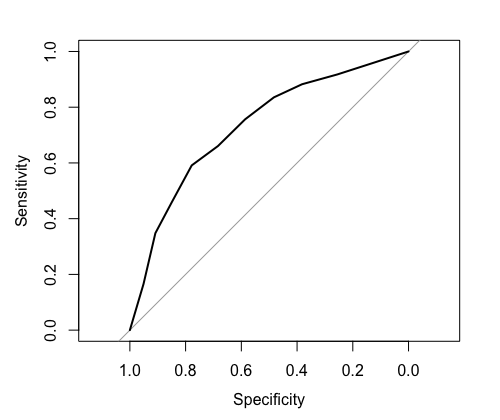
\includegraphics[width=0.5\linewidth]{/Users/tdounias/Desktop/Reed_Senior_Thesis/plots/roc_example} 
  
  }
  
  \caption[Example of an ROC curve]{Example of an ROC curve}\label{fig:roc example}
  \end{figure}
  
  Similarly to MSE, there is value in calculating AUC from a test dataset,
  rather than the dataset used to train the model. Therefore I also use
  5-fold cross-validation for AUC as well\footnote{This also compensates
    for models not converging, as some of mine do.}.
  
  \subsubsection{k-Folds Cross Validation}\label{k-folds-cross-validation}
  
  The goal of statistical modeling is to approximate the true function
  that links predictors to response. While the final model's coefficients
  should be estimated using as much data as possible, when assessing how
  good a fit that model is there can be better uses of the power that
  large amounts of data give us. k-Folds cross validation allows for
  better approximations of goodness-of-of-fit metrics, by partitioning the
  data into training datasets and test datasets. The fundamental idea is
  that the data is split into k different subsets, which are then
  sequentially used to fit the model and calculate the value of some
  metric(James et al., 2017). The algorithm goes as follows:
  
  \begin{enumerate}
  \item Partition data into k folds
  \item Fit model on all but the i-th fold
  \item Calculate goodness-of-fit metric on the i-th fold
  \item Repeat 2 and 3 for i$\in [0,k]$
  \item Calculate the average of all obtained goodness-of-fit measurements
  \end{enumerate}
  
  I perform 5-fold cross validation to calculate MSE and AUC for all
  models which I can fit in R.
  
  \chapter{Case Selection, Data, Model
  Parametrization}\label{case-selection-data-model-parametrization}
  
  \section{The Centennial State and Its
  Voters}\label{the-centennial-state-and-its-voters}
  
  \subsection{Demographics}\label{demographics}
  
  Colorado--named the Centennial State due to assuming statehood on the
  centennial of the Union--lies in the Southwestern United States, with
  its Western half squarely atop the Rocky Mountains. Based on its
  estimated population of just over 5.5 million, Colorado is the 21st most
  populous state, and ranks 37th in population density. The vast majority
  of that population is gathered in a series of urban areas that comprise
  a North-to-South strip in the middle of the state, containing the
  Denver-Aurora-Lakewood Metro Area, Colorado Springs, Pueblo, and Fort
  Collins. Apart from the Western town of Grand Junction, the rest of the
  population resides in vast rural areas.
  
  \begin{figure}
  
  {\centering 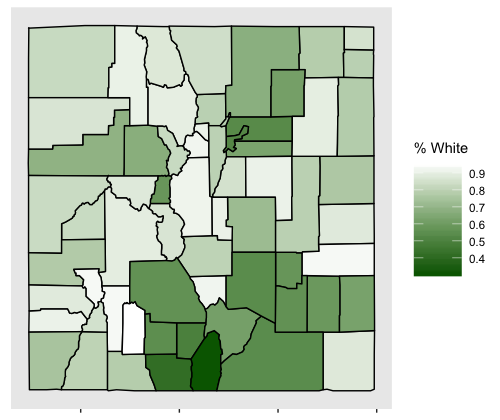
\includegraphics[width=0.8\linewidth]{/Users/tdounias/Desktop/Reed_Senior_Thesis/maps/pct_white_county_map} 
  
  }
  
  \caption[White voters per Colorado county]{White voters per Colorado county}\label{fig:white pct map}
  \end{figure}
  
  Colorado is landlocked, and far from any coastal town; in place of
  seaside resorts, Colorado attracts a substantial amount of tourists to
  its mountains every year. Therefore the more mountainous regions have
  developed skiing and mountaineering resorts. They also heavily depend on
  federal money and protection for national parks. These importance of
  these characteristics will become apparent in the following sections.
  
  Colorado has a median age of 34.3 and median household income of
  \$65,685. Colorado's population is mostly white, with a higher minority
  group population density in its Southern regions, as shown in figure
  3.1. (Bureau, 2010) The conclusion here is that Colorado is a relatively
  young, mostly white, and fairly well-off state that is increasingly
  getting more diverse, particularly in the South. These factors are
  important as they serve to associate Colorado with other states; such
  associations are useful for the replication of this study or the
  generalization of my results.
  
  The State Capital is Denver; Colorado is split into 64 Counties, of
  which the most populous are, in no particular order, the following: El
  Paso, Denver, Arapahoe, Jefferson, Adams, Larimer, Boulder, and Douglas.
  These counties comprise 73\% of the total population of Colorado.
  
  \begin{longtable}[]{@{}lccl@{}}
  \caption{Colorado population for largest counties
  \label{tab:pop_table}}\tabularnewline
  \toprule
  \begin{minipage}[b]{0.13\columnwidth}\raggedright\strut
  County\strut
  \end{minipage} & \begin{minipage}[b]{0.21\columnwidth}\centering\strut
  Total Population\strut
  \end{minipage} & \begin{minipage}[b]{0.20\columnwidth}\centering\strut
  CO Population \%\strut
  \end{minipage} & \begin{minipage}[b]{0.34\columnwidth}\raggedright\strut
  Largest Metro Area\strut
  \end{minipage}\tabularnewline
  \midrule
  \endfirsthead
  \toprule
  \begin{minipage}[b]{0.13\columnwidth}\raggedright\strut
  County\strut
  \end{minipage} & \begin{minipage}[b]{0.21\columnwidth}\centering\strut
  Total Population\strut
  \end{minipage} & \begin{minipage}[b]{0.20\columnwidth}\centering\strut
  CO Population \%\strut
  \end{minipage} & \begin{minipage}[b]{0.34\columnwidth}\raggedright\strut
  Largest Metro Area\strut
  \end{minipage}\tabularnewline
  \midrule
  \endhead
  \begin{minipage}[t]{0.13\columnwidth}\raggedright\strut
  Adams\strut
  \end{minipage} & \begin{minipage}[t]{0.21\columnwidth}\centering\strut
  441603\strut
  \end{minipage} & \begin{minipage}[t]{0.20\columnwidth}\centering\strut
  0.08781\strut
  \end{minipage} & \begin{minipage}[t]{0.34\columnwidth}\raggedright\strut
  Denver-Aurora-Lakewood\strut
  \end{minipage}\tabularnewline
  \begin{minipage}[t]{0.13\columnwidth}\raggedright\strut
  Arapahoe\strut
  \end{minipage} & \begin{minipage}[t]{0.21\columnwidth}\centering\strut
  572003\strut
  \end{minipage} & \begin{minipage}[t]{0.20\columnwidth}\centering\strut
  0.1137\strut
  \end{minipage} & \begin{minipage}[t]{0.34\columnwidth}\raggedright\strut
  Denver-Aurora-Lakewood\strut
  \end{minipage}\tabularnewline
  \begin{minipage}[t]{0.13\columnwidth}\raggedright\strut
  Boulder\strut
  \end{minipage} & \begin{minipage}[t]{0.21\columnwidth}\centering\strut
  294567\strut
  \end{minipage} & \begin{minipage}[t]{0.20\columnwidth}\centering\strut
  0.05857\strut
  \end{minipage} & \begin{minipage}[t]{0.34\columnwidth}\raggedright\strut
  Boulder\strut
  \end{minipage}\tabularnewline
  \begin{minipage}[t]{0.13\columnwidth}\raggedright\strut
  Denver\strut
  \end{minipage} & \begin{minipage}[t]{0.21\columnwidth}\centering\strut
  600158\strut
  \end{minipage} & \begin{minipage}[t]{0.20\columnwidth}\centering\strut
  0.1193\strut
  \end{minipage} & \begin{minipage}[t]{0.34\columnwidth}\raggedright\strut
  Denver\strut
  \end{minipage}\tabularnewline
  \begin{minipage}[t]{0.13\columnwidth}\raggedright\strut
  Douglas\strut
  \end{minipage} & \begin{minipage}[t]{0.21\columnwidth}\centering\strut
  285465\strut
  \end{minipage} & \begin{minipage}[t]{0.20\columnwidth}\centering\strut
  0.05676\strut
  \end{minipage} & \begin{minipage}[t]{0.34\columnwidth}\raggedright\strut
  Denver-Aurora-Lakewood\strut
  \end{minipage}\tabularnewline
  \begin{minipage}[t]{0.13\columnwidth}\raggedright\strut
  El Paso\strut
  \end{minipage} & \begin{minipage}[t]{0.21\columnwidth}\centering\strut
  622263\strut
  \end{minipage} & \begin{minipage}[t]{0.20\columnwidth}\centering\strut
  0.1237\strut
  \end{minipage} & \begin{minipage}[t]{0.34\columnwidth}\raggedright\strut
  Colorado Springs\strut
  \end{minipage}\tabularnewline
  \begin{minipage}[t]{0.13\columnwidth}\raggedright\strut
  Jefferson\strut
  \end{minipage} & \begin{minipage}[t]{0.21\columnwidth}\centering\strut
  534543\strut
  \end{minipage} & \begin{minipage}[t]{0.20\columnwidth}\centering\strut
  0.1063\strut
  \end{minipage} & \begin{minipage}[t]{0.34\columnwidth}\raggedright\strut
  Denver-Aurora-Lakewood\strut
  \end{minipage}\tabularnewline
  \begin{minipage}[t]{0.13\columnwidth}\raggedright\strut
  Larimer\strut
  \end{minipage} & \begin{minipage}[t]{0.21\columnwidth}\centering\strut
  299630\strut
  \end{minipage} & \begin{minipage}[t]{0.20\columnwidth}\centering\strut
  0.05958\strut
  \end{minipage} & \begin{minipage}[t]{0.34\columnwidth}\raggedright\strut
  Fort Collins\strut
  \end{minipage}\tabularnewline
  \begin{minipage}[t]{0.13\columnwidth}\raggedright\strut
  Other\strut
  \end{minipage} & \begin{minipage}[t]{0.21\columnwidth}\centering\strut
  1378964\strut
  \end{minipage} & \begin{minipage}[t]{0.20\columnwidth}\centering\strut
  0.2742\strut
  \end{minipage} & \begin{minipage}[t]{0.34\columnwidth}\raggedright\strut
  \strut
  \end{minipage}\tabularnewline
  \begin{minipage}[t]{0.13\columnwidth}\raggedright\strut
  Colorado\strut
  \end{minipage} & \begin{minipage}[t]{0.21\columnwidth}\centering\strut
  5029196\strut
  \end{minipage} & \begin{minipage}[t]{0.20\columnwidth}\centering\strut
  100\strut
  \end{minipage} & \begin{minipage}[t]{0.34\columnwidth}\raggedright\strut
  \strut
  \end{minipage}\tabularnewline
  \bottomrule
  \end{longtable}
  
  \clearpage
  
  \subsection{The Politics of Colorado}\label{the-politics-of-colorado}
  
  Curtis Martin (1962) notes that Colorado, due to its status as a
  frontier state, has always been fiercely democratic and independent. He
  connects this fact with Colorado's past, by pointing out that its
  political institutions were deeply rooted in mining culture, ordinary
  citizens' participation,a strong feeling of being ``far away'' from
  sources of centralized power in the coasts, and a wish for the
  protection and preservation of Colorado's natural environment. As such,
  Colorado can be described as a populist state with a strong libertarian
  streak, that highly values democratic processes when they serve the
  people or protect and fund national parks, but staunchly opposes state
  intervention when it is unwarranted. (Martin, 1962)
  
  This 1964 study of Colorado politics rings true to this day. One needs
  not search for long to see instances when Colorado honored this
  description. One example is TABOR, or the Taxpayer's Bill of Rights; a
  strongly libertarian, small-government, populist series of regulations
  that mandated a referendum for any measure that would increase state
  taxes, and caped government spending. TABOR was passed by referendum in
  1992, and later amended in 2005 after the dot com economic crisis
  exposed the fact that inability to spend is very bad for a state
  government trying to jump start its economy. (Assembly, n.d.)
  
  Similarly, Amendment 64 passed in 2012 made Colorado one of the first
  states to legalize the selling, possession, and consumption of
  recreational marijuana--a policy advocated by progressives and
  libertarians alike. Colorado was also the staging ground for what has
  been coined the ``Sagebrush Rebellion'': a movement primarily consisting
  on ranchers in dispute with the federal government over land use laws
  and wildlife protection. While this ``rebellion'' primarily consisted of
  battles in local legislatures or elections in the 1970s, its echoes can
  be heard till today in events like the Bundy Standoff, with ranchers
  taking up arms against federal employees and occupying federal land
  (Thompson, 2016).
  
  Setting policy aside, this description of Colorado is also confirmed by
  polling data and election results. While being traditionally more
  conservative, inflows of immigration from the South coupled with
  increasing urban liberalization and tourism has led the state from
  leaning republican to being aggressively purple: the quintessential
  swing state. Colorado voted both for and later against Bill Clinton,
  voted for G.W. Bush twice, and has supported democratic presidential
  candidates since (Hamm, 2017). The trend is also, maybe surprisingly,
  consistent when considering both rural and urban voters; the divide that
  is said to plague other states seems to have passed by Colorado.
  Additionally, when polled on trust of federal or local governments,
  Colorado residents are systematically skeptical; in a random sample poll
  conducted by Cronin and Loevy (2012) in 2010, 56\% stated that their
  state officials were lazy, wasteful, and inefficient. However--again
  indicating a libertarian, independent streak--most Coloradoans from 1988
  to today consistently believe that their state is ``on the right
  track.''\footnote{Colorado College Citizens Polls, taken from Cronin et
    al. (Cronin \& Loevy, 2012)}
  
  \subsection{Voting in Colorado}\label{voting-in-colorado}
  
  Each County individually administers local, coordinated, primary, and
  general elections, under the supervision of the Colorado Secretary of
  State. This means that each county individually handles the voters
  registered in that county. Unsurprisingly, the same eight most populous
  counties are also the counties with the majority of registered voters,
  as their registrants comprise 73\% of total Colorado registered voters
  (as of November 2017). As table 3.2 shows, these eight counties have a
  registration rate between 60-80\%, compared to a Colorado-wide rate of
  about 67\%. Registration rates for all counties are also graphically
  depicted in figure 3.2. In terms of Party registration, Colorado as a
  whole leans democratic by a very narrow margin (figure 3.3).
  
  \begin{longtable}[]{@{}lccc@{}}
  \caption{Colorado voter registration for largest counties
  \label{tab:voter_reg}}\tabularnewline
  \toprule
  \begin{minipage}[b]{0.10\columnwidth}\raggedright\strut
  County\strut
  \end{minipage} & \begin{minipage}[b]{0.24\columnwidth}\centering\strut
  Total Registered Voters\strut
  \end{minipage} & \begin{minipage}[b]{0.29\columnwidth}\centering\strut
  County Registration Rate\strut
  \end{minipage} & \begin{minipage}[b]{0.25\columnwidth}\centering\strut
  \% of Statewide Registrants\strut
  \end{minipage}\tabularnewline
  \midrule
  \endfirsthead
  \toprule
  \begin{minipage}[b]{0.10\columnwidth}\raggedright\strut
  County\strut
  \end{minipage} & \begin{minipage}[b]{0.24\columnwidth}\centering\strut
  Total Registered Voters\strut
  \end{minipage} & \begin{minipage}[b]{0.29\columnwidth}\centering\strut
  County Registration Rate\strut
  \end{minipage} & \begin{minipage}[b]{0.25\columnwidth}\centering\strut
  \% of Statewide Registrants\strut
  \end{minipage}\tabularnewline
  \midrule
  \endhead
  \begin{minipage}[t]{0.10\columnwidth}\raggedright\strut
  Adams\strut
  \end{minipage} & \begin{minipage}[t]{0.24\columnwidth}\centering\strut
  270,303\strut
  \end{minipage} & \begin{minipage}[t]{0.29\columnwidth}\centering\strut
  0.61\strut
  \end{minipage} & \begin{minipage}[t]{0.25\columnwidth}\centering\strut
  0.07\strut
  \end{minipage}\tabularnewline
  \begin{minipage}[t]{0.10\columnwidth}\raggedright\strut
  Arapahoe\strut
  \end{minipage} & \begin{minipage}[t]{0.24\columnwidth}\centering\strut
  410,546\strut
  \end{minipage} & \begin{minipage}[t]{0.29\columnwidth}\centering\strut
  0.72\strut
  \end{minipage} & \begin{minipage}[t]{0.25\columnwidth}\centering\strut
  0.11\strut
  \end{minipage}\tabularnewline
  \begin{minipage}[t]{0.10\columnwidth}\raggedright\strut
  Boulder\strut
  \end{minipage} & \begin{minipage}[t]{0.24\columnwidth}\centering\strut
  237,091\strut
  \end{minipage} & \begin{minipage}[t]{0.29\columnwidth}\centering\strut
  0.80\strut
  \end{minipage} & \begin{minipage}[t]{0.25\columnwidth}\centering\strut
  0.06\strut
  \end{minipage}\tabularnewline
  \begin{minipage}[t]{0.10\columnwidth}\raggedright\strut
  Denver\strut
  \end{minipage} & \begin{minipage}[t]{0.24\columnwidth}\centering\strut
  450,616\strut
  \end{minipage} & \begin{minipage}[t]{0.29\columnwidth}\centering\strut
  0.75\strut
  \end{minipage} & \begin{minipage}[t]{0.25\columnwidth}\centering\strut
  0.12\strut
  \end{minipage}\tabularnewline
  \begin{minipage}[t]{0.10\columnwidth}\raggedright\strut
  Douglas\strut
  \end{minipage} & \begin{minipage}[t]{0.24\columnwidth}\centering\strut
  237,659\strut
  \end{minipage} & \begin{minipage}[t]{0.29\columnwidth}\centering\strut
  0.83\strut
  \end{minipage} & \begin{minipage}[t]{0.25\columnwidth}\centering\strut
  0.06\strut
  \end{minipage}\tabularnewline
  \begin{minipage}[t]{0.10\columnwidth}\raggedright\strut
  El Paso\strut
  \end{minipage} & \begin{minipage}[t]{0.24\columnwidth}\centering\strut
  445,708\strut
  \end{minipage} & \begin{minipage}[t]{0.29\columnwidth}\centering\strut
  0.71\strut
  \end{minipage} & \begin{minipage}[t]{0.25\columnwidth}\centering\strut
  0.12\strut
  \end{minipage}\tabularnewline
  \begin{minipage}[t]{0.10\columnwidth}\raggedright\strut
  Jefferson\strut
  \end{minipage} & \begin{minipage}[t]{0.24\columnwidth}\centering\strut
  422,362\strut
  \end{minipage} & \begin{minipage}[t]{0.29\columnwidth}\centering\strut
  0.79\strut
  \end{minipage} & \begin{minipage}[t]{0.25\columnwidth}\centering\strut
  0.11\strut
  \end{minipage}\tabularnewline
  \begin{minipage}[t]{0.10\columnwidth}\raggedright\strut
  Larimer\strut
  \end{minipage} & \begin{minipage}[t]{0.24\columnwidth}\centering\strut
  250,626\strut
  \end{minipage} & \begin{minipage}[t]{0.29\columnwidth}\centering\strut
  0.84\strut
  \end{minipage} & \begin{minipage}[t]{0.25\columnwidth}\centering\strut
  0.06\strut
  \end{minipage}\tabularnewline
  \begin{minipage}[t]{0.10\columnwidth}\raggedright\strut
  Other\strut
  \end{minipage} & \begin{minipage}[t]{0.24\columnwidth}\centering\strut
  1,009,392\strut
  \end{minipage} & \begin{minipage}[t]{0.29\columnwidth}\centering\strut
  ---\strut
  \end{minipage} & \begin{minipage}[t]{0.25\columnwidth}\centering\strut
  0.27\strut
  \end{minipage}\tabularnewline
  \begin{minipage}[t]{0.10\columnwidth}\raggedright\strut
  Colorado\strut
  \end{minipage} & \begin{minipage}[t]{0.24\columnwidth}\centering\strut
  3,734,303\strut
  \end{minipage} & \begin{minipage}[t]{0.29\columnwidth}\centering\strut
  0.67\strut
  \end{minipage} & \begin{minipage}[t]{0.25\columnwidth}\centering\strut
  1.00\strut
  \end{minipage}\tabularnewline
  \bottomrule
  \end{longtable}
  
  \begin{figure}
  
  {\centering 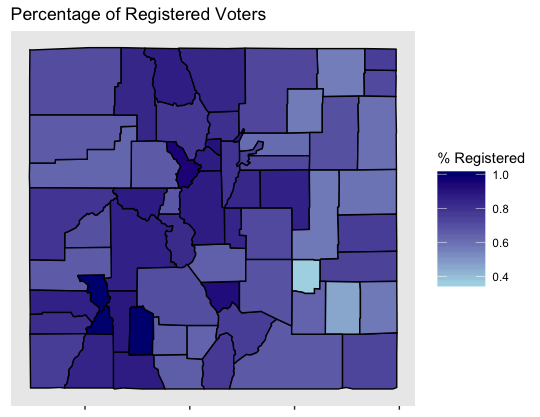
\includegraphics[width=0.8\linewidth]{/Users/tdounias/Desktop/Reed_Senior_Thesis/maps/pct_registered_county_map} 
  
  }
  
  \caption[Registration rates per Colorado county]{Registration rates per Colorado county}\label{fig:reg per county map}
  \end{figure}
  
  \begin{figure}
  
  {\centering 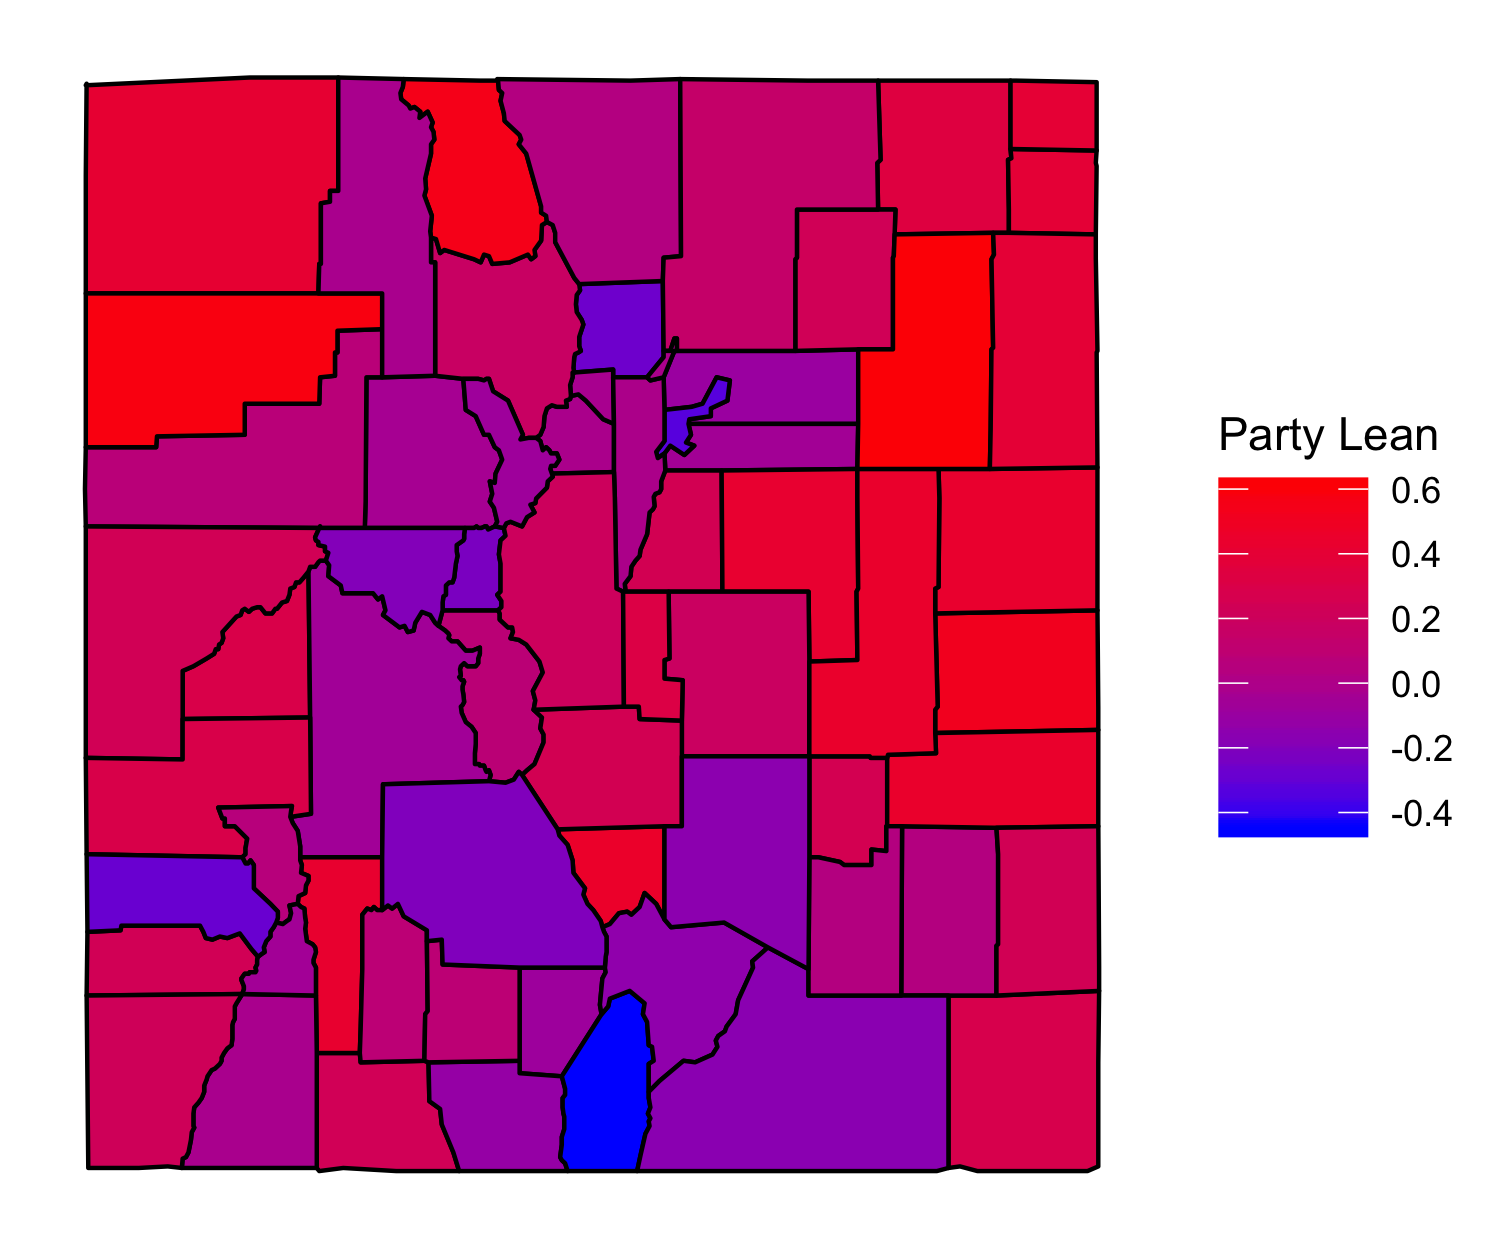
\includegraphics[width=0.8\linewidth]{/Users/tdounias/Desktop/Reed_Senior_Thesis/maps/party_affiliation_county_map} 
  
  }
  
  \caption[Democratic/Republican party lean per Colorado county]{Democratic/Republican party lean per Colorado county}\label{fig:party reg per county map}
  \end{figure}
  
  In the past 25 years, there have been a series of key changes in the way
  Colorado administers elections, in relation to Vote By Mail and other
  reforms targeted and expanding the democratic franchise. In 1992,
  Colorado introduced no-excuse absentee voting, allowing voters to either
  physically pick up a mail ballot at a Vote Center or County Office, or
  have a ballot mailed to them prior to election day. In 2008, this reform
  was expanded to a permanent Vote-By-Mail system, which gave counties the
  option to allow voters to be permanently put on a list of addresses that
  received mail ballots prior to the election. The State also entered a
  transitional status to full mail elections, giving counties the option
  to make all coordinated local elections, general elections, and primary
  elections exclusively VBM. In 2013, the Colorado State Legislature
  passed HB13-1303: The Voter Access and Modernized Elections Act, which
  mandated that every voter currently registered receive a mail ballot for
  all future elections. The Act also expanded the use of Vote Centers
  instead of traditional polling places, instituted same-day voter
  registration, and revamped the way active and inactive voter status was
  designated on voter rolls--more on this in future sections (Hullinghorst
  \& Pabon, 2013). These changes are summarized in Table 3.3.
  
  \begin{longtable}[]{@{}cl@{}}
  \caption{Key changes to Colorado elections policy
  \label{tab:elect_policy}}\tabularnewline
  \toprule
  \begin{minipage}[b]{0.07\columnwidth}\centering\strut
  Year\strut
  \end{minipage} & \begin{minipage}[b]{0.87\columnwidth}\raggedright\strut
  Key Changes\strut
  \end{minipage}\tabularnewline
  \midrule
  \endfirsthead
  \toprule
  \begin{minipage}[b]{0.07\columnwidth}\centering\strut
  Year\strut
  \end{minipage} & \begin{minipage}[b]{0.87\columnwidth}\raggedright\strut
  Key Changes\strut
  \end{minipage}\tabularnewline
  \midrule
  \endhead
  \begin{minipage}[t]{0.07\columnwidth}\centering\strut
  1992\strut
  \end{minipage} & \begin{minipage}[t]{0.87\columnwidth}\raggedright\strut
  No Excuse Absentee Statewide Implementation\strut
  \end{minipage}\tabularnewline
  \begin{minipage}[t]{0.07\columnwidth}\centering\strut
  2008\strut
  \end{minipage} & \begin{minipage}[t]{0.87\columnwidth}\raggedright\strut
  Permanent No-Excuse VBM Lists, Option of Full-VBM Elections\strut
  \end{minipage}\tabularnewline
  \begin{minipage}[t]{0.07\columnwidth}\centering\strut
  2013\strut
  \end{minipage} & \begin{minipage}[t]{0.87\columnwidth}\raggedright\strut
  Automatic Mail Ballot System Implemented Statewide, Established Vote
  Centers\strut
  \end{minipage}\tabularnewline
  \bottomrule
  \end{longtable}
  
  \clearpage
  
  \subsection{Colorado as a Case for this
  Thesis}\label{colorado-as-a-case-for-this-thesis}
  
  Colorado presents such an interesting case for research on Vote By Mail
  exactly because it has gone through such a long transitional process to
  reach its current elections system. It has steadily developed voting
  policy through a mixture of state mandates, county action, and outside
  policy motivations. Colorado's streak of independence and direct
  democracy is also very apparent in this shift in electoral practices,
  since they have been passing policies trying to expand participation for
  a very long time. It gives researchers access to approximately 22 years
  during which at least part of the state conducted elections partially by
  mail, making comparative, county- or individual- level case studies
  particularly alluring. Colorado's streak of independence and direct
  democracy is also very apparent in this shift in electoral practices,
  since they have been passing policies trying to expand participation for
  a very long time.
  
  On a more general level, Colorado is interesting exactly because it is
  ``typical'' but with a wild streak. It is typical rocky mountain
  country, great planes country, and liberal urban city but all \emph{in
  one state}. In is libertarian yet increasingly Democratic. It heavily
  relies on state funding for national parks, yet rebels against federal
  land use laws. It is a frontier state with traditional values, that
  overwhelmingly supports marijuana legalization. It is also a consistent
  purple state, with a Democratic Governor and House, but Republican
  Attorney General, Secretary of State and senate. This means that
  Colorado is a combination of distinct national effects, but also local
  effects that make it significantly different from national trends as a
  whole. In this environment, predicting results of policy can be
  difficult, but extremely salient as multiple effects can be tested
  against each other.
  
  \section{Acquiring the Data}\label{acquiring-the-data}
  
  This thesis relies on county and individual level models to draw
  conclusions on voting behaviors, and how they are affected by voting
  method. As such, the data I need will optimally contain the following:
  
  \begin{itemize}
  \item
    \textbf{County and individual level demographic characteristics}:
    race, gender, urban population
  \item
    \textbf{County and individual level voting data}: turnout, party
    registration, total registrants
  \item
    \textbf{Information on individual elections}: date, ballots cast,
    voting methods, county, election descriptions
  \end{itemize}
  
  In the process of my research, I have acquired sufficient data to cover
  the second and third of these areas. I was unable to procure individual
  level data on demographic characteristics apart from gender, age, and
  party registration. However, reasonable conclusions can still be drawn
  from county or precinct aggregates\footnote{}.
  
  \subsection{Sources and first glance}\label{sources-and-first-glance}
  
  I used two sources of data: Colorado voter records gathered by the
  Colorado Secretary of State's office, and demographic data from the 2010
  US Census. In the process of procuring these data I was aided by a
  series of other researchers and professionals with experience in the
  field of elections administration. Andrew Menger in particular was kind
  enough to give me access to data files for Colorado for the years of
  2012-2016 that he had already collected for his research\footnote{Doctor
    Menger's website with links to his research can be found at
    www.andrewmenger.com}. I directly obtained the 2017 from the Colorado
  Secretary of State's office, with the help of Mr.~Judd Choate, Director
  of Elections.
  
  \subsubsection{2010 US Census}\label{us-census}
  
  The US Census is conducted country-wide every ten years, with the goal
  of procuring accurate data on the demographic characteristics of the
  population. The Census uses a combination of federal field workers
  conducting door-to-door canvassing and statistical methods for data
  aggregation. From the 2010 Census--which is publicly available online--I
  get total population counts, characteristics on race, and rural/urban
  population counts for Colorado.
  
  I use two datasets from the Census. For both, the unit of observation is
  one of the 64 counties of Colorado, and both include the same total
  population counts. One contains racial demographic characteristics and
  the other contain percentages of rural and urban populations in each
  county. The racial demographic dataset needed some wrangling work to
  extract a percentage of white residents in each county. Individuals were
  coded as ``white'' when they identified as exclusively white--this
  doesn't include mixed-race individuals reporting white ancestry.
  
  \subsubsection{Colorado Voter Files}\label{colorado-voter-files}
  
  As any state, Colorado maintains a statewide registry of all currently
  registered voters. This registry is typically under the purview of the
  Secretary of State--in this case, Wayne W. Williams. Voter Registration
  Files are constantly updated with new information on existing voters,
  new voters, or with the removal of inactive or otherwise ineligible
  voters. Therefore, this file will be different every time it is accessed
  or shared. Based on when this file is accessed, only a ``snapshot'' of
  the file can be obtained. Similarly with VRFs, a Voter History File is
  maintained and constantly updated by the state. This file is uniquely
  connected to its VRF: only voters showing up as registrants will have
  their histories included. I have both Voter Registration and History
  files for the years between 2012-2017, obtained with the help of Judd
  Choate and Andrew Menger.
  
  In the Voter Registration files, the unit of observation is the
  individual voter, and all variables are initially coded as character
  strings. Each voter is assigned a unique voter ID, which serves as a
  point of reference between the two files. Broadly speaking, data in this
  file can be divided between three categories: first, personal
  identification information like address, ZIP code, or phone number;
  second, demographic information like age and gender; third, information
  pertinent to elections administration like congressional district, local
  elections for which the individual should receive a ballot, voter ID,
  and party registration. I will further elaborate on relevant variables
  in the wrangling section.
  
  In the Voter History files, the unit of observation here is a single
  ballot cast, and all variables are initially coded as character strings.
  This means that for each voter registered--and so included in the
  VRF--the history file should contain an observation for each time they
  voted. This file includes two types of data: first, identifiers for the
  election like county, date, description, and type; second, identifiers
  for the individual vote including voter ID and voting method.
  
  \section{Wrangling the Data}\label{wrangling-the-data}
  
  The process of ``wrangling'' refers to manipulating the data into a form
  that can then be used for graphing, exploratory data analysis,
  modelling, or presentation. In this case, wrangling also included
  aggregating data across multiple sources and datasets. For this purpose,
  I made heavy use of the tidyverse R package, and in particular the dplyr
  package. In this section I will go through some of the key problems
  encountered during the wrangling of these data, and then discuss the
  final form each variable takes.
  
  \subsection{Initial Problems with the 2017 Voter File and
  Solution}\label{initial-problems-with-the-2017-voter-file-and-solution}
  
  In my initial research, I intended to only use the 2017 snapshots of the
  Colorado Registration and History file. The major issue I
  encountered--which merits discussion in its own section, and
  necessitated that I search for more data--comes from the aforementioned
  fact that the records I had access to are ``snapshots''. What this
  means, is that for each person in each year of voter registration files,
  I have their corresponding history files for all ballots they have cast
  in Colorado, but not their own history of registration and migration.
  If, say, a voter moved from Boulder County to Summit County, I would
  have their votes in Boulder County show up in the voter history file,
  but them being registered in Summit. If you recall the turnout
  calculations specified earlier on, this implies an overestimation when
  looking back at elections that happened some time before the date of the
  ``snapshot''. Additionally, ``snapshots'' of current voter files do not
  reflect voters dropping off the rolls for whatever reason--death, moving
  out of the state, long term inactivity, non-confirmable personal data
  etc. Since for these voters the history files would also not be
  included, the issue created is less one of overestimation of turnout
  like before, but just the inclusion of additional room for error that is
  created when subtracting one from the denominator and enumerator of
  turnout.
  
  After going through turnout calculations with the 2017 files, a
  significant majority of counties appeared to have turnout exceeding
  80\%, particularly for years between 2000 and 2012. This was, to put it
  mildly, concerning. With the aforementioned help, I was given access to
  similar ``snapshots'' for each year between 2012-2016. After similar
  calculations, I returned figure 3.4 for the eight most populous counties
  as described above, including different shapes for election type, colors
  for county, and a vertical line at 2013 to signify the latest major
  change in how Colorado administers elections.
  
  \begin{figure}
  
  {\centering 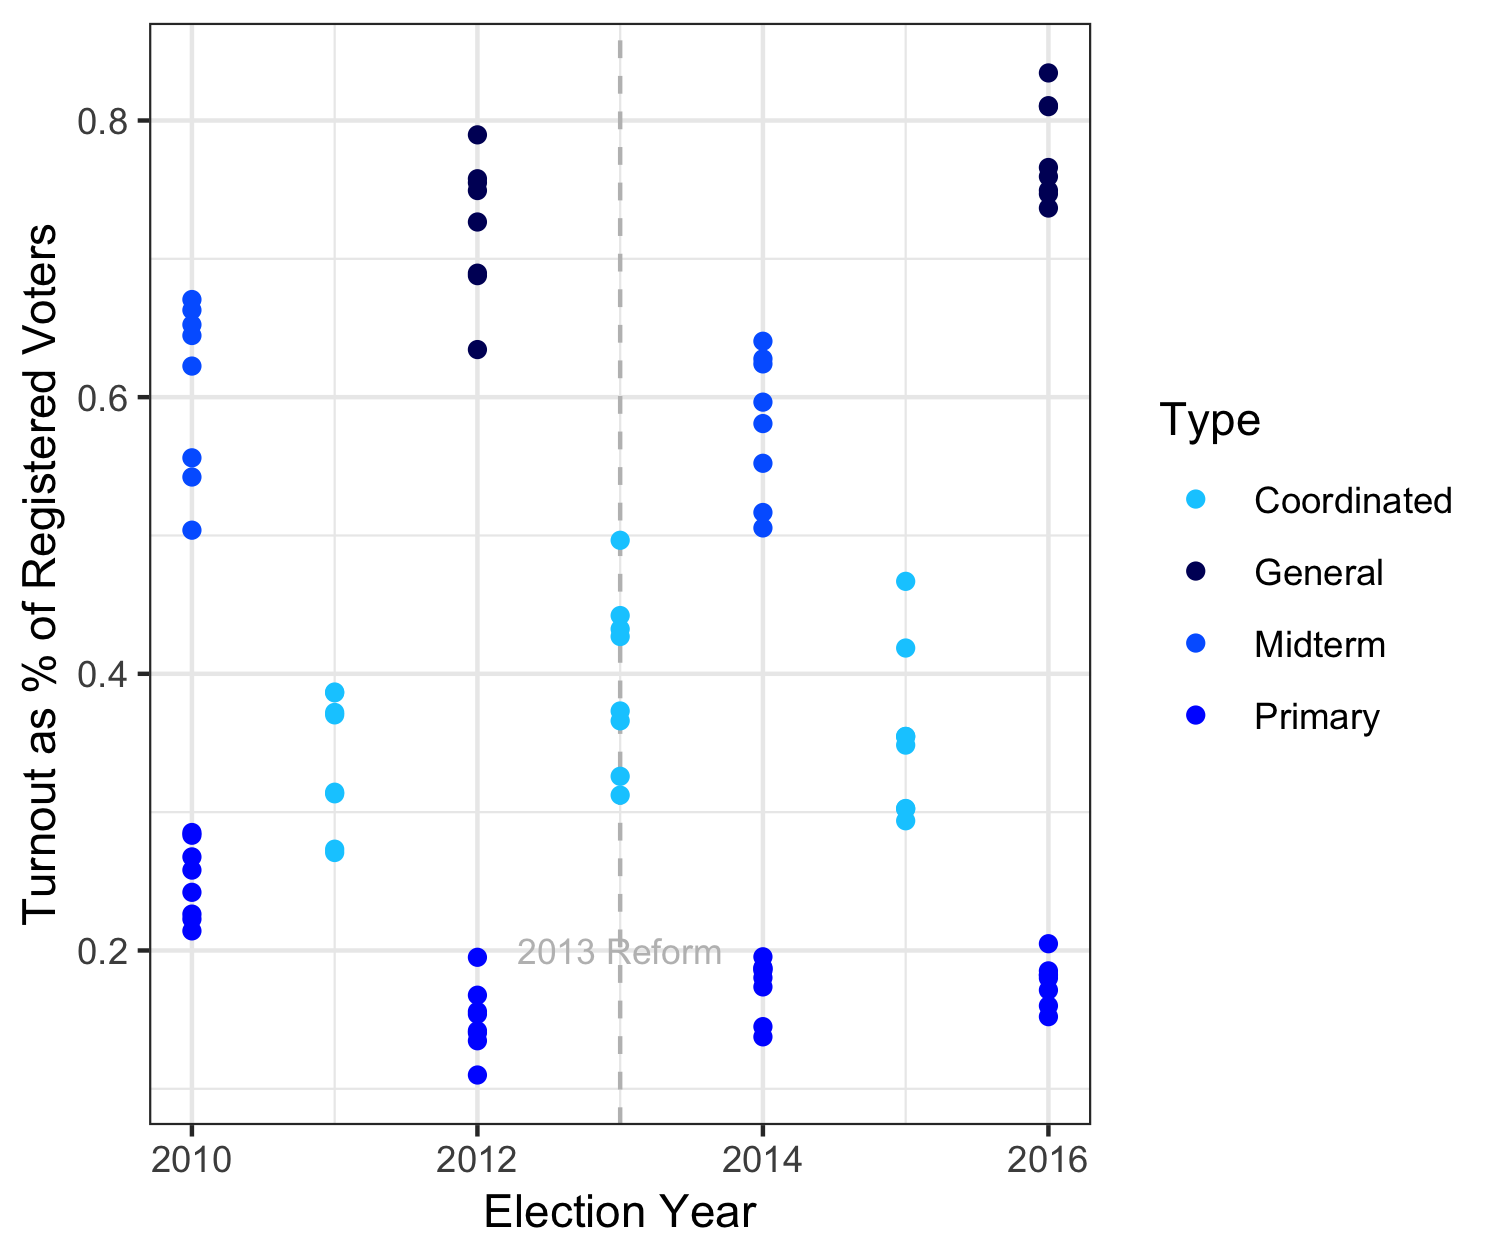
\includegraphics[width=0.8\linewidth]{/Users/tdounias/Desktop/Reed_Senior_Thesis/plots/colorado_bigeight_turnout_graph} 
  
  }
  
  \caption[Turnout plot for eight largest Colorado counties, 2012-2016]{Turnout plot for eight largest Colorado counties, 2012-2016}\label{fig:big eight turnout plot}
  \end{figure}
  
  To also further illustrate the in-county migration and dropped voter
  problem, I created a graph that includes logged total counts of
  registered voters calculated using the 2017 and the 2012-2016 files. The
  plot also includes a line at y=x. If in-Colorado migration and dropped
  voters are not an issue, most points on this graph should be at this
  line.
  
  \begin{figure}
  
  {\centering 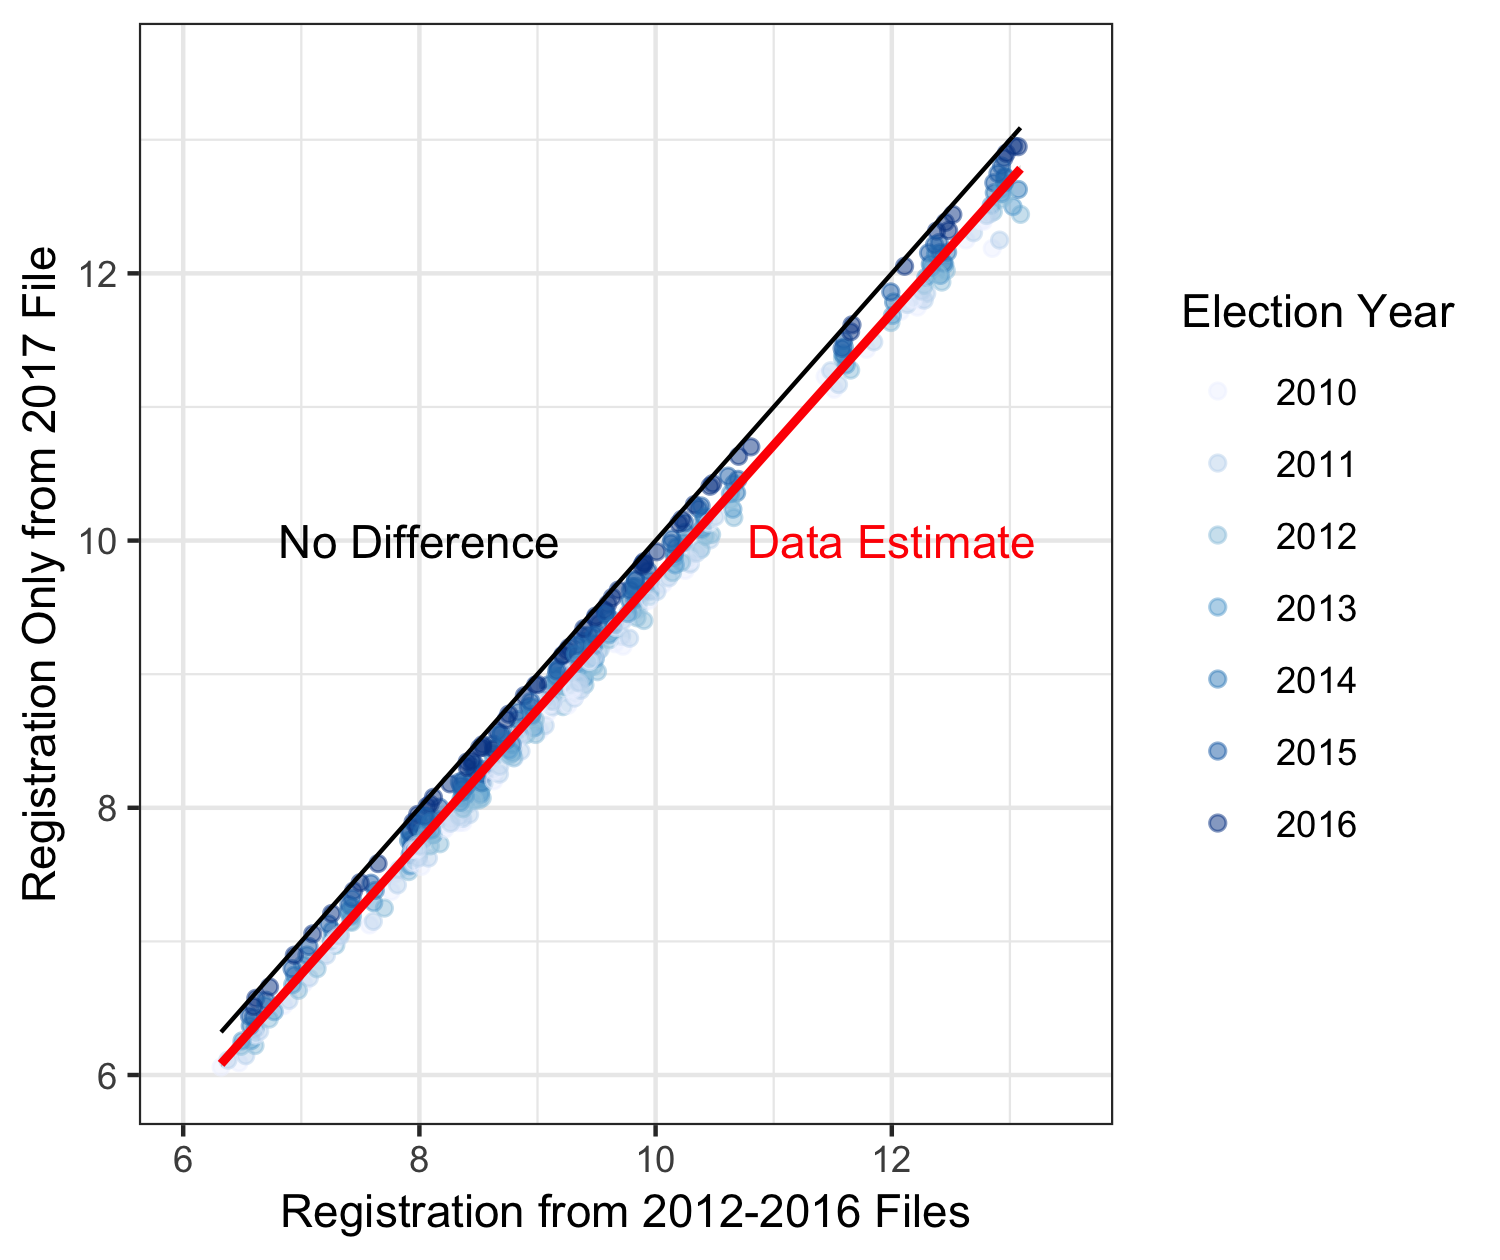
\includegraphics[width=0.8\linewidth]{/Users/tdounias/Desktop/Reed_Senior_Thesis/plots/county_migration_A} 
  
  }
  
  \caption[Comparison of registration count methods]{Comparison of registration count methods}\label{fig:county migration A}
  \end{figure}
  
  Two things should be clear from figure 3.5. First, there is significant
  deviation between the counts using just the 2017 file and all files
  across years. Specifically, the 2017 count consistently underestimates
  the total amount of registered voters--this is shown by the red linear
  model smoothing line. This consistent difference means that it is
  impossible to generate conclusions on my hypotheses using only the 2017
  files. Second, counts get more accurate the closer to 2017 we get. This
  should be even more apparent in figure 3.6, which limits the scale to
  only some high registration counties, and adds a shape indicator for
  county.
  
  \begin{figure}
  
  {\centering 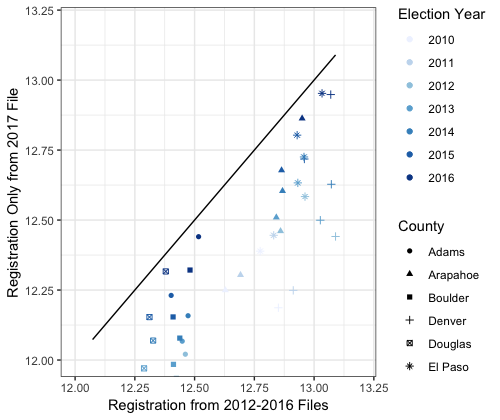
\includegraphics[width=0.8\linewidth]{/Users/tdounias/Desktop/Reed_Senior_Thesis/plots/county_migration_B} 
  
  }
  
  \caption[Comparison of registration count methods only for a few counties, 2012-2016]{Comparison of registration count methods only for a few counties, 2012-2016}\label{fig:county migration B}
  \end{figure}
  
  Here the structure of the data becomes clear: for each county, there are
  a series of almost vertically distributed points, which get closer to
  the y = x line the closer the counts get to 2017. Through this series of
  tests, it became clear that using multiple years of data was necessary
  in order to conduct an accurate test of my hypotheses. My selection was
  later vindicated, when looking at comparisons between reported rates of
  turnout\footnote{Turnout is calculated over all registered voters} and
  turnout calculated through my dataset for the 2014 midterm election (see
  fig. 3.7).
  
  \begin{figure}
  
  {\centering 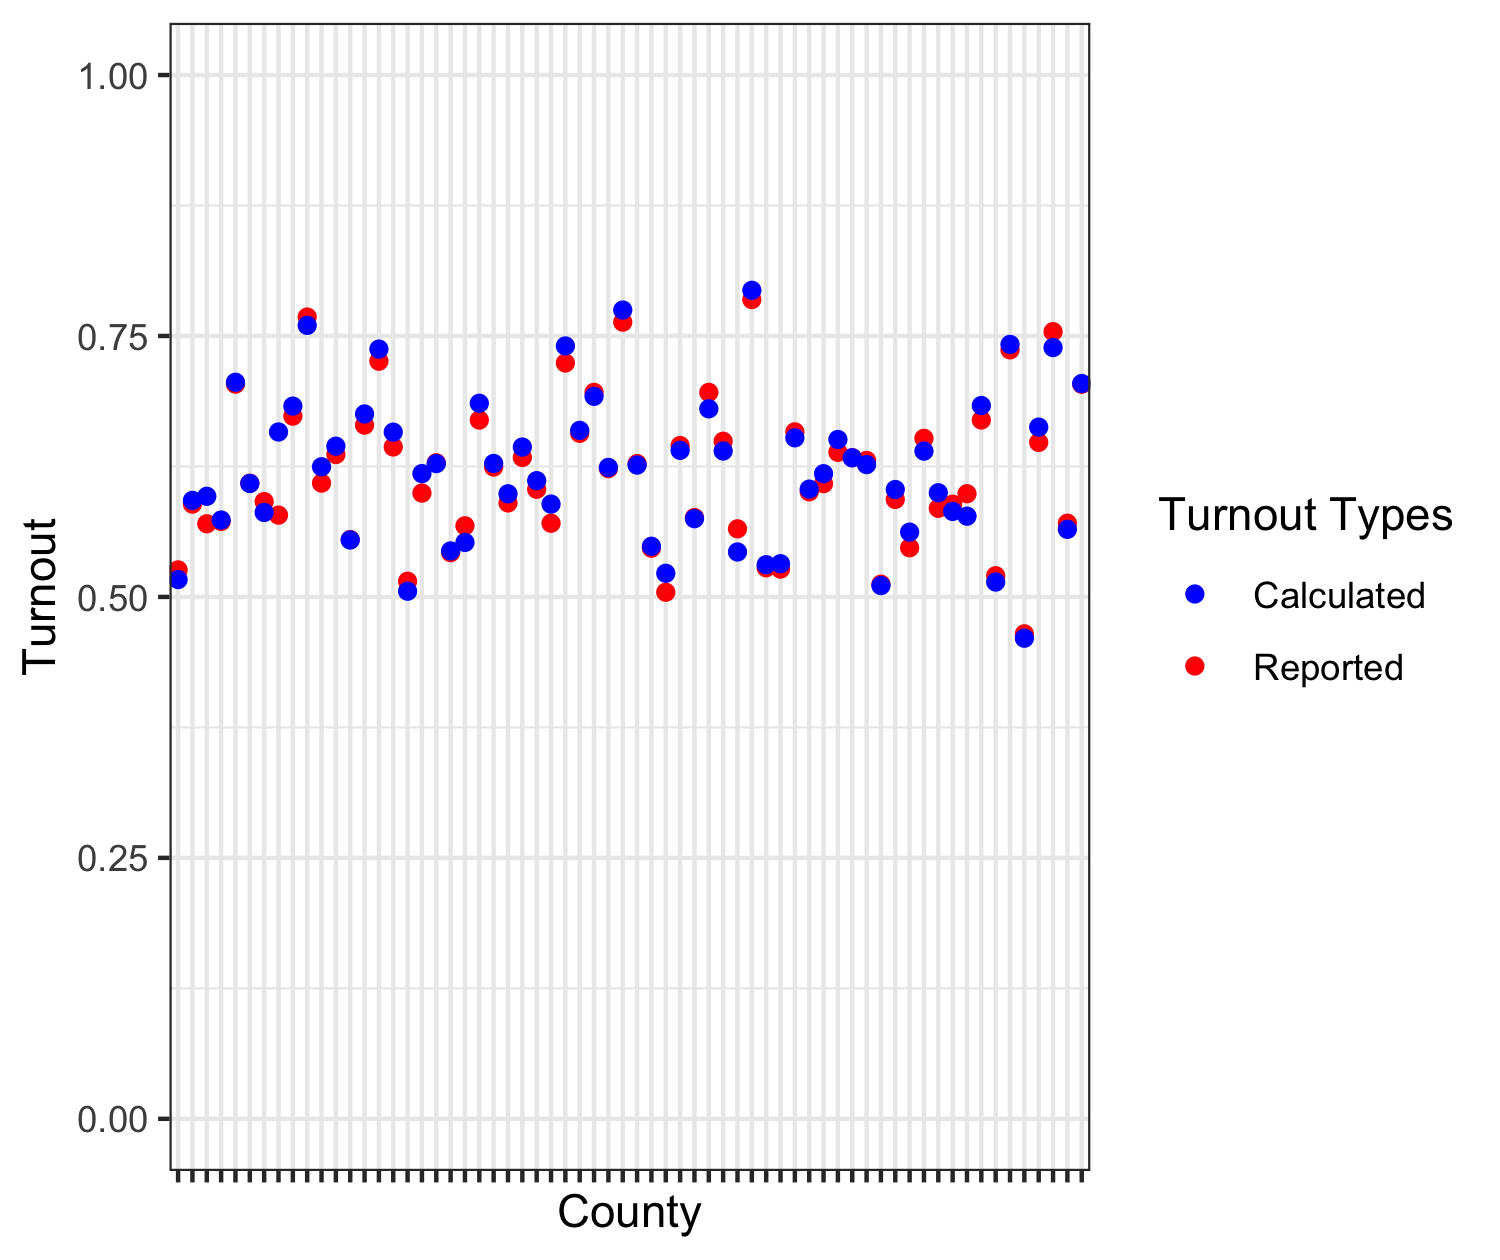
\includegraphics[width=0.8\linewidth]{/Users/tdounias/Desktop/Reed_Senior_Thesis/plots/Calc_vs_rep_turnout} 
  
  }
  
  \caption[Comparison of reported and calculated turnout for 2014 midterms across county]{Comparison of reported and calculated turnout for 2014 midterms across county}\label{fig:comp turnout 2014}
  \end{figure}
  
  The differences are insignificant. They exist because of ``noise'' added
  on because of errors in the data, misreporting, private voter
  registration files, voters dropped before the ``snapshot'' occurred, and
  other similar factors.
  
  \subsection{Other Wrangling Issues
  Faced}\label{other-wrangling-issues-faced}
  
  Wrangling the data was the majority of the work that went into this
  thesis. As will become clear in this section, apart from accurately
  processing, diagnosing, and merging the data, the process of wrangling
  includes several non-trivial decisions about how to treat missing values
  and variable specification. Doing a full account would probably read
  like the world's most cliche crime novel: a series of elusive final
  datasets, a plucky yet occasionally naive young detective, two wisened
  mentors, clues, dead ends, frustration, compromise,
  and\ldots{}spreadsheets. I will spare the reader the whole story, but I
  will include a non-comprehensive list of some of the difficulties
  associated with wrangling voter files, as it was a crucial part of the
  learning process I underwent while doing my research.
  
  \textbf{Missing Values}: The decision on how to deal with missing
  values--or NAs--in a dataset is a lot more important than it may
  initially seem. A first, intuitive reaction might be to just disregard
  them; however this works under the assumption that there is no structure
  inherent to why these data are missing! To give just two examples, in
  the data I have collected, the PARTY value for the 2015 voter
  registration file is missing. If I excluded all observations with
  missing PARTY values, I would be excluding a fifth of my data. Missing
  values were also present in the VOTING\_METHOD variable of the voter
  history files. While this may have seemed troubling, after closer
  examination it was revealed that the vast majority of such missing
  values was concentrated in Jefferson County, and in elections prior to
  2002. Therefore, these observations could be ignored, since they played
  no role in my final dataset. The conclusion should be that choices made
  on exclusion, inclusion, or estimation of missing data are very
  important, and should be taken with much care and consideration for the
  underlying structure of the data.
  
  \textbf{Data Input Errors}: Is ``QATAR'' a political party in Colorado?
  State records say not. However, ``QATAR'' did show up as a value in the
  Party variable for my 2016 voter registration file snapshot. This may
  occur for a number of reasons, the most likely of which is the
  introduction of errors when transferring these data. The data I have has
  been read and written by multiple operating systems (iOS and Windows)
  and programming platforms (STATA, R); they have also been uploaded,
  downloaded, and written unto CDs, as well as transferred between County
  and Colorado Secretary of State's Office when they were created.
  Characters that would be normally read into one platform as line or
  value delimiters may have been misinterpreted by another platform, with
  no operator error involved. In my analysis I treated all values that
  seemed more likely than not to be errors as NAs. There were not many of
  these--less than .001\% of my data--but they were a hassle to find,
  analyze, and then recode into some useful value.
  
  \textbf{Data Size}: Nothing to write home about here, just an
  observation that multiple voter registration files can be \emph{huge},
  which puts considerable strain on a computer's processing power. This
  means that wrangling has to comprise of a series of careful, deliberate
  moves. Brute force should be discouraged, as a dead end means several
  hours of melodic computer fan panic.
  
  \textbf{Joining, Merging, Spreading, and the Multiplicity of Levels}:
  For the data to end up in any functional shape, it eventually becomes
  necessary to start joining datasets. Thankfully, a clear division of
  modelling tasks between county and individual level models means that
  joining on COUNTY or VOTER\_ID is ideal, and fairly straightforward. As
  will become clear in later sections, I also had to consider the variety
  of different units of observation, specifically: county, individual,
  ballot, election, county-by-election.
  
  \subsection{Final Variable
  Specifications}\label{final-variable-specifications}
  
  After the conclusion of the wrangling process, the resulting dataset
  included a series of discrete and continuous variables. I will briefly
  outline them here, along with their range and values.
  
  \begin{itemize}
  \tightlist
  \item
    VOTER\_ID: Discrete variable, unique value given to each individual
    voter. Useful for merging.
  \item
    COUNTY: Discrete variable, the 64 counties of Colorado.
  \item
    REGISTRATION\_DATE: Discrete variable, date of registration for each
    registrant. Useful to get total registrants on election day.
  \item
    TURNOUT: Continuous variable, in the range {[}0,1{]}. The response
    variable for my county-level models.
  \item
    ELECTION\_TYPE: Discrete variable, the four types of elections:
    Primary, Coordinated, Midterm, Presidential.
  \item
    ELECTION\_DATE: Discrete variable, self-explanatory.
  \item
    VBM\_PCT: Continuous variable, in the range {[}0,1{]}. This is the
    focus of my analysis, as it counts the percentage of total ballots
    that were mail ballots.
  \item
    PCT\_WHITE: Continuous variable, in the range {[}0,1{]}. Percentage of
    white residents per county.
  \item
    PCT\_URBAN: Continuous variable, in the range {[}0,1{]}. Percentage of
    urban residents per county.
  \item
    PARTY: Discrete variable. For each voter, the party they are
    registered with. Can be: Republican, Democrat, Other, or Unaffiliated.
  \item
    GENDER: Discrete binary variable, Male or Female.
  \item
    AGE: The age of the individual registrant.
  \item
    VOTING\_METHOD: The method used by an individual voter to cast their
    ballot. Is coded as either VBM or In Person, according to Table 3.4:
  \end{itemize}
  
  \begin{longtable}[]{@{}lll@{}}
  \caption{Voting methods coding table
  \label{tab:voting_methods_table}}\tabularnewline
  \toprule
  \begin{minipage}[b]{0.22\columnwidth}\raggedright\strut
  Voting Method\strut
  \end{minipage} & \begin{minipage}[b]{0.42\columnwidth}\raggedright\strut
  Description of Method\strut
  \end{minipage} & \begin{minipage}[b]{0.18\columnwidth}\raggedright\strut
  Designation\strut
  \end{minipage}\tabularnewline
  \midrule
  \endfirsthead
  \toprule
  \begin{minipage}[b]{0.22\columnwidth}\raggedright\strut
  Voting Method\strut
  \end{minipage} & \begin{minipage}[b]{0.42\columnwidth}\raggedright\strut
  Description of Method\strut
  \end{minipage} & \begin{minipage}[b]{0.18\columnwidth}\raggedright\strut
  Designation\strut
  \end{minipage}\tabularnewline
  \midrule
  \endhead
  \begin{minipage}[t]{0.22\columnwidth}\raggedright\strut
  Absentee Carry\strut
  \end{minipage} & \begin{minipage}[t]{0.42\columnwidth}\raggedright\strut
  Voters who carried an absentee ballot with them from an early voting
  location or county office\strut
  \end{minipage} & \begin{minipage}[t]{0.18\columnwidth}\raggedright\strut
  VBM\strut
  \end{minipage}\tabularnewline
  \begin{minipage}[t]{0.22\columnwidth}\raggedright\strut
  Absentee Mail\strut
  \end{minipage} & \begin{minipage}[t]{0.42\columnwidth}\raggedright\strut
  Voters who were sent an absentee ballot, and mailed it in\strut
  \end{minipage} & \begin{minipage}[t]{0.18\columnwidth}\raggedright\strut
  VBM\strut
  \end{minipage}\tabularnewline
  \begin{minipage}[t]{0.22\columnwidth}\raggedright\strut
  Early Voting\strut
  \end{minipage} & \begin{minipage}[t]{0.42\columnwidth}\raggedright\strut
  Voters who physically went to an Early Voting location and voted\strut
  \end{minipage} & \begin{minipage}[t]{0.18\columnwidth}\raggedright\strut
  In Person\strut
  \end{minipage}\tabularnewline
  \begin{minipage}[t]{0.22\columnwidth}\raggedright\strut
  In Person\strut
  \end{minipage} & \begin{minipage}[t]{0.42\columnwidth}\raggedright\strut
  Voters who physically went to a polling place and voted on paper\strut
  \end{minipage} & \begin{minipage}[t]{0.18\columnwidth}\raggedright\strut
  In Person\strut
  \end{minipage}\tabularnewline
  \begin{minipage}[t]{0.22\columnwidth}\raggedright\strut
  Mail Ballot\strut
  \end{minipage} & \begin{minipage}[t]{0.42\columnwidth}\raggedright\strut
  Vote By Mail\strut
  \end{minipage} & \begin{minipage}[t]{0.18\columnwidth}\raggedright\strut
  VBM\strut
  \end{minipage}\tabularnewline
  \begin{minipage}[t]{0.22\columnwidth}\raggedright\strut
  Polling Place\strut
  \end{minipage} & \begin{minipage}[t]{0.42\columnwidth}\raggedright\strut
  Traditional polling place voting, discontinued in 2013\strut
  \end{minipage} & \begin{minipage}[t]{0.18\columnwidth}\raggedright\strut
  In Person\strut
  \end{minipage}\tabularnewline
  \begin{minipage}[t]{0.22\columnwidth}\raggedright\strut
  Vote Center\strut
  \end{minipage} & \begin{minipage}[t]{0.42\columnwidth}\raggedright\strut
  Voters who cast their ballots at Vote Centers\strut
  \end{minipage} & \begin{minipage}[t]{0.18\columnwidth}\raggedright\strut
  In Person\strut
  \end{minipage}\tabularnewline
  \bottomrule
  \end{longtable}
  
  \chapter{Model Specification and
  Results}\label{model-specification-and-results}
  
  \section{Modelling Issues}\label{modelling-issues}
  
  \subsection{Lack of variability}\label{lack-of-variability}
  
  To put it very simply, it's not enough to have hundreds of thousands of
  observations if they are all almost identical to each other. If, for
  example, my data included a thousand people in Jefferson county, and 63
  in all other counties of Colorado combined--one in each remaining
  county--, then I would not be able to leverage my data to draw
  conclusions on county-level effects.
  
  As previously stated, I have registration files going back to 2012. From
  these files, I have extracted data for elections going back to
  2010.\footnote{See section 3.3.1; I extracted data limited to this time
    period to avoid accuracy issues with migration and removal of
    inactive/unavailable voters} In order to make inferences on VBM and
  turnout effects I had to have extensive and varied data. I have
  extensive data--over 35 million observations at the individual
  level--but the data substantially lacks variance in voting method. Put
  simply, the vast majority of registrants in Colorado from 2010 onward
  either did not vote at all, or voted by mail. If you recall the changes
  in Colorado election law, in 2008 counties were allowed to conduct all
  mail elections, and no-excuse permanent absentee voting was implemented
  state-wide; then in 2013 Colorado transitioned to full VBM for all
  elections. This means that few people were still using traditional
  polling places or vote centers to cast their ballots. Figure 4.1 shows
  how, after 2013, and even before that in 2011--the coordinated, local
  election for which mail ballots were more convenient for counties--over
  95\% of ballots cast were mail ballots. Only in the general elections of
  2010 and 2012 there is some variance, but mail ballots account for well
  over two thirds of total votes.
  
  \begin{figure}
  
  {\centering 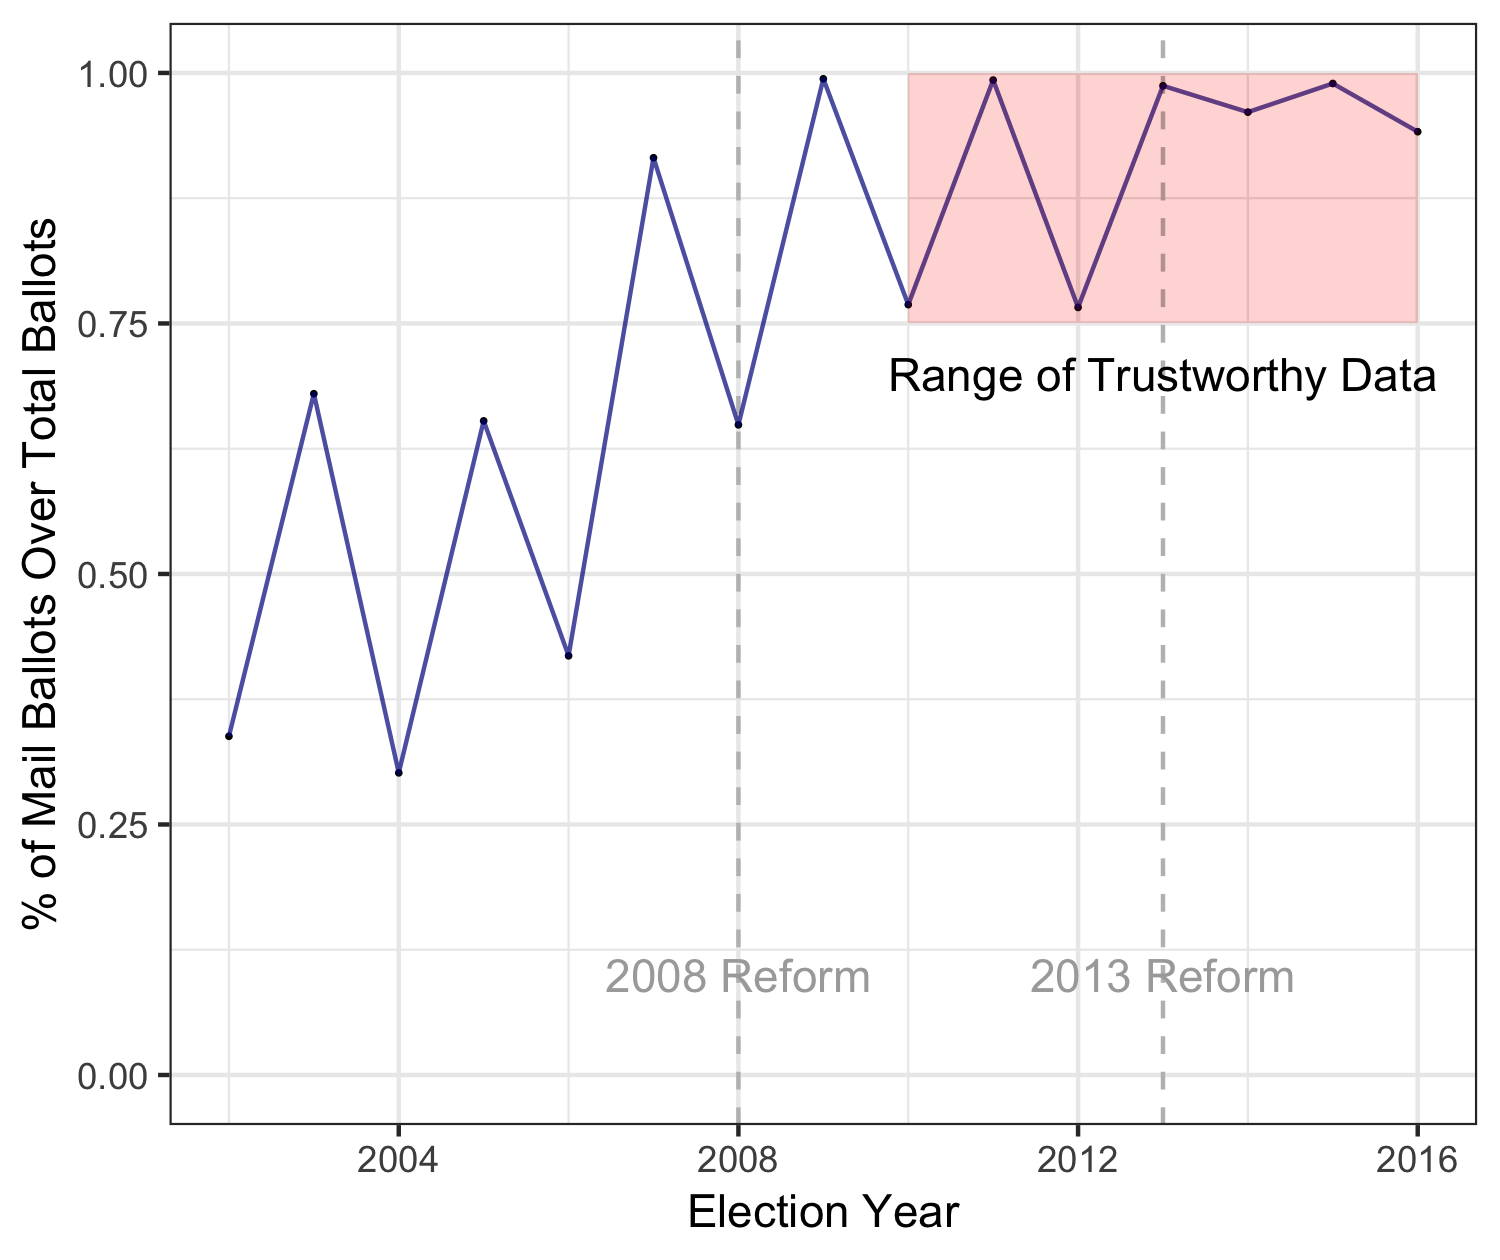
\includegraphics[width=0.8\linewidth]{/Users/tdounias/Desktop/Reed_Senior_Thesis/plots/vbm_county_graph} 
  
  }
  
  \caption[Percentage of mail ballots over total ballots by year]{Percentage of mail ballots over total ballots by year}\label{fig:vbm png}
  \end{figure}
  
  This issue is not completely fatal for my county level models. There is
  still variance between counties that have 100\% mail ballots and those
  that are around the 75-85\% margin. For individual level models--where I
  am estimating voting probability--VBM will be an almost perfect
  predictor for voting, and therefore will not present me with any
  substantial analytical result on how it affects voting probability.
  There are some ways to compensate for this issue, which I outline; due
  to time or data constraints, not all of these will be implemented in
  this thesis:
  
  \begin{itemize}
  \item
    \emph{More (Diverse) Data}: It would be very useful to get snapshot
    data of Colorado voter files from, say, 2004 to today, because it
    would allow for an extensive study on how the 2008 and 2013 election
    laws re-shaped voting decisions in the state. It would be amazing, but
    also expensive and very time consuming--involving several purchases of
    data from the Secretary of State of Colorado. Voter registration files
    also tend to get messier the further back one goes, which means that
    the process of cleaning up the data would get substantially harder. It
    would also require more processing power to handle more observations.
    My research here does not do this, as the scope of a senior thesis is
    a lot more limited than such an overarching study that would probably
    be conducted by multiple researchers with several assistants. I do
    however present several replicable materials for such a study, through
    the creation of an \textit{R} package I include on my gitHub page
    along with the final results of this thesis. This thesis does not go
    that far, but it may help similar studies in the future.
  \item
    \emph{Localized, Natural Experiment Studies}: A natural experiment is
    when, due to policy changes and circumstances, a ``control'' and
    ``treatment'' group of such a policy are created in the same
    approximate geographical area. This happens when, for example, only
    some of the counties in a state enact a specific change. Several such
    studies exist already, with some even tackling VBM in Colorado (Keele
    \& Titiunik, 2017), or how turnout rates are affected by new,
    restrictive registration laws (Burden \& Neiheisel, 2013). This method
    would allow for more accuracy in both the individual and county level
    models, and through the existence of a treatment and control group
    would guarantee the variability that I am currently lacking.
  \item
    \emph{Synthetic Control Group}: The synthetic control group method is
    a way of creating a control group when no such group seems to exist.
    It involves gathering a set of characteristics from the treatment
    group members and then using statistical methods to combine them into
    making the appropriate control (McClelland \& Gault, 2017). I will not
    go into the particulars of this method--the sources cited here should
    provide a decent introduction--, but this method has been successful
    in assessing policy effects such as anti-smoking laws (Barr et al.,
    2012), or even motor voter laws in Oregon(Gronke, McGhee, Romero, \&
    Griffin, 2017).
  \end{itemize}
  
  \subsection{Processing Power}\label{processing-power}
  
  The models are extremely RAM intensive; particularly the individual
  level models, for which I have almost 35 million different observations,
  do not run. For now, I compensated for this problem by using stratified
  sampling to sample a subset of my observations\footnote{A long term
    solution to this issue could be the use of a virtual machine, or some
    RStudio server, Or Amazon Work Spaces (AWS).}.
  
  The form of stratified sampling I am using is very simple; based on
  county, mail vote, and electoral participation, I use \texttt{dplyr} in
  \textit{R} to draw a sample that contains equal proportions of every
  combination of values of these variables to those in the original
  dataset. If, for example, the original dataset had 2\% of entries being
  voters from Jefferson county that participated using a mail ballot, the
  sampled dataset would have a proportion that is approximately equal to
  2\% (Chihara \& Hesterberg, 2011). In this way I draw a sample of around
  400,000 observations from my initial ballot dataset, on which I run all
  my individual models. After checking the variable ratios in sampled and
  population datasets, I found that the differences between ratios had a
  mean and standard deviation of less than a hundredth of a percentile.
  Therefore this sampled dataset could serve as a decent approximation of
  my population.
  
  \section{Variable Specification}\label{variable-specification}
  
  I will not go through each individual variable in this section, but will
  briefly describe my procedure on notation for the following models. I
  will include more comments whenever they seem necessary under each
  model. In this thesis I include predictors on a series of variables that
  can be divided into five categories based on unit of observation:
  county, election, individual, local result, and ballot. The last two are
  functions of other units: local result units are equal to the product of
  elections and counties, while ballot units are equal to the number of
  unique individuals multiplied by the number of elections each of them
  was registered in. For notation, I follow this set of rules:
  
  \begin{enumerate}
  \def\labelenumi{\arabic{enumi}.}
  \tightlist
  \item
    If the variable is a response, it is coded \(y\).
  \item
    If the variable is a predictor, it is coded according to Table 4.1.
  \item
    The variable's superscript will provide information on what it
    represents, else it will be explained.
  \item
    All variables represent a single value of that variable unless stated
    otherwise.
  \item
    Unit of observation will also be specified in subscript, according to
    the indices described in Table 4.1. These indices are also used in sum
    notation.
  \item
    All Greek characters represent coefficients to be calculated.
  \item
    By \(k[j]\) I represent the k-value of the j-observation. In this
    case, this would be the county that an individual is registered in.
  \item
    Note that for Local Result level variables, I use \(k,l\) as an
    indice. This is because there are very few variables at this level, it
    is a direct multiplicative product of two other units, and this
    notation avoids confusion with even more indice types.
  \end{enumerate}
  
  \begin{longtable}[]{@{}ccc@{}}
  \caption{Variable names and indices per unit of observation
  \label{tab:units_vars}}\tabularnewline
  \toprule
  \begin{minipage}[b]{0.27\columnwidth}\centering\strut
  Units\strut
  \end{minipage} & \begin{minipage}[b]{0.20\columnwidth}\centering\strut
  Variable\strut
  \end{minipage} & \begin{minipage}[b]{0.15\columnwidth}\centering\strut
  Index\strut
  \end{minipage}\tabularnewline
  \midrule
  \endfirsthead
  \toprule
  \begin{minipage}[b]{0.27\columnwidth}\centering\strut
  Units\strut
  \end{minipage} & \begin{minipage}[b]{0.20\columnwidth}\centering\strut
  Variable\strut
  \end{minipage} & \begin{minipage}[b]{0.15\columnwidth}\centering\strut
  Index\strut
  \end{minipage}\tabularnewline
  \midrule
  \endhead
  \begin{minipage}[t]{0.27\columnwidth}\centering\strut
  Ballot\strut
  \end{minipage} & \begin{minipage}[t]{0.20\columnwidth}\centering\strut
  u\strut
  \end{minipage} & \begin{minipage}[t]{0.15\columnwidth}\centering\strut
  i\strut
  \end{minipage}\tabularnewline
  \begin{minipage}[t]{0.27\columnwidth}\centering\strut
  Individual\strut
  \end{minipage} & \begin{minipage}[t]{0.20\columnwidth}\centering\strut
  z\strut
  \end{minipage} & \begin{minipage}[t]{0.15\columnwidth}\centering\strut
  j\strut
  \end{minipage}\tabularnewline
  \begin{minipage}[t]{0.27\columnwidth}\centering\strut
  County\strut
  \end{minipage} & \begin{minipage}[t]{0.20\columnwidth}\centering\strut
  x\strut
  \end{minipage} & \begin{minipage}[t]{0.15\columnwidth}\centering\strut
  k\strut
  \end{minipage}\tabularnewline
  \begin{minipage}[t]{0.27\columnwidth}\centering\strut
  Election\strut
  \end{minipage} & \begin{minipage}[t]{0.20\columnwidth}\centering\strut
  w\strut
  \end{minipage} & \begin{minipage}[t]{0.15\columnwidth}\centering\strut
  l\strut
  \end{minipage}\tabularnewline
  \begin{minipage}[t]{0.27\columnwidth}\centering\strut
  Local Result\strut
  \end{minipage} & \begin{minipage}[t]{0.20\columnwidth}\centering\strut
  v\strut
  \end{minipage} & \begin{minipage}[t]{0.15\columnwidth}\centering\strut
  k,l\strut
  \end{minipage}\tabularnewline
  \begin{minipage}[t]{0.27\columnwidth}\centering\strut
  General Index\strut
  \end{minipage} & \begin{minipage}[t]{0.20\columnwidth}\centering\strut
  -\strut
  \end{minipage} & \begin{minipage}[t]{0.15\columnwidth}\centering\strut
  i'\strut
  \end{minipage}\tabularnewline
  \bottomrule
  \end{longtable}
  
  \section{County Level Models}\label{county-level-models}
  
  \subsection{Specifications}\label{specifications}
  
  In this section I will go through a step-by step creation of models at
  the county level. County level models use a series of variables at the
  election, county, and local result levels. The response variable is
  always turnout as a local result. If this model is considered at its
  most basic, it could be thought of as an assignment of voting tendencies
  across counties; each county independent of election has a unique range
  of turnout results. In this way it is possible to build a naive,
  baseline model of turnout as follows:
  
  \begin{equation} \tag{Model 1}
  y^{turnout}_{k,l} = \beta_0 + (\sum_{k=1}^{64}\beta_kx_k^{county}),
  \end{equation}
  
  where \(x_k^{county}\) is a series of 64 dummy variables for each county
  of Colorado. Here differences between elections come from normally
  distributed error terms, rather than predictors. I name this
  \textbf{Model 1}, and it does not reflect the data particularly well.
  First off, this model includes the assumption that counties are
  independent of one another, which is probably false; just consider that
  these counties are areas of the same state, in the same country, with
  populations moving between them at regular intervals, and many of them
  covering the same metropolitan area or congressional district.
  Additionally, this model cannot fully calculate relevant coefficients,
  since a number of counties can be represented as perfect linear
  functions of the other variables. This means they will be dropped by
  \textit{R} when the model is called in the \texttt{lm()} function.
  
  A way to fix both these issues is to use a multilevel model with mixed
  effects for county. By constraining coefficients at the county level to
  a set distribution, this model does away with the assumption of
  independence. The other county level predictors help to explain some of
  the unexplained group level variation, which reduces the standard
  deviation of county coefficients and helps provide more exact estimates
  (Gelman \& Hill, 2006). I call this \textbf{Model 2}, which can be
  written as:
  
  \begin{equation} \tag{Model 2}
  y^{turnout}_{k,l} = a_{k} + \beta_{1}x_k^{\%white} + \beta_{2}x_k^{\%urban},
  \end{equation}
  
  \[a_{k} \sim N (\gamma_0, \sigma_{\alpha}^2)\] This model provides a
  more reasonable set of estimates for each county, but still fails at
  providing any information as to secular trends, time-specific effects,
  election type effects, or mail voting--the variable of interest. I will
  amend this by adding a set of variables at the election and local result
  levels: election type and an interaction term between election type and
  mail voting. This variable should reflect whether turnout effects of
  mail voting are more pronounced in a specific type of election. I call
  this \textbf{Model 3} and it can be specified as follows:
  
  \begin{equation} \tag{Model 3}
  y^{turnout}_{k,l} = a_{k} + \beta_{1}x_k^{\% white} + \beta_{2}x_k^{\% urban} + (\sum_{i'=1}^{4}\beta_{i'+3}w_{i'}^{election type})*(\beta_3v_{k,l}^{\% mail~vote} + 1),
  \end{equation}
  
  \[a_{k} \sim N(\gamma_0, \sigma_{\alpha}^2)\]
  
  where \(w_{i'}^{election type}\) is a series of four dummy variables for
  each type of election (General, Primary, Coordinated, Midterm). This
  model reflects nearly all the information I have available, apart from
  election date. For the incorporation of election dates there are two
  possible alternatives. First, I can simply add a dummy variable for each
  year. This would assume independence between each year, as it would
  specify different, independent ``slopes'' for the seven years I have
  data for--this is like calculating seven different models, one for each
  year. This is not particularly elegant as a solution nor does it reflect
  the fact that years actually are interconnected; of course there can be
  massive shifts in national or regional political climates, but those
  shifts happened \emph{from some baseline}, which is reflected in
  previous years.
  
  These elections can be thought of as systems for which prior condition
  affects future outcomes, and therefore time cannot be modeled as a
  series of independent effects. The solution here is adding a spline
  function for time, using a general additive multilevel model. The most
  commonly used spline function, and the default in the \texttt{gamm4}
  \textit{R} package is a thin plate regression spline, which I also use
  here (S. N. Wood, 2006). More on the subject of splines can be found in
  the Wood (2006) textbook. The model, which I call \textbf{Model 4} can
  be written as follows:
  
  \begin{equation}\tag{Model 4}
  y^{turnout}_{k,l} = a_{k} + \beta_{1}x_k^{\% white} + \beta_{2}x_k^{\% urban} + (\sum_{i'=1}^{4}\beta_{i'+3}w_{i'}^{election type})*(\beta_3v_{k,l}^{\% mail vote} + 1) + s(w^{year}_{l}),
  \end{equation}
  
  \[a_{k} \sim N(\gamma_0, \sigma_{\alpha}^2)\] where \(s()\) is a natural
  cubic regression spline function with seven knots--equal to the number
  of years.\footnote{I used the \texttt{gam.check()} function that is
    present in the \texttt{mgcv} \textit{R} package, whose call determined
    that the number of knots here may be too low. However, given the data
    available to me, I was limited to the inclusion of seven years and as
    such cannot increase the number of knots any further. Setting the
    number of knots to seven also gave the lowest CV MSE.} A summary of
  these four models is provided in the following table:
  
  \begin{longtable}[]{@{}ll@{}}
  \caption{County level model descriptions
  \label{tab:model_desc_county}}\tabularnewline
  \toprule
  \begin{minipage}[b]{0.15\columnwidth}\raggedright\strut
  Model No\strut
  \end{minipage} & \begin{minipage}[b]{0.80\columnwidth}\raggedright\strut
  Model Description\strut
  \end{minipage}\tabularnewline
  \midrule
  \endfirsthead
  \toprule
  \begin{minipage}[b]{0.15\columnwidth}\raggedright\strut
  Model No\strut
  \end{minipage} & \begin{minipage}[b]{0.80\columnwidth}\raggedright\strut
  Model Description\strut
  \end{minipage}\tabularnewline
  \midrule
  \endhead
  \begin{minipage}[t]{0.15\columnwidth}\raggedright\strut
  Model 1\strut
  \end{minipage} & \begin{minipage}[t]{0.80\columnwidth}\raggedright\strut
  Naive model with only county specific effects\strut
  \end{minipage}\tabularnewline
  \begin{minipage}[t]{0.15\columnwidth}\raggedright\strut
  Model 2\strut
  \end{minipage} & \begin{minipage}[t]{0.80\columnwidth}\raggedright\strut
  Multilevel model; added county level predictors\strut
  \end{minipage}\tabularnewline
  \begin{minipage}[t]{0.15\columnwidth}\raggedright\strut
  Model 3\strut
  \end{minipage} & \begin{minipage}[t]{0.80\columnwidth}\raggedright\strut
  Multilevel model; added VBM, interaction terms, and election fixed
  effects\strut
  \end{minipage}\tabularnewline
  \begin{minipage}[t]{0.15\columnwidth}\raggedright\strut
  Model 4\strut
  \end{minipage} & \begin{minipage}[t]{0.80\columnwidth}\raggedright\strut
  Multilevel General Additive model; added spline function for election
  year\strut
  \end{minipage}\tabularnewline
  \bottomrule
  \end{longtable}
  
  \subsection{Results}\label{results}
  
  The table in this section presents coefficients and standard errors for
  all four county level models. This table does not include any metrics
  for county--either mixed or fixed effects. I have chosen to omit these
  because they firstly are not very relevant to my hypotheses, and
  secondly because they are very extensive--64 coefficients for each of
  the four models. I have also not included any metric for time--here
  measured in years and used only in the fourth model. Both the mixed
  effects for county and the measure for time should be considered as
  controls: the first controls for county-specific trends while still
  restricting these to allow for non-independence, and the second makes
  sure that my results are indicative of a secular trend, accounting for
  any shifts along time.
  
  In terms of goodness-of-fit, I use 5-fold cross-validated Mean Squared
  Error (MSE) for all of the models. There is a significant drop-off in
  MSE between models 1,2 and models 3.4 of around \(.35\), which shows
  that the variables introduced in the later models substantially increase
  how well the models explain variability in the data. There is also a
  small increase of CV MSE between models 3 and 4, but the numbers are
  very comparable\footnote{If I was trying to make a model for predictive
    purposes I would probably choose Model 3; however, there is still
    value in comparing models 3 and 4, even if the later doesn't fit the
    data better than 3. The difference in coefficient values, after
    controlling for time, is a particularly interesting result.}.
  
  \begin{longtable}[]{@{}lcccc@{}}
  \caption{Estimated county level coefficients
  \label{tab:county_coef}}\tabularnewline
  \toprule
  \begin{minipage}[b]{0.26\columnwidth}\raggedright\strut
  Variables\strut
  \end{minipage} & \begin{minipage}[b]{0.12\columnwidth}\centering\strut
  Model 1\strut
  \end{minipage} & \begin{minipage}[b]{0.14\columnwidth}\centering\strut
  Model 2\strut
  \end{minipage} & \begin{minipage}[b]{0.14\columnwidth}\centering\strut
  Model 3\strut
  \end{minipage} & \begin{minipage}[b]{0.11\columnwidth}\centering\strut
  Model 4\strut
  \end{minipage}\tabularnewline
  \midrule
  \endfirsthead
  \toprule
  \begin{minipage}[b]{0.26\columnwidth}\raggedright\strut
  Variables\strut
  \end{minipage} & \begin{minipage}[b]{0.12\columnwidth}\centering\strut
  Model 1\strut
  \end{minipage} & \begin{minipage}[b]{0.14\columnwidth}\centering\strut
  Model 2\strut
  \end{minipage} & \begin{minipage}[b]{0.14\columnwidth}\centering\strut
  Model 3\strut
  \end{minipage} & \begin{minipage}[b]{0.11\columnwidth}\centering\strut
  Model 4\strut
  \end{minipage}\tabularnewline
  \midrule
  \endhead
  \begin{minipage}[t]{0.26\columnwidth}\raggedright\strut
  (Intercept)\strut
  \end{minipage} & \begin{minipage}[t]{0.12\columnwidth}\centering\strut
  0.369\strut
  \end{minipage} & \begin{minipage}[t]{0.14\columnwidth}\centering\strut
  0.492\strut
  \end{minipage} & \begin{minipage}[t]{0.14\columnwidth}\centering\strut
  0.455\strut
  \end{minipage} & \begin{minipage}[t]{0.11\columnwidth}\centering\strut
  0.470\strut
  \end{minipage}\tabularnewline
  \begin{minipage}[t]{0.26\columnwidth}\raggedright\strut
  \strut
  \end{minipage} & \begin{minipage}[t]{0.12\columnwidth}\centering\strut
  (0.60)\strut
  \end{minipage} & \begin{minipage}[t]{0.14\columnwidth}\centering\strut
  (0.045)**\strut
  \end{minipage} & \begin{minipage}[t]{0.14\columnwidth}\centering\strut
  (0.078)**\strut
  \end{minipage} & \begin{minipage}[t]{0.11\columnwidth}\centering\strut
  (0.072)\strut
  \end{minipage}\tabularnewline
  \begin{minipage}[t]{0.26\columnwidth}\raggedright\strut
  Pct\_white\strut
  \end{minipage} & \begin{minipage}[t]{0.12\columnwidth}\centering\strut
  \strut
  \end{minipage} & \begin{minipage}[t]{0.14\columnwidth}\centering\strut
  0.034\strut
  \end{minipage} & \begin{minipage}[t]{0.14\columnwidth}\centering\strut
  0.033\strut
  \end{minipage} & \begin{minipage}[t]{0.11\columnwidth}\centering\strut
  0.031\strut
  \end{minipage}\tabularnewline
  \begin{minipage}[t]{0.26\columnwidth}\raggedright\strut
  \strut
  \end{minipage} & \begin{minipage}[t]{0.12\columnwidth}\centering\strut
  \strut
  \end{minipage} & \begin{minipage}[t]{0.14\columnwidth}\centering\strut
  (0.053)\strut
  \end{minipage} & \begin{minipage}[t]{0.14\columnwidth}\centering\strut
  (0.050)\strut
  \end{minipage} & \begin{minipage}[t]{0.11\columnwidth}\centering\strut
  (0.050)\strut
  \end{minipage}\tabularnewline
  \begin{minipage}[t]{0.26\columnwidth}\raggedright\strut
  Pct\_urban\strut
  \end{minipage} & \begin{minipage}[t]{0.12\columnwidth}\centering\strut
  \strut
  \end{minipage} & \begin{minipage}[t]{0.14\columnwidth}\centering\strut
  -0.118\strut
  \end{minipage} & \begin{minipage}[t]{0.14\columnwidth}\centering\strut
  -0.117\strut
  \end{minipage} & \begin{minipage}[t]{0.11\columnwidth}\centering\strut
  -0.119\strut
  \end{minipage}\tabularnewline
  \begin{minipage}[t]{0.26\columnwidth}\raggedright\strut
  \strut
  \end{minipage} & \begin{minipage}[t]{0.12\columnwidth}\centering\strut
  \strut
  \end{minipage} & \begin{minipage}[t]{0.14\columnwidth}\centering\strut
  (0.022)**\strut
  \end{minipage} & \begin{minipage}[t]{0.14\columnwidth}\centering\strut
  (0.021)**\strut
  \end{minipage} & \begin{minipage}[t]{0.11\columnwidth}\centering\strut
  (0.021)\strut
  \end{minipage}\tabularnewline
  \begin{minipage}[t]{0.26\columnwidth}\raggedright\strut
  typeGeneral\strut
  \end{minipage} & \begin{minipage}[t]{0.12\columnwidth}\centering\strut
  \strut
  \end{minipage} & \begin{minipage}[t]{0.14\columnwidth}\centering\strut
  \strut
  \end{minipage} & \begin{minipage}[t]{0.14\columnwidth}\centering\strut
  0.190\strut
  \end{minipage} & \begin{minipage}[t]{0.11\columnwidth}\centering\strut
  0.254\strut
  \end{minipage}\tabularnewline
  \begin{minipage}[t]{0.26\columnwidth}\raggedright\strut
  \strut
  \end{minipage} & \begin{minipage}[t]{0.12\columnwidth}\centering\strut
  \strut
  \end{minipage} & \begin{minipage}[t]{0.14\columnwidth}\centering\strut
  \strut
  \end{minipage} & \begin{minipage}[t]{0.14\columnwidth}\centering\strut
  (0.070)**\strut
  \end{minipage} & \begin{minipage}[t]{0.11\columnwidth}\centering\strut
  (0.065)\strut
  \end{minipage}\tabularnewline
  \begin{minipage}[t]{0.26\columnwidth}\raggedright\strut
  typeMidterm\strut
  \end{minipage} & \begin{minipage}[t]{0.12\columnwidth}\centering\strut
  \strut
  \end{minipage} & \begin{minipage}[t]{0.14\columnwidth}\centering\strut
  \strut
  \end{minipage} & \begin{minipage}[t]{0.14\columnwidth}\centering\strut
  0.252\strut
  \end{minipage} & \begin{minipage}[t]{0.11\columnwidth}\centering\strut
  0.070\strut
  \end{minipage}\tabularnewline
  \begin{minipage}[t]{0.26\columnwidth}\raggedright\strut
  \strut
  \end{minipage} & \begin{minipage}[t]{0.12\columnwidth}\centering\strut
  \strut
  \end{minipage} & \begin{minipage}[t]{0.14\columnwidth}\centering\strut
  \strut
  \end{minipage} & \begin{minipage}[t]{0.14\columnwidth}\centering\strut
  (0.068)**\strut
  \end{minipage} & \begin{minipage}[t]{0.11\columnwidth}\centering\strut
  (0.063)\strut
  \end{minipage}\tabularnewline
  \begin{minipage}[t]{0.26\columnwidth}\raggedright\strut
  typePrimary\strut
  \end{minipage} & \begin{minipage}[t]{0.12\columnwidth}\centering\strut
  \strut
  \end{minipage} & \begin{minipage}[t]{0.14\columnwidth}\centering\strut
  \strut
  \end{minipage} & \begin{minipage}[t]{0.14\columnwidth}\centering\strut
  -0.071\strut
  \end{minipage} & \begin{minipage}[t]{0.11\columnwidth}\centering\strut
  -0.170\strut
  \end{minipage}\tabularnewline
  \begin{minipage}[t]{0.26\columnwidth}\raggedright\strut
  \strut
  \end{minipage} & \begin{minipage}[t]{0.12\columnwidth}\centering\strut
  \strut
  \end{minipage} & \begin{minipage}[t]{0.14\columnwidth}\centering\strut
  \strut
  \end{minipage} & \begin{minipage}[t]{0.14\columnwidth}\centering\strut
  (0.069)\strut
  \end{minipage} & \begin{minipage}[t]{0.11\columnwidth}\centering\strut
  (0.062)\strut
  \end{minipage}\tabularnewline
  \begin{minipage}[t]{0.26\columnwidth}\raggedright\strut
  typeCoordinated*VBM\strut
  \end{minipage} & \begin{minipage}[t]{0.12\columnwidth}\centering\strut
  \strut
  \end{minipage} & \begin{minipage}[t]{0.14\columnwidth}\centering\strut
  \strut
  \end{minipage} & \begin{minipage}[t]{0.14\columnwidth}\centering\strut
  -0.001\strut
  \end{minipage} & \begin{minipage}[t]{0.11\columnwidth}\centering\strut
  0.002\strut
  \end{minipage}\tabularnewline
  \begin{minipage}[t]{0.26\columnwidth}\raggedright\strut
  \strut
  \end{minipage} & \begin{minipage}[t]{0.12\columnwidth}\centering\strut
  \strut
  \end{minipage} & \begin{minipage}[t]{0.14\columnwidth}\centering\strut
  \strut
  \end{minipage} & \begin{minipage}[t]{0.14\columnwidth}\centering\strut
  (0.067)\strut
  \end{minipage} & \begin{minipage}[t]{0.11\columnwidth}\centering\strut
  (0.058)\strut
  \end{minipage}\tabularnewline
  \begin{minipage}[t]{0.26\columnwidth}\raggedright\strut
  typeGeneral*VBM\strut
  \end{minipage} & \begin{minipage}[t]{0.12\columnwidth}\centering\strut
  \strut
  \end{minipage} & \begin{minipage}[t]{0.14\columnwidth}\centering\strut
  \strut
  \end{minipage} & \begin{minipage}[t]{0.14\columnwidth}\centering\strut
  0.151\strut
  \end{minipage} & \begin{minipage}[t]{0.11\columnwidth}\centering\strut
  0.087\strut
  \end{minipage}\tabularnewline
  \begin{minipage}[t]{0.26\columnwidth}\raggedright\strut
  \strut
  \end{minipage} & \begin{minipage}[t]{0.12\columnwidth}\centering\strut
  \strut
  \end{minipage} & \begin{minipage}[t]{0.14\columnwidth}\centering\strut
  \strut
  \end{minipage} & \begin{minipage}[t]{0.14\columnwidth}\centering\strut
  (0.073)*\strut
  \end{minipage} & \begin{minipage}[t]{0.11\columnwidth}\centering\strut
  (0.037)\strut
  \end{minipage}\tabularnewline
  \begin{minipage}[t]{0.26\columnwidth}\raggedright\strut
  typeMidterm*VBM\strut
  \end{minipage} & \begin{minipage}[t]{0.12\columnwidth}\centering\strut
  \strut
  \end{minipage} & \begin{minipage}[t]{0.14\columnwidth}\centering\strut
  \strut
  \end{minipage} & \begin{minipage}[t]{0.14\columnwidth}\centering\strut
  -0.058\strut
  \end{minipage} & \begin{minipage}[t]{0.11\columnwidth}\centering\strut
  0.109\strut
  \end{minipage}\tabularnewline
  \begin{minipage}[t]{0.26\columnwidth}\raggedright\strut
  \strut
  \end{minipage} & \begin{minipage}[t]{0.12\columnwidth}\centering\strut
  \strut
  \end{minipage} & \begin{minipage}[t]{0.14\columnwidth}\centering\strut
  \strut
  \end{minipage} & \begin{minipage}[t]{0.14\columnwidth}\centering\strut
  (0.026)\strut
  \end{minipage} & \begin{minipage}[t]{0.11\columnwidth}\centering\strut
  (0.030)\strut
  \end{minipage}\tabularnewline
  \begin{minipage}[t]{0.26\columnwidth}\raggedright\strut
  typePrimary*VBM\strut
  \end{minipage} & \begin{minipage}[t]{0.12\columnwidth}\centering\strut
  \strut
  \end{minipage} & \begin{minipage}[t]{0.14\columnwidth}\centering\strut
  \strut
  \end{minipage} & \begin{minipage}[t]{0.14\columnwidth}\centering\strut
  -0.089\strut
  \end{minipage} & \begin{minipage}[t]{0.11\columnwidth}\centering\strut
  -0.003\strut
  \end{minipage}\tabularnewline
  \begin{minipage}[t]{0.26\columnwidth}\raggedright\strut
  \strut
  \end{minipage} & \begin{minipage}[t]{0.12\columnwidth}\centering\strut
  \strut
  \end{minipage} & \begin{minipage}[t]{0.14\columnwidth}\centering\strut
  \strut
  \end{minipage} & \begin{minipage}[t]{0.14\columnwidth}\centering\strut
  (0.028)\strut
  \end{minipage} & \begin{minipage}[t]{0.11\columnwidth}\centering\strut
  (0.027)\strut
  \end{minipage}\tabularnewline
  \begin{minipage}[t]{0.26\columnwidth}\raggedright\strut
  CV MSE\strut
  \end{minipage} & \begin{minipage}[t]{0.12\columnwidth}\centering\strut
  0.041\strut
  \end{minipage} & \begin{minipage}[t]{0.14\columnwidth}\centering\strut
  0.040\strut
  \end{minipage} & \begin{minipage}[t]{0.14\columnwidth}\centering\strut
  0.004\strut
  \end{minipage} & \begin{minipage}[t]{0.11\columnwidth}\centering\strut
  0.006\strut
  \end{minipage}\tabularnewline
  \begin{minipage}[t]{0.26\columnwidth}\raggedright\strut
  Obs\strut
  \end{minipage} & \begin{minipage}[t]{0.12\columnwidth}\centering\strut
  704\strut
  \end{minipage} & \begin{minipage}[t]{0.14\columnwidth}\centering\strut
  704\strut
  \end{minipage} & \begin{minipage}[t]{0.14\columnwidth}\centering\strut
  704\strut
  \end{minipage} & \begin{minipage}[t]{0.11\columnwidth}\centering\strut
  704\strut
  \end{minipage}\tabularnewline
  \begin{minipage}[t]{0.26\columnwidth}\raggedright\strut
  Groups\strut
  \end{minipage} & \begin{minipage}[t]{0.12\columnwidth}\centering\strut
  64\strut
  \end{minipage} & \begin{minipage}[t]{0.14\columnwidth}\centering\strut
  64\strut
  \end{minipage} & \begin{minipage}[t]{0.14\columnwidth}\centering\strut
  64\strut
  \end{minipage} & \begin{minipage}[t]{0.11\columnwidth}\centering\strut
  64\strut
  \end{minipage}\tabularnewline
  \bottomrule
  \end{longtable}
  
  Given that, the first observable result is that the percentage of white
  population and the percentage of urban population are fairly stable
  indicators of a small positive and negative shift in turnout
  respectively, although only urban population reaches statistical
  significance at the .05 level. The lack of variability between models is
  not surprising; these represent a county-level, time-independent
  demographic statistic, and there would be no reason to assume that part
  of their effect would be subsumed by other variables in models 3 and 4.
  
  Moving on to election type, the first thing to note is that there is no
  typeCoordinated in the table. This is because of the way \textit{R}
  displays and calculates models for discrete variables, when they are
  coded as indicators. The coefficients for the different election types
  should be read as differences from the ``baseline'' that is
  typeCoordinated. First surprising result here is that the coefficient
  for general presidential elections is substantially lower than that of
  midterms. Rather, this would be surprising if we did not notice the
  interaction terms with VBM, which indicate that after allowing for VBM
  effects, presidential elections do actually have higher turnout in my
  model than midterms do\footnote{Remember here that due to Figure 4.1
    most counties will have a proportion of mail ballots close to .9}.
  Other than this, coefficients in model 3 and model 4 make sense, in the
  assumed ordering of turnout in such elections: presidential, then
  midterm, then coordinated and primary.
  
  Next, taking election type and all interaction terms into consideration,
  let's examine what happens when the spline function for time is
  introduced between models 3 and 4. Most coefficients shift dramatically,
  with the exception of the interaction between coordinated elections and
  VBM. This dramatic shift--between 5 and 15(!) percentage
  points--indicates that several of the effects that the third model
  estimated are actually time-specific trends, and that there is a
  significant difference if we account for them. In the fourth model, the
  coefficients for election type on their own are still indicative of a
  common assumption for turnout in such elections\footnote{Also see Figure
    3.4}. As for interaction terms with VBM, the effect of VBM on primary
  election turnout is almost wiped out entirely, the interaction with
  general election turnout is depleted but still present at around 8\%,
  and coordinated election VBM effects remain statistically insignificant.
  Interestingly, the effect of VBM on midterm turnout switches sign from a
  negative effect of 5\% to a positive effect of around 11\%.
  
  Taking my hypotheses one by one, these models present evidence less in
  favor of H1, than against its alternate, H1'. While mail voting does
  seem to affect turnout in a way consistent across time--see the
  coefficients for VBM effects on general and midterm elections--this
  effect is not particularly more strong than the percentage of urban
  population in each county. Conversely, my second and third hypotheses
  can be convincingly rejected at the county level. After controlling for
  time, the effect that VBM has on coordinated or primary elections is not
  statistically significant, compared to significant, consistent effects
  on midterm and general elections. The one point in favor of H3 here is
  that the effect of VBM on midterm elections is slightly higher--about
  2\%--than the effect on presidential elections in model 4. However, this
  difference is not enough to rule in favor of H3; if this difference was
  caused by the lack of presence of national effects, it would be more
  pronounced in primary and coordinated elections.
  
  \section{Individual Level Models}\label{individual-level-models}
  
  \subsection{Specifications}\label{specifications-1}
  
  For the rest of this section, assume the following:
  
  \[y_i \sim \text{Bernoulli}(p)\]
  
  Where \(y_i \in \{0,1\}\) is the probability that the i-th ballot was
  completed.
  
  If receiving a ballot with no information, I would predict that the
  probability that an additional ballot was a vote in favor would be equal
  to turnout, as calculated through all other ballots. Therefore:
  
  \[\hat{\mathbb{P}}(y_i = 1) = \frac{\# \text{votes cast}}{\# \text{ballots}}\]
  
  \subsubsection{Estimation with only one type of
  data}\label{estimation-with-only-one-type-of-data}
  
  There are four levels of data I will go through here: County, Election,
  Person, and Ballot.
  
  \subsubsection{County Level}\label{county-level}
  
  Assume that the ballot I am trying to assess completion for has the name
  of the county it is from written on it. There are two ways to predict
  \(\mathbb{P(y_i = 1)}\). First, assume that each different county has a
  different, independent \(\mathbb{P(y_i = 1)}\), then:
  
  \[\hat{\mathbb{P}}(y_i = 1) \sim \text{logit}^{-1}(\sum_{k = 1}^{64}x_{k,i}\beta_{k})\]
  
  Where k counts over the 64 counties of Colorado, and \(x_{k}\) is an
  indicator variable for each county. If I, quite reasonably, throw away
  the assumption of independence--these counties are, after all, in the
  same state and the same country--I could also fit a mixed effects model
  as such:
  
  \begin{equation} \tag{Model 1}
  \hat{\mathbb{P}}(y_i = 1) \sim \text{logit}^{-1}(a_{k[i]}),
  \end{equation}
  
  \[a_{k} \sim \text{N}(\gamma_0, \sigma_{\alpha}^2)\]
  
  Where \(\alpha_{k[i]}\) varies by county, constrained by its standard
  deviation and \(\gamma_0\), an intercept coefficient. I name this
  \textbf{Model 1}.
  
  Let's say now that along with the one ballot, I was given a short list
  of \(n^{\text{county vars}}\) other county-level variables, be they
  discrete, continuous, or indicators. The two models would then look
  like:
  
  \[\hat{\mathbb{P}}(y_i = 1) \sim \text{logit}^{-1}(\sum_{k = 1}^{64}x_{k}\beta_{k} + \sum_{i'=1}^{n^{\text{county vars}}}x_{k[i], i'}\beta_{i'+64})\]
  
  Where \(x_{k[i], l}\) is the k-th value of the i'-th variable. If, as
  before, I do not assume independence, the model can be written as:
  
  \begin{equation} \tag{Model 2}  
  \hat{\mathbb{P}}(y_i = 1) \sim \text{logit}^{-1}(a_{k[i]}),
  \end{equation}
  
  \[a_{k} \sim \text{N}(\gamma_0 + \sum_{i'=1}^{n^{\text{county vars}}}x_{k[i], i'}\gamma_{i'}, \sigma_{\alpha}^2)\]
  
  In the case of my specific data, for the time being I have county-level
  data for white population and urban population, so
  \(n^{\text{county vars}} = 2\). I name this \textbf{Model 2}
  
  \subsubsection{Individual Level}\label{individual-level}
  
  Assuming that I know the voter ID of the individual that cast their
  ballot, I can treat this piece of information in about the same way that
  I did for county as described above. This means that the following is
  mostly an exercise in maintaining notation constant. For these purposes,
  let \(n^{ID}\) be the number of total unique voter
  IDs--individuals--that I have data on, and j an indice that sums over
  all individuals. Also let \(z_{j}\) be an indicator variable for each
  individual. Then:
  
  \[\hat{\mathbb{P}}(y_i = 1) \sim \text{logit}^{-1}(\sum_{j = 1}^{n^{ID}}z_{j}\beta_{j})\]
  
  And the second model, not assuming independence, would be:
  
  \[\hat{\mathbb{P}}(y_i = 1) \sim \text{logit}^{-1}(\delta_{j[i]}), \]
  \[\delta_{j} \sim \text{N}(\zeta_0, \sigma_{\delta}^2)\]
  
  Again, in a similar way to county level data, there are variables at an
  individual level, thus making it relatively easy to build further
  models. Let's say now that along with the one ballot, I was given a
  short list of \(n^{\text{indiv vars}}\) other individual-level
  variables, be they discrete, continuous, or indicators. The two models
  would then look like:
  
  \[\hat{\mathbb{P}}(y_i = 1) \sim \text{logit}^{-1}(\sum_{j = 1}^{n^{ID}}z_{j}\beta_{j} + \sum_{i'=1}^{n^{\text{indiv vars}}}z_{j[i], i'}\beta_{i'+n^{ID}})\]
  
  Where \(z_{j[i], l}\) is the j-th value of the i'-th variable. If, as
  before, I do not assume independence, the model can be written as:
  
  \begin{equation} \tag{Model 3*}
  \hat{\mathbb{P}}(y_i = 1) \sim \text{logit}^{-1}(\delta_{j[i]}),
  \end{equation}
  
  \[\delta_{j} \sim \text{N}(\zeta_0 + \sum_{i'=1}^{n^{\text{indiv vars}}}z_{j[i], i'}\delta_{i'}, \sigma_{\delta}^2)\]
  
  In the case of my specific data, for the time being I have
  individual-level data for gender, so \(n^{\text{indiv vars}} = 1\). I
  name the combination of this model and Model 2: \textbf{Model 3}.
  
  \subsubsection{Election Level}\label{election-level}
  
  Again as previously, four models come from including election level
  data. The first two are assuming I only knew what specific election the
  ballot comes from. Let \(w_{i'}\) be an indicator variable for each
  election and \(n^{elect}\) the number of elections. The model assuming
  independence, with \(w_{i'}\) being indicator variables for each
  election, is:
  
  \[\hat{\mathbb{P}}(y_i = 1) \sim \text{logit}^{-1}(\sum_{l = 1}^{n^{elect}}w_{l}\beta_{l})\]
  
  Again, as previously, it would be safe to assume that each election is
  not held in a vacuum. Adding mixed effects this model would be:
  
  \[\hat{\mathbb{P}}(y_i = 1) \sim \text{logit}^{-1}(\eta_{l[i]}), \]
  \[\eta_{l} \sim \text{N}(\nu_0, \sigma_{\nu}^2)\]
  
  Again, in a similar way to county and individual level data, I add in
  variables at an election level. Let's say now that along with the one
  ballot, I was given a short list of \(n^{\text{election vars}}\) other
  election-level variables, be they discrete, continuous, or indicators.
  The two models would then look like:
  
  \begin{equation} \tag{Model 4}
  \hat{\mathbb{P}}(y_i = 1) \sim \text{logit}^{-1}(\sum_{l = 1}^{n^{elect}}w_{l}\beta_{l} + \sum_{i'=1}^{n^{\text{election vars}}}w_{l[i], i'}\beta_{i'+n^{elect}})
  \end{equation}
  
  Where \(w_{l[i], i'}\) is the l-th value of the i'-th variable. For the
  time being I have two different variables that describe individual
  elections: date and type. I choose to fit a glm with a natural cubic
  smoothing spline function for year. This would also include four
  distinct indicators for election type. I name this final model
  (including a smoothing spline for year) \textbf{Model 4}. Model 4 would
  not be a mixed effects model, since all the variability between
  elections is incorporated in election type and election year--with those
  two variables I can fully describe each election.
  
  \subsubsection{Ballot Level}\label{ballot-level}
  
  In this section I assume that the ballot has some key features written
  on it, like the voting method, age, or party registration of the person
  that filled it out. A mixed effects model here would make no sense,
  since all the data is at the same unit of observation. Therefore, when
  adding ballot level variables, the model would look like:
  
  \begin{equation} \tag{Model 5}
  \hat{\mathbb{P}}(y_i = 1) \sim \text{logit}^{-1}(\beta_0 + \sum_{i' = 1}^{n^{\text{ballot vars}}}u_{i,i'}\beta_{l'})
  \end{equation}
  
  Where \(u_{i,i'}\) is the i-th value of the i'-th variable, and
  \(n^{\text{ballot vars}}\) is the number of ballot level variables. For
  now, I have data on voting method, age, and party. Voting method is
  coded as a binary variable with value one if the method was a Mail Vote.
  Party includes four distinct indicators for REP, DEM, Other, and
  Unaffiliated. Age is tricky; for now the options would be: inclusion as
  an integer, inclusion as a cubic polynomial, inclusion as a 2nd degree
  polynomial, inclusion in some form of spline function. I name this
  \textbf{Model 5}, including age as a linear predictor.
  
  \subsubsection{Estimation with two types of
  data}\label{estimation-with-two-types-of-data}
  
  After the work of setting up the four models at four different levels of
  observation, combining them in twos should be fairly straightforward. To
  avoid being needlessly cumulative, I will pursue this combination for
  County and Individual level only--instead of the six different possible
  combinations.
  
  With the assumption that both counties and individuals are independent
  of one another, I proceed to the first type of model:
  
  \begin{multline*}
  \hat{\mathbb{P}}(y_i = 1) \sim \text{logit}^{-1}(\sum_{k = 1}^{64}x_{k}\beta_{k} + \sum_{i'=1}^{n^{\text{county vars}}}x_{k[i], i'}\beta_{i'+64} + \sum_{j = 1}^{n^{ID}}z_{j}\beta_{j + n^{\text{county vars}} + 64} + \\ \sum_{i'=1}^{n^{\text{indiv vars}}}z_{j[i], i'}\beta_{i'+n^{ID} + n^{\text{county vars}} + 64})
  \end{multline*}
  
  This is large and clunky. It includes variables as described above:
  indicators for each county and individual, and all individual or
  county-level variables. For the corresponding mixed-effects model, I
  assume the tree-like structure we discussed on Monday. The hierarchy has
  two ``levels'', with the second level consisting of two different
  regressions.
  
  \[\hat{\mathbb{P}}(y_i = 1) \sim \text{logit}^{-1}(\delta_{j[i]} + a_{k[i]}), \]
  
  \[a_{k} \sim \text{N}(\gamma_0 + \sum_{i'=1}^{n^{\text{county vars}}}x_{k[i], i'}\gamma_{i'}, \sigma_{\alpha}^2)\]
  \[\delta_{j} \sim \text{N}(\zeta_0 + \sum_{i'=1}^{n^{\text{indiv vars}}}z_{j[i], i'}\delta_{i'}, \sigma_{\delta}^2)\]
  
  \subsubsection{Estimation with the full
  dataset}\label{estimation-with-the-full-dataset}
  
  I now proceed to include variables from all units of observation into
  one model. The first model, assuming independence, is:
  
  \begin{multline*}
  \hat{\mathbb{P}}(y_i = 1) \sim \text{logit}^{-1}(\sum_{k = 1}^{64}x_{k}\beta_{*} + \sum_{i'=1}^{n^{\text{county vars}}}x_{k[i], i'}\beta_{*} + \sum_{j = 1}^{n^{ID}}z_{j}\beta_{*} + \sum_{i'=1}^{n^{\text{indiv vars}}}z_{j[i], i'}\beta_{*} + \\
  \sum_{l = 1}^{n^{elect}}w_{l}\beta_{*} + \sum_{i'=1}^{n^{\text{election vars}}}w_{l[i], i'}\beta_{*} + \sum_{i' = 1}^{n^{\text{ballot vars}}}u_{i,i'}\beta_{*})
  \end{multline*}
  
  You will notice that I have omitted the subscript for all beta
  coefficients. This is because after two or three parameters, this
  becomes very, very large. I think it's reasonable to assume increasing
  indexes for different beta coefficients from left to right in this
  expression.
  
  The mixed effects model will again operate on two ``levels'' of
  hierarchy, but the second level will now include three distinct
  regressions. Caveats for variables like age and date should be noted
  from previous sections. This, the most complete model, will be
  \textbf{Model 6}
  
  \begin{equation} \tag{Model 6}
  \hat{p\_vote} \sim \text{logit}^{-1}(\sum_{i' = 1}^{n^{\text{ballot vars}}}u_{i,i'}\beta_{l'} +\delta_{j[i]} + \alpha_{k[i]} + \eta_{l[i]}),
  \end{equation}
  
  \[\alpha_{k} \sim \text{N}(\gamma_0 + \sum_{i'=1}^{n^{\text{county vars}}}x_{k[i], i'}\gamma_{i'}, \sigma_{\alpha}^2)\]
  
  \[\delta_{j} \sim \text{N}(\zeta_0 + \sum_{i'=1}^{n^{\text{indiv vars}}}z_{j[i], i'}\delta_{i'}, \sigma_{\delta}^2)\]
  
  \[\eta_{l} \sim \text{N}(\nu_0 + \sum_{i'=1}^{n^{\text{election vars}}}w_{l[i], i'}\nu_{i'}, \sigma_{\nu}^2)\]
  
  In summary, Table 4.3 includes all noteworthy models from the previous
  section. I add a few models which should be easily understood based on
  the specifications given above.
  
  \begin{longtable}[]{@{}ll@{}}
  \caption{Individual level model descriptions
  \label{tab:model_desc_individual}}\tabularnewline
  \toprule
  \begin{minipage}[b]{0.15\columnwidth}\raggedright\strut
  Model No\strut
  \end{minipage} & \begin{minipage}[b]{0.80\columnwidth}\raggedright\strut
  Model Description\strut
  \end{minipage}\tabularnewline
  \midrule
  \endfirsthead
  \toprule
  \begin{minipage}[b]{0.15\columnwidth}\raggedright\strut
  Model No\strut
  \end{minipage} & \begin{minipage}[b]{0.80\columnwidth}\raggedright\strut
  Model Description\strut
  \end{minipage}\tabularnewline
  \midrule
  \endhead
  \begin{minipage}[t]{0.15\columnwidth}\raggedright\strut
  Model 1\strut
  \end{minipage} & \begin{minipage}[t]{0.80\columnwidth}\raggedright\strut
  Naive model with only county mixed effects\strut
  \end{minipage}\tabularnewline
  \begin{minipage}[t]{0.15\columnwidth}\raggedright\strut
  Model 2\strut
  \end{minipage} & \begin{minipage}[t]{0.80\columnwidth}\raggedright\strut
  Multilevel model; added county level predictors\strut
  \end{minipage}\tabularnewline
  \begin{minipage}[t]{0.15\columnwidth}\raggedright\strut
  Model 3\strut
  \end{minipage} & \begin{minipage}[t]{0.80\columnwidth}\raggedright\strut
  Multilevel model; individual-level mixed effects and predictors\strut
  \end{minipage}\tabularnewline
  \begin{minipage}[t]{0.15\columnwidth}\raggedright\strut
  Model 3a\strut
  \end{minipage} & \begin{minipage}[t]{0.80\columnwidth}\raggedright\strut
  A combination of 2 and 3 without individual-level mixed effects\strut
  \end{minipage}\tabularnewline
  \begin{minipage}[t]{0.15\columnwidth}\raggedright\strut
  Model 4\strut
  \end{minipage} & \begin{minipage}[t]{0.80\columnwidth}\raggedright\strut
  General Additive model; election predictors and time smoothing
  splines\strut
  \end{minipage}\tabularnewline
  \begin{minipage}[t]{0.15\columnwidth}\raggedright\strut
  Model 5\strut
  \end{minipage} & \begin{minipage}[t]{0.80\columnwidth}\raggedright\strut
  Ballot-level predictors fixed effects model\strut
  \end{minipage}\tabularnewline
  \begin{minipage}[t]{0.15\columnwidth}\raggedright\strut
  Model 5\strut
  \end{minipage} & \begin{minipage}[t]{0.80\columnwidth}\raggedright\strut
  Multilevel model; ballot predictors with county mixed effects\strut
  \end{minipage}\tabularnewline
  \begin{minipage}[t]{0.15\columnwidth}\raggedright\strut
  Model 6\strut
  \end{minipage} & \begin{minipage}[t]{0.80\columnwidth}\raggedright\strut
  Multilevel General Additive model; year splines; individual, county
  mixed effects and all predictors\strut
  \end{minipage}\tabularnewline
  \bottomrule
  \end{longtable}
  
  \subsection{Results}\label{results-1}
  
  While the aforementioned models are all rational parametrizations of
  individual turnout predictors, the leap from theory to implementation
  has hit a few roadblocks as a direct result of the first section in this
  chapter and the problems outlined within. The reason I am still
  providing the results of these models is twofold: first, to show that
  the data I have on its own \emph{can} be used to build and run an
  individual model of turnout regardless of if that model is useful in
  responding to my hypotheses; second, to validate that the problems I
  outline in the beginning of this section are actually the root cause of
  the issues I'm having, as some results do give insight into this.
  
  \begin{figure}
  
  {\centering 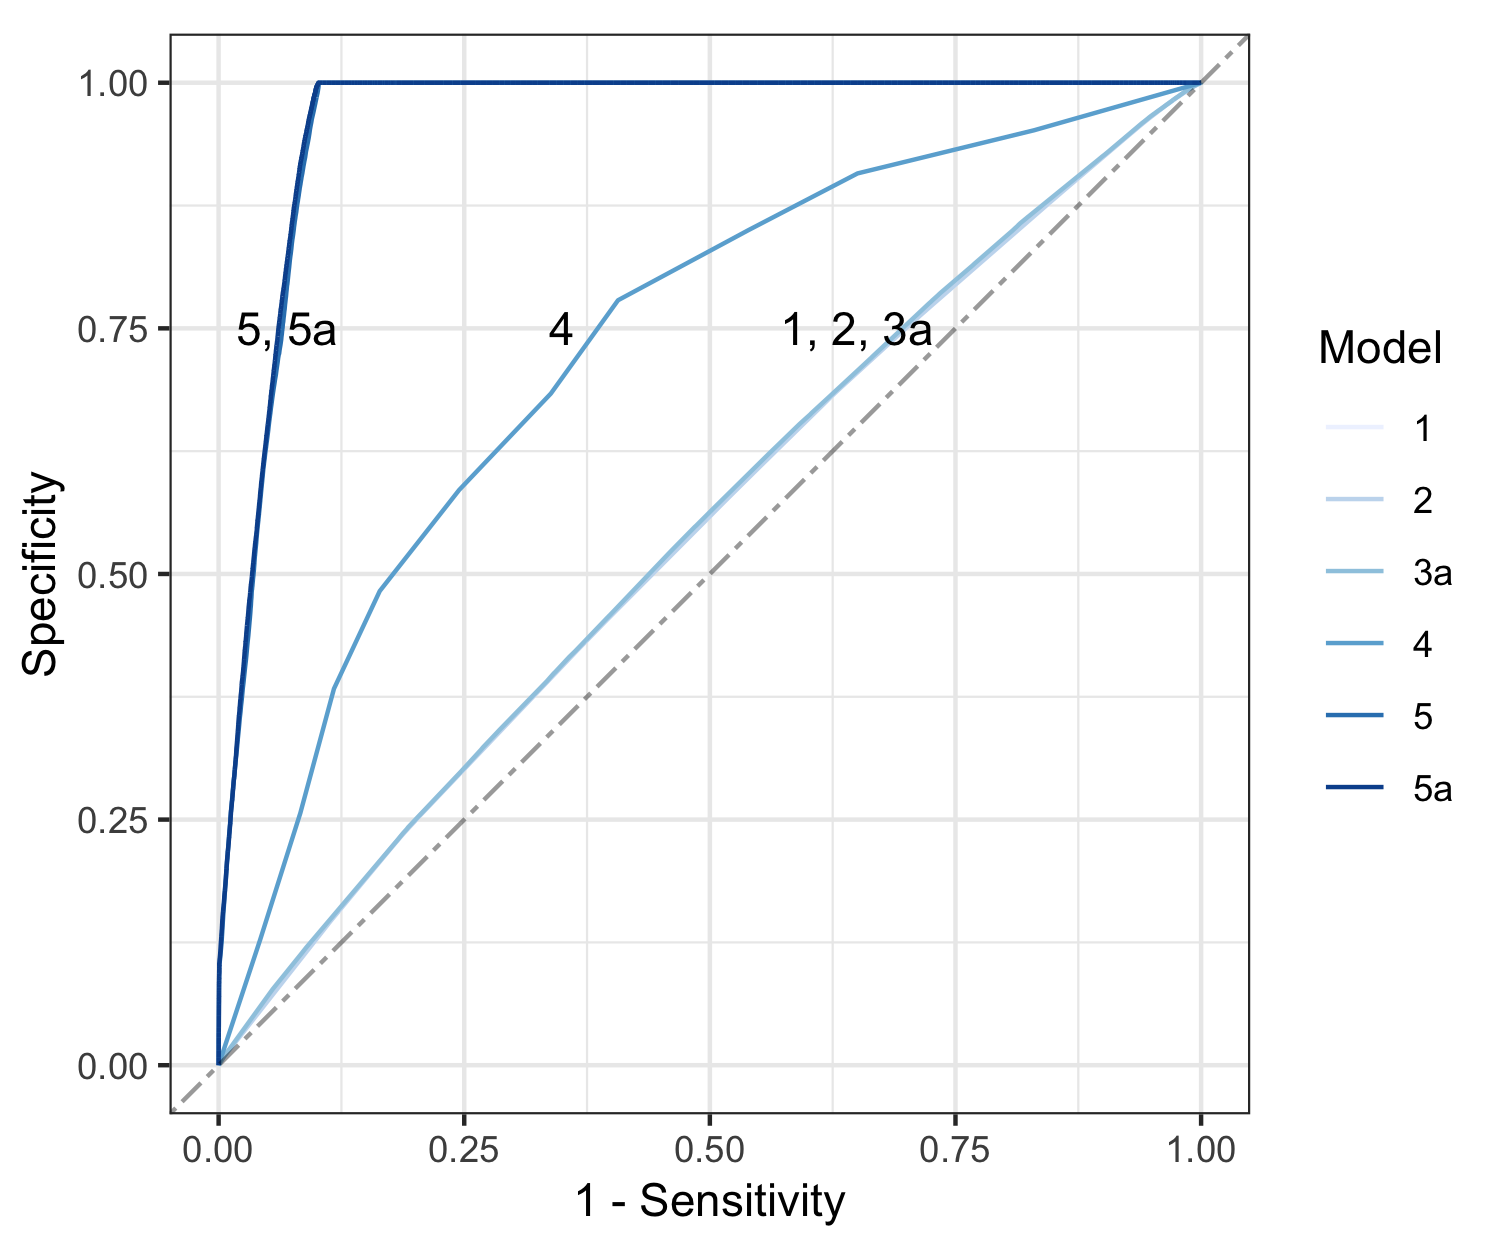
\includegraphics[width=0.6\linewidth]{/Users/tdounias/Desktop/Reed_Senior_Thesis/plots/roc_curves_indiv} 
  
  }
  
  \caption[ROC Curve for all individual models]{ROC Curve for all individual models}\label{fig:roc the curves}
  \end{figure}
  
  In terms of trusting these results, I am confident in the results of
  models 1 and 3a, somewhat confident in model 5, and less so for models
  2, 3, and 5a. Models 2, 3 and 5a ``failed to converge''; this means that
  the numeric approximation process by which \textit{R} implements maximum
  likelihood estimation\footnote{Estimation of maximum likelihood here
    uses Adaptive Gaussian-Hermitian Quadrature (AGQ) to estimate
    coefficients (Handayani, Notodiputro, Sadik, \& Kurnia, 2017)} for
  coefficients doesn't give stable results, within certain conditions.
  While model 5 did converge, it suffers from lack of variance in the
  predictor for VBM, as explained in the beginning of this chapter; this
  is the reason why the coefficient for mail vote is so disproportionately
  large and variable. Model 6 simply did not run, even on a re-sampled
  dataset. While I can't really derive any conclusions from this fact,
  there is a distinct possibility that this either occurred due to a lack
  of processing power, or lack of sufficient data for the model estimation
  to even reach close to convergence. It is also important to point out
  that model non-convergence is not a fatal issue in and of itself, but
  becomes so if outputted coefficients wildly differ between calls of the
  model. In this case, while running 5-fold cross validation for AUC, the
  coefficients remained fairly stable regardless of non-convergence.
  
  In terms of model fit, the models neatly fall into three groups based on
  their cross-validated AUC. The first group, consisting of models 1, 2,
  and 3a has an AUC of around \(.544\), making them only slightly
  distinguishable from a coin-toss. This is fairly reasonable, since I am
  building a model to make predictions at the ballot level while only
  using county data or gender\footnote{Few counties wildly differ in their
    turnout percentages, and that the coefficient for male gender results
    in only around a 2.5\% decrease in voting probability}. The second
  group based on AUC includes model 4, the only non-multilevel individual
  model, with an AUC of around \(.733\), significantly outperforming the
  first three models. Again, this is reasonable considering how wildly
  different turnout is between election types; it is only natural that
  these election-level variables would be so informative. The third group,
  with the highest AUC of around \(.96\) are models 5 and 5a. This is a
  direct result of the lack of variability in my data: Mail Voting is an
  almost perfect predictor of the probability of voting.
  
  There are two conclusions that can be derived from these results. None
  of these conclusions are, sadly, related to my hypotheses on VBM. The
  first is that the lack of variance in the data and a lack of processing
  power are direct causes of my inability to estimate these models. This
  is apparent in how model 6 does not run, other models do not converge,
  and the coefficient for VBM is very large, since it doesn't vary enough
  even after stratified sampling to account for any variance between mail
  vote and conventional ballots. The second conclusion here is that,
  despite these issues, there are some confirmable results on turnout in
  general that are common between individual and county models. For
  example, across models 2, 3, 3a the urban population of a county is a
  substantial, negative factor in probability of voting, while the white
  population is a very small, positive effect\footnote{This did, however,
    fail to reach statistical significance in both county and individual
    level models. This means that the small, positive effect is not that
    distinguishable from no effect at all.}. Same goes for male gender,
  which is a very small negative effect in voting probability as compared
  to female gender. These effects being stable across several models mean
  that they are independent of the additions to those models; for example,
  gender, urban population, and white population have effects that are not
  accounted for when adding individual level mixed effects. Despite not
  being able to assess VBM as a factor of turnout probability, these
  models at least show that the data does have substantial use for
  modelling at the individual level.
  
  \begin{longtable}[]{@{}lccccccc@{}}
  \caption{Estimated individual level coefficients
  \label{tab:model_indiv_coef}}\tabularnewline
  \toprule
  \begin{minipage}[b]{0.11\columnwidth}\raggedright\strut
  Predictor\strut
  \end{minipage} & \begin{minipage}[b]{0.08\columnwidth}\centering\strut
  Model 1\strut
  \end{minipage} & \begin{minipage}[b]{0.10\columnwidth}\centering\strut
  Model 2\strut
  \end{minipage} & \begin{minipage}[b]{0.10\columnwidth}\centering\strut
  Model 3\strut
  \end{minipage} & \begin{minipage}[b]{0.10\columnwidth}\centering\strut
  Model 3a\strut
  \end{minipage} & \begin{minipage}[b]{0.10\columnwidth}\centering\strut
  Model 4\strut
  \end{minipage} & \begin{minipage}[b]{0.10\columnwidth}\centering\strut
  Model 5\strut
  \end{minipage} & \begin{minipage}[b]{0.10\columnwidth}\centering\strut
  Model 5a\strut
  \end{minipage}\tabularnewline
  \midrule
  \endfirsthead
  \toprule
  \begin{minipage}[b]{0.11\columnwidth}\raggedright\strut
  Predictor\strut
  \end{minipage} & \begin{minipage}[b]{0.08\columnwidth}\centering\strut
  Model 1\strut
  \end{minipage} & \begin{minipage}[b]{0.10\columnwidth}\centering\strut
  Model 2\strut
  \end{minipage} & \begin{minipage}[b]{0.10\columnwidth}\centering\strut
  Model 3\strut
  \end{minipage} & \begin{minipage}[b]{0.10\columnwidth}\centering\strut
  Model 3a\strut
  \end{minipage} & \begin{minipage}[b]{0.10\columnwidth}\centering\strut
  Model 4\strut
  \end{minipage} & \begin{minipage}[b]{0.10\columnwidth}\centering\strut
  Model 5\strut
  \end{minipage} & \begin{minipage}[b]{0.10\columnwidth}\centering\strut
  Model 5a\strut
  \end{minipage}\tabularnewline
  \midrule
  \endhead
  \begin{minipage}[t]{0.11\columnwidth}\raggedright\strut
  (Intercept)\strut
  \end{minipage} & \begin{minipage}[t]{0.08\columnwidth}\centering\strut
  -0.175\strut
  \end{minipage} & \begin{minipage}[t]{0.10\columnwidth}\centering\strut
  -0.042\strut
  \end{minipage} & \begin{minipage}[t]{0.10\columnwidth}\centering\strut
  0.001\strut
  \end{minipage} & \begin{minipage}[t]{0.10\columnwidth}\centering\strut
  0.001\strut
  \end{minipage} & \begin{minipage}[t]{0.10\columnwidth}\centering\strut
  -0.541\strut
  \end{minipage} & \begin{minipage}[t]{0.10\columnwidth}\centering\strut
  -2.478\strut
  \end{minipage} & \begin{minipage}[t]{0.10\columnwidth}\centering\strut
  -1.888\strut
  \end{minipage}\tabularnewline
  \begin{minipage}[t]{0.11\columnwidth}\raggedright\strut
  \strut
  \end{minipage} & \begin{minipage}[t]{0.08\columnwidth}\centering\strut
  (0.030)\strut
  \end{minipage} & \begin{minipage}[t]{0.10\columnwidth}\centering\strut
  (0.083)\strut
  \end{minipage} & \begin{minipage}[t]{0.10\columnwidth}\centering\strut
  (0.060)\strut
  \end{minipage} & \begin{minipage}[t]{0.10\columnwidth}\centering\strut
  (0.076)\strut
  \end{minipage} & \begin{minipage}[t]{0.10\columnwidth}\centering\strut
  (0.009)**\strut
  \end{minipage} & \begin{minipage}[t]{0.10\columnwidth}\centering\strut
  (0.015)**\strut
  \end{minipage} & \begin{minipage}[t]{0.10\columnwidth}\centering\strut
  (0.238)**\strut
  \end{minipage}\tabularnewline
  \begin{minipage}[t]{0.11\columnwidth}\raggedright\strut
  Pct\_urban\strut
  \end{minipage} & \begin{minipage}[t]{0.08\columnwidth}\centering\strut
  \strut
  \end{minipage} & \begin{minipage}[t]{0.10\columnwidth}\centering\strut
  -0.423\strut
  \end{minipage} & \begin{minipage}[t]{0.10\columnwidth}\centering\strut
  -0.436\strut
  \end{minipage} & \begin{minipage}[t]{0.10\columnwidth}\centering\strut
  -0.424\strut
  \end{minipage} & \begin{minipage}[t]{0.10\columnwidth}\centering\strut
  \strut
  \end{minipage} & \begin{minipage}[t]{0.10\columnwidth}\centering\strut
  \strut
  \end{minipage} & \begin{minipage}[t]{0.10\columnwidth}\centering\strut
  -0.538\strut
  \end{minipage}\tabularnewline
  \begin{minipage}[t]{0.11\columnwidth}\raggedright\strut
  \strut
  \end{minipage} & \begin{minipage}[t]{0.08\columnwidth}\centering\strut
  \strut
  \end{minipage} & \begin{minipage}[t]{0.10\columnwidth}\centering\strut
  (0.055)**\strut
  \end{minipage} & \begin{minipage}[t]{0.10\columnwidth}\centering\strut
  (0.059)**\strut
  \end{minipage} & \begin{minipage}[t]{0.10\columnwidth}\centering\strut
  (0.062)**\strut
  \end{minipage} & \begin{minipage}[t]{0.10\columnwidth}\centering\strut
  \strut
  \end{minipage} & \begin{minipage}[t]{0.10\columnwidth}\centering\strut
  \strut
  \end{minipage} & \begin{minipage}[t]{0.10\columnwidth}\centering\strut
  (0.114)**\strut
  \end{minipage}\tabularnewline
  \begin{minipage}[t]{0.11\columnwidth}\raggedright\strut
  Pct\_white\strut
  \end{minipage} & \begin{minipage}[t]{0.08\columnwidth}\centering\strut
  \strut
  \end{minipage} & \begin{minipage}[t]{0.10\columnwidth}\centering\strut
  0.067\strut
  \end{minipage} & \begin{minipage}[t]{0.10\columnwidth}\centering\strut
  0.075\strut
  \end{minipage} & \begin{minipage}[t]{0.10\columnwidth}\centering\strut
  0.073\strut
  \end{minipage} & \begin{minipage}[t]{0.10\columnwidth}\centering\strut
  \strut
  \end{minipage} & \begin{minipage}[t]{0.10\columnwidth}\centering\strut
  \strut
  \end{minipage} & \begin{minipage}[t]{0.10\columnwidth}\centering\strut
  -0.151\strut
  \end{minipage}\tabularnewline
  \begin{minipage}[t]{0.11\columnwidth}\raggedright\strut
  \strut
  \end{minipage} & \begin{minipage}[t]{0.08\columnwidth}\centering\strut
  \strut
  \end{minipage} & \begin{minipage}[t]{0.10\columnwidth}\centering\strut
  (0.102)\strut
  \end{minipage} & \begin{minipage}[t]{0.10\columnwidth}\centering\strut
  (0.073)\strut
  \end{minipage} & \begin{minipage}[t]{0.10\columnwidth}\centering\strut
  (0.094)\strut
  \end{minipage} & \begin{minipage}[t]{0.10\columnwidth}\centering\strut
  \strut
  \end{minipage} & \begin{minipage}[t]{0.10\columnwidth}\centering\strut
  \strut
  \end{minipage} & \begin{minipage}[t]{0.10\columnwidth}\centering\strut
  (0.281)\strut
  \end{minipage}\tabularnewline
  \begin{minipage}[t]{0.11\columnwidth}\raggedright\strut
  genderMale\strut
  \end{minipage} & \begin{minipage}[t]{0.08\columnwidth}\centering\strut
  \strut
  \end{minipage} & \begin{minipage}[t]{0.10\columnwidth}\centering\strut
  \strut
  \end{minipage} & \begin{minipage}[t]{0.10\columnwidth}\centering\strut
  -0.097\strut
  \end{minipage} & \begin{minipage}[t]{0.10\columnwidth}\centering\strut
  -0.094\strut
  \end{minipage} & \begin{minipage}[t]{0.10\columnwidth}\centering\strut
  \strut
  \end{minipage} & \begin{minipage}[t]{0.10\columnwidth}\centering\strut
  \strut
  \end{minipage} & \begin{minipage}[t]{0.10\columnwidth}\centering\strut
  0.094\strut
  \end{minipage}\tabularnewline
  \begin{minipage}[t]{0.11\columnwidth}\raggedright\strut
  \strut
  \end{minipage} & \begin{minipage}[t]{0.08\columnwidth}\centering\strut
  \strut
  \end{minipage} & \begin{minipage}[t]{0.10\columnwidth}\centering\strut
  \strut
  \end{minipage} & \begin{minipage}[t]{0.10\columnwidth}\centering\strut
  (0.007)**\strut
  \end{minipage} & \begin{minipage}[t]{0.10\columnwidth}\centering\strut
  (0.007)**\strut
  \end{minipage} & \begin{minipage}[t]{0.10\columnwidth}\centering\strut
  \strut
  \end{minipage} & \begin{minipage}[t]{0.10\columnwidth}\centering\strut
  \strut
  \end{minipage} & \begin{minipage}[t]{0.10\columnwidth}\centering\strut
  (0.017)**\strut
  \end{minipage}\tabularnewline
  \begin{minipage}[t]{0.11\columnwidth}\raggedright\strut
  Republican\strut
  \end{minipage} & \begin{minipage}[t]{0.08\columnwidth}\centering\strut
  \strut
  \end{minipage} & \begin{minipage}[t]{0.10\columnwidth}\centering\strut
  \strut
  \end{minipage} & \begin{minipage}[t]{0.10\columnwidth}\centering\strut
  \strut
  \end{minipage} & \begin{minipage}[t]{0.10\columnwidth}\centering\strut
  \strut
  \end{minipage} & \begin{minipage}[t]{0.10\columnwidth}\centering\strut
  \strut
  \end{minipage} & \begin{minipage}[t]{0.10\columnwidth}\centering\strut
  0.233\strut
  \end{minipage} & \begin{minipage}[t]{0.10\columnwidth}\centering\strut
  0.208\strut
  \end{minipage}\tabularnewline
  \begin{minipage}[t]{0.11\columnwidth}\raggedright\strut
  \strut
  \end{minipage} & \begin{minipage}[t]{0.08\columnwidth}\centering\strut
  \strut
  \end{minipage} & \begin{minipage}[t]{0.10\columnwidth}\centering\strut
  \strut
  \end{minipage} & \begin{minipage}[t]{0.10\columnwidth}\centering\strut
  \strut
  \end{minipage} & \begin{minipage}[t]{0.10\columnwidth}\centering\strut
  \strut
  \end{minipage} & \begin{minipage}[t]{0.10\columnwidth}\centering\strut
  \strut
  \end{minipage} & \begin{minipage}[t]{0.10\columnwidth}\centering\strut
  (0.021)**\strut
  \end{minipage} & \begin{minipage}[t]{0.10\columnwidth}\centering\strut
  (0.073)**\strut
  \end{minipage}\tabularnewline
  \begin{minipage}[t]{0.11\columnwidth}\raggedright\strut
  Other\strut
  \end{minipage} & \begin{minipage}[t]{0.08\columnwidth}\centering\strut
  \strut
  \end{minipage} & \begin{minipage}[t]{0.10\columnwidth}\centering\strut
  \strut
  \end{minipage} & \begin{minipage}[t]{0.10\columnwidth}\centering\strut
  \strut
  \end{minipage} & \begin{minipage}[t]{0.10\columnwidth}\centering\strut
  \strut
  \end{minipage} & \begin{minipage}[t]{0.10\columnwidth}\centering\strut
  \strut
  \end{minipage} & \begin{minipage}[t]{0.10\columnwidth}\centering\strut
  -0.085\strut
  \end{minipage} & \begin{minipage}[t]{0.10\columnwidth}\centering\strut
  -0.124\strut
  \end{minipage}\tabularnewline
  \begin{minipage}[t]{0.11\columnwidth}\raggedright\strut
  \strut
  \end{minipage} & \begin{minipage}[t]{0.08\columnwidth}\centering\strut
  \strut
  \end{minipage} & \begin{minipage}[t]{0.10\columnwidth}\centering\strut
  \strut
  \end{minipage} & \begin{minipage}[t]{0.10\columnwidth}\centering\strut
  \strut
  \end{minipage} & \begin{minipage}[t]{0.10\columnwidth}\centering\strut
  \strut
  \end{minipage} & \begin{minipage}[t]{0.10\columnwidth}\centering\strut
  \strut
  \end{minipage} & \begin{minipage}[t]{0.10\columnwidth}\centering\strut
  (0.073)\strut
  \end{minipage} & \begin{minipage}[t]{0.10\columnwidth}\centering\strut
  (0.073)\strut
  \end{minipage}\tabularnewline
  \begin{minipage}[t]{0.11\columnwidth}\raggedright\strut
  UAF\strut
  \end{minipage} & \begin{minipage}[t]{0.08\columnwidth}\centering\strut
  \strut
  \end{minipage} & \begin{minipage}[t]{0.10\columnwidth}\centering\strut
  \strut
  \end{minipage} & \begin{minipage}[t]{0.10\columnwidth}\centering\strut
  \strut
  \end{minipage} & \begin{minipage}[t]{0.10\columnwidth}\centering\strut
  \strut
  \end{minipage} & \begin{minipage}[t]{0.10\columnwidth}\centering\strut
  \strut
  \end{minipage} & \begin{minipage}[t]{0.10\columnwidth}\centering\strut
  -0.308\strut
  \end{minipage} & \begin{minipage}[t]{0.10\columnwidth}\centering\strut
  0.325\strut
  \end{minipage}\tabularnewline
  \begin{minipage}[t]{0.11\columnwidth}\raggedright\strut
  \strut
  \end{minipage} & \begin{minipage}[t]{0.08\columnwidth}\centering\strut
  \strut
  \end{minipage} & \begin{minipage}[t]{0.10\columnwidth}\centering\strut
  \strut
  \end{minipage} & \begin{minipage}[t]{0.10\columnwidth}\centering\strut
  \strut
  \end{minipage} & \begin{minipage}[t]{0.10\columnwidth}\centering\strut
  \strut
  \end{minipage} & \begin{minipage}[t]{0.10\columnwidth}\centering\strut
  \strut
  \end{minipage} & \begin{minipage}[t]{0.10\columnwidth}\centering\strut
  (0.021)**\strut
  \end{minipage} & \begin{minipage}[t]{0.10\columnwidth}\centering\strut
  (0.021)**\strut
  \end{minipage}\tabularnewline
  \begin{minipage}[t]{0.11\columnwidth}\raggedright\strut
  VBM\strut
  \end{minipage} & \begin{minipage}[t]{0.08\columnwidth}\centering\strut
  \strut
  \end{minipage} & \begin{minipage}[t]{0.10\columnwidth}\centering\strut
  \strut
  \end{minipage} & \begin{minipage}[t]{0.10\columnwidth}\centering\strut
  \strut
  \end{minipage} & \begin{minipage}[t]{0.10\columnwidth}\centering\strut
  \strut
  \end{minipage} & \begin{minipage}[t]{0.10\columnwidth}\centering\strut
  \strut
  \end{minipage} & \begin{minipage}[t]{0.10\columnwidth}\centering\strut
  23.764\strut
  \end{minipage} & \begin{minipage}[t]{0.10\columnwidth}\centering\strut
  26.502\strut
  \end{minipage}\tabularnewline
  \begin{minipage}[t]{0.11\columnwidth}\raggedright\strut
  \strut
  \end{minipage} & \begin{minipage}[t]{0.08\columnwidth}\centering\strut
  \strut
  \end{minipage} & \begin{minipage}[t]{0.10\columnwidth}\centering\strut
  \strut
  \end{minipage} & \begin{minipage}[t]{0.10\columnwidth}\centering\strut
  \strut
  \end{minipage} & \begin{minipage}[t]{0.10\columnwidth}\centering\strut
  \strut
  \end{minipage} & \begin{minipage}[t]{0.10\columnwidth}\centering\strut
  \strut
  \end{minipage} & \begin{minipage}[t]{0.10\columnwidth}\centering\strut
  (45.255)**\strut
  \end{minipage} & \begin{minipage}[t]{0.10\columnwidth}\centering\strut
  (285.774)**\strut
  \end{minipage}\tabularnewline
  \begin{minipage}[t]{0.11\columnwidth}\raggedright\strut
  Age\strut
  \end{minipage} & \begin{minipage}[t]{0.08\columnwidth}\centering\strut
  \strut
  \end{minipage} & \begin{minipage}[t]{0.10\columnwidth}\centering\strut
  \strut
  \end{minipage} & \begin{minipage}[t]{0.10\columnwidth}\centering\strut
  \strut
  \end{minipage} & \begin{minipage}[t]{0.10\columnwidth}\centering\strut
  \strut
  \end{minipage} & \begin{minipage}[t]{0.10\columnwidth}\centering\strut
  \strut
  \end{minipage} & \begin{minipage}[t]{0.10\columnwidth}\centering\strut
  0.093\strut
  \end{minipage} & \begin{minipage}[t]{0.10\columnwidth}\centering\strut
  0.086\strut
  \end{minipage}\tabularnewline
  \begin{minipage}[t]{0.11\columnwidth}\raggedright\strut
  \strut
  \end{minipage} & \begin{minipage}[t]{0.08\columnwidth}\centering\strut
  \strut
  \end{minipage} & \begin{minipage}[t]{0.10\columnwidth}\centering\strut
  \strut
  \end{minipage} & \begin{minipage}[t]{0.10\columnwidth}\centering\strut
  \strut
  \end{minipage} & \begin{minipage}[t]{0.10\columnwidth}\centering\strut
  \strut
  \end{minipage} & \begin{minipage}[t]{0.10\columnwidth}\centering\strut
  \strut
  \end{minipage} & \begin{minipage}[t]{0.10\columnwidth}\centering\strut
  (0.009)**\strut
  \end{minipage} & \begin{minipage}[t]{0.10\columnwidth}\centering\strut
  (0.009)**\strut
  \end{minipage}\tabularnewline
  \begin{minipage}[t]{0.11\columnwidth}\raggedright\strut
  typeGeneral\strut
  \end{minipage} & \begin{minipage}[t]{0.08\columnwidth}\centering\strut
  \strut
  \end{minipage} & \begin{minipage}[t]{0.10\columnwidth}\centering\strut
  \strut
  \end{minipage} & \begin{minipage}[t]{0.10\columnwidth}\centering\strut
  \strut
  \end{minipage} & \begin{minipage}[t]{0.10\columnwidth}\centering\strut
  \strut
  \end{minipage} & \begin{minipage}[t]{0.10\columnwidth}\centering\strut
  1.537\strut
  \end{minipage} & \begin{minipage}[t]{0.10\columnwidth}\centering\strut
  \strut
  \end{minipage} & \begin{minipage}[t]{0.10\columnwidth}\centering\strut
  \strut
  \end{minipage}\tabularnewline
  \begin{minipage}[t]{0.11\columnwidth}\raggedright\strut
  \strut
  \end{minipage} & \begin{minipage}[t]{0.08\columnwidth}\centering\strut
  \strut
  \end{minipage} & \begin{minipage}[t]{0.10\columnwidth}\centering\strut
  \strut
  \end{minipage} & \begin{minipage}[t]{0.10\columnwidth}\centering\strut
  \strut
  \end{minipage} & \begin{minipage}[t]{0.10\columnwidth}\centering\strut
  \strut
  \end{minipage} & \begin{minipage}[t]{0.10\columnwidth}\centering\strut
  (0.011)**\strut
  \end{minipage} & \begin{minipage}[t]{0.10\columnwidth}\centering\strut
  \strut
  \end{minipage} & \begin{minipage}[t]{0.10\columnwidth}\centering\strut
  \strut
  \end{minipage}\tabularnewline
  \begin{minipage}[t]{0.11\columnwidth}\raggedright\strut
  typeMidterm\strut
  \end{minipage} & \begin{minipage}[t]{0.08\columnwidth}\centering\strut
  \strut
  \end{minipage} & \begin{minipage}[t]{0.10\columnwidth}\centering\strut
  \strut
  \end{minipage} & \begin{minipage}[t]{0.10\columnwidth}\centering\strut
  \strut
  \end{minipage} & \begin{minipage}[t]{0.10\columnwidth}\centering\strut
  \strut
  \end{minipage} & \begin{minipage}[t]{0.10\columnwidth}\centering\strut
  0.829\strut
  \end{minipage} & \begin{minipage}[t]{0.10\columnwidth}\centering\strut
  \strut
  \end{minipage} & \begin{minipage}[t]{0.10\columnwidth}\centering\strut
  \strut
  \end{minipage}\tabularnewline
  \begin{minipage}[t]{0.11\columnwidth}\raggedright\strut
  \strut
  \end{minipage} & \begin{minipage}[t]{0.08\columnwidth}\centering\strut
  \strut
  \end{minipage} & \begin{minipage}[t]{0.10\columnwidth}\centering\strut
  \strut
  \end{minipage} & \begin{minipage}[t]{0.10\columnwidth}\centering\strut
  \strut
  \end{minipage} & \begin{minipage}[t]{0.10\columnwidth}\centering\strut
  \strut
  \end{minipage} & \begin{minipage}[t]{0.10\columnwidth}\centering\strut
  (0.011)**\strut
  \end{minipage} & \begin{minipage}[t]{0.10\columnwidth}\centering\strut
  \strut
  \end{minipage} & \begin{minipage}[t]{0.10\columnwidth}\centering\strut
  \strut
  \end{minipage}\tabularnewline
  \begin{minipage}[t]{0.11\columnwidth}\raggedright\strut
  typePrimary\strut
  \end{minipage} & \begin{minipage}[t]{0.08\columnwidth}\centering\strut
  \strut
  \end{minipage} & \begin{minipage}[t]{0.10\columnwidth}\centering\strut
  \strut
  \end{minipage} & \begin{minipage}[t]{0.10\columnwidth}\centering\strut
  \strut
  \end{minipage} & \begin{minipage}[t]{0.10\columnwidth}\centering\strut
  \strut
  \end{minipage} & \begin{minipage}[t]{0.10\columnwidth}\centering\strut
  -0.880\strut
  \end{minipage} & \begin{minipage}[t]{0.10\columnwidth}\centering\strut
  \strut
  \end{minipage} & \begin{minipage}[t]{0.10\columnwidth}\centering\strut
  \strut
  \end{minipage}\tabularnewline
  \begin{minipage}[t]{0.11\columnwidth}\raggedright\strut
  \strut
  \end{minipage} & \begin{minipage}[t]{0.08\columnwidth}\centering\strut
  \strut
  \end{minipage} & \begin{minipage}[t]{0.10\columnwidth}\centering\strut
  \strut
  \end{minipage} & \begin{minipage}[t]{0.10\columnwidth}\centering\strut
  \strut
  \end{minipage} & \begin{minipage}[t]{0.10\columnwidth}\centering\strut
  \strut
  \end{minipage} & \begin{minipage}[t]{0.10\columnwidth}\centering\strut
  (0.010)**\strut
  \end{minipage} & \begin{minipage}[t]{0.10\columnwidth}\centering\strut
  \strut
  \end{minipage} & \begin{minipage}[t]{0.10\columnwidth}\centering\strut
  \strut
  \end{minipage}\tabularnewline
  \begin{minipage}[t]{0.11\columnwidth}\raggedright\strut
  CV AUC\strut
  \end{minipage} & \begin{minipage}[t]{0.08\columnwidth}\centering\strut
  0.543\strut
  \end{minipage} & \begin{minipage}[t]{0.10\columnwidth}\centering\strut
  0.543\strut
  \end{minipage} & \begin{minipage}[t]{0.10\columnwidth}\centering\strut
  \strut
  \end{minipage} & \begin{minipage}[t]{0.10\columnwidth}\centering\strut
  0.545\strut
  \end{minipage} & \begin{minipage}[t]{0.10\columnwidth}\centering\strut
  0.733\strut
  \end{minipage} & \begin{minipage}[t]{0.10\columnwidth}\centering\strut
  0.961\strut
  \end{minipage} & \begin{minipage}[t]{0.10\columnwidth}\centering\strut
  0.963\strut
  \end{minipage}\tabularnewline
  \begin{minipage}[t]{0.11\columnwidth}\raggedright\strut
  Obs\strut
  \end{minipage} & \begin{minipage}[t]{0.08\columnwidth}\centering\strut
  370,586\strut
  \end{minipage} & \begin{minipage}[t]{0.10\columnwidth}\centering\strut
  370,586\strut
  \end{minipage} & \begin{minipage}[t]{0.10\columnwidth}\centering\strut
  370,586\strut
  \end{minipage} & \begin{minipage}[t]{0.10\columnwidth}\centering\strut
  370,586\strut
  \end{minipage} & \begin{minipage}[t]{0.10\columnwidth}\centering\strut
  370,586\strut
  \end{minipage} & \begin{minipage}[t]{0.10\columnwidth}\centering\strut
  370,586\strut
  \end{minipage} & \begin{minipage}[t]{0.10\columnwidth}\centering\strut
  370,586\strut
  \end{minipage}\tabularnewline
  \begin{minipage}[t]{0.11\columnwidth}\raggedright\strut
  Groups\strut
  \end{minipage} & \begin{minipage}[t]{0.08\columnwidth}\centering\strut
  64\strut
  \end{minipage} & \begin{minipage}[t]{0.10\columnwidth}\centering\strut
  64\strut
  \end{minipage} & \begin{minipage}[t]{0.10\columnwidth}\centering\strut
  64\strut
  \end{minipage} & \begin{minipage}[t]{0.10\columnwidth}\centering\strut
  64\strut
  \end{minipage} & \begin{minipage}[t]{0.10\columnwidth}\centering\strut
  64\strut
  \end{minipage} & \begin{minipage}[t]{0.10\columnwidth}\centering\strut
  64\strut
  \end{minipage} & \begin{minipage}[t]{0.10\columnwidth}\centering\strut
  64\strut
  \end{minipage}\tabularnewline
  \bottomrule
  \end{longtable}
  
  \chapter*{Conclusion}\label{conclusion}
  \addcontentsline{toc}{chapter}{Conclusion}
  
  \setcounter{chapter}{5} \setcounter{section}{0}
  
  At the end of the day I am unable to draw concrete conclusions on my
  hypotheses. My county level models do provide some indication that my
  second and third hypotheses (H2,H3)--relating to stronger VBM effects on
  lower level elections--is probably false for Colorado, when comparing
  general elections to primaries or coordinated local races. I do not
  however draw conclusions on my first hypothesis; while it seems that the
  effect of mail voting is present, and consistent through time, it
  doesn't seem like this effect is particularly different from any other
  effects like urban population. I would say that this is weak evidence in
  favor of H1, but not enough to solidly confirm it.
  
  Resulting from this, the main contribution of my thesis has to be in
  analysis of data wrangling, the construction of multilevel general
  additive models for turnout, and the accompanying \textit{R} package. To
  take these one by one, I have provided arguments in favor of preferring
  multiple snapshots of registration files rather than just the latest
  iteration of the record. I have analyzed the pitfalls that exist in such
  documents, and given specific examples on how this can be dealt with for
  the Colorado data files. I have also provided a set of variable
  specification that can be useful as indicators of the content of these
  data, or the potential uses of voter registration files in other future
  studies. Finally, I have presented potential future solutions to issues
  these data have with variability, and ways to circumvent processing
  power limitations.
  
  Additionally, I have meticulously gone through the creation of
  multilevel general additive models of individual and county level
  turnout. While due to data and processing power limitations I am unable
  to run all these models. this does not mean that they present no value
  to future research. Quite the contrary, they aid in future studies just
  having to go through the data clean-up stage, and then implement my
  models without having to construct them from scratch. In particular,
  mixed effects and general additive models are not widely used in such
  studies, making their presentation and specification rather unique
  regardless of their application in this piece of research.
  
  Lastly, I provide an extensive library of code used to create this
  document and the research I conduct. I have made an \textit{R}
  package--which I named \texttt{riggd}--that includes more than a dozen
  different functions that serve data wrangling and presentation purposes.
  These functions are made for use on Colorado files, but require
  relatively small amounts of changes to be applied to voter files from
  around the US. I also provide code for all tables and graphics that are
  included in this thesis on gitHub, which is a testament to the
  reproducibility and future value of the research I conducted.
  
  I recognize that, despite many obstacles in terms of data or computing
  power, the outcome of this thesis being more constructive rather than
  conclusive is to some extent my fault. There were many problems in this
  thesis that I should have been aware of earlier in the process, which
  may have allowed me to present some concrete result rather than a series
  of tools and methods. However, in the combination of my existing
  conclusions and the materials I have created through this process, it is
  my belief that this thesis does in fact present a step forward in the
  literature, and that it adds to existing quantitative elections studies
  works. This is a small step, but it helps in our understanding of how
  the franchise of democracy governs itself, and what the actual results
  of elections policy are.
  
  \appendix
  
  \backmatter
  
  \chapter{References}\label{references}
  
  \noindent
  
  \setlength{\parindent}{-0.20in} \setlength{\leftskip}{0.20in}
  \setlength{\parskip}{8pt}
  
  \hypertarget{refs}{}
  \hypertarget{ref-aldrich_rational_1993}{}
  Aldrich, J. H. (1993). Rational Choice and Turnout. \emph{American
  Journal of Political Science}, \emph{37}(1), 246--278.
  \url{http://doi.org/10.2307/2111531}
  
  \hypertarget{ref-ansolabehere_quality_2010}{}
  Ansolabehere, S., \& Hersh, E. (2010). The Quality of Voter Registration
  Records: A State-by-State Analysis. \emph{Institute for Quantitative
  Social Science and Caltech/MIT Voting Technology Project Working Paper}.
  Retrieved from
  \url{https://dataverse.harvard.edu/dataset.xhtml?persistentId=hdl:1902.1/18550}
  
  \hypertarget{ref-ansolabehere_validation:_2012}{}
  Ansolabehere, S., \& Hersh, E. (2012). Validation: What Big Data Reveal
  About Survey Misreporting and the Real Electorate. \emph{Political
  Analysis}, \emph{20}(04), 437--459.
  \url{http://doi.org/10.1093/pan/mps023}
  
  \hypertarget{ref-ansolabehere_adgn:_2017}{}
  Ansolabehere, S., \& Hersh, E. D. (2017). ADGN: An Algorithm for Record
  Linkage Using Address, Date of Birth, Gender, and Name. \emph{Statistics
  and Public Policy}, \emph{4}(1), 1--10.
  \url{http://doi.org/10.1080/2330443X.2017.1389620}
  
  \hypertarget{ref-colorado_general_assembly_tabor_nodate}{}
  Assembly, C. G. (n.d.). TABOR. \emph{Colorado General Assembly}.
  Retrieved from
  \url{https://public.tableau.com/views/TABOR/TABORDash?:showVizHome=no:embed=y\&:display_count=no}
  
  \hypertarget{ref-barr_comprehensive_2012}{}
  Barr, C. D., Diez, D. M., Wang, Y., Dominici, F., \& Samet, J. M.
  (2012). Comprehensive Smoking Bans and Acute Myocardial Infarction Among
  Medicare Enrollees in 387 US Counties: 1999--2008. \emph{American
  Journal of Epidemiology}, \emph{176}(7), 642--648.
  \url{http://doi.org/10.1093/aje/kws267}
  
  \hypertarget{ref-bates_fitting_2014}{}
  Bates, D., Mächler, M., Bolker, B., \& Walker, S. (2014). Fitting Linear
  Mixed-Effects Models using lme4. \emph{arXiv:1406.5823 {[}Stat{]}}.
  Retrieved from \url{http://arxiv.org/abs/1406.5823}
  
  \hypertarget{ref-bergman_changing_2011}{}
  Bergman, E., \& Yates, P. A. (2011). Changing Election Methods: How Does
  Mandated Vote-By-Mail Affect Individual Registrants? \emph{Election Law
  Journal: Rules, Politics, and Policy}, \emph{10}(2), 115--127.
  \url{http://doi.org/10.1089/elj.2010.0079}
  
  \hypertarget{ref-berinsky_perverse_2005}{}
  Berinsky, A. J. (2005). The Perverse Consequences of Electoral Reform in
  the United States. \emph{American Politics Research}, \emph{33}(4),
  471--491. \url{http://doi.org/10.1177/1532673X04269419}
  
  \hypertarget{ref-burden_voter_2000}{}
  Burden, B. C. (2000). Voter Turnout and the National Election Studies.
  \emph{Political Analysis}, \emph{8}(4), 389--398.
  \url{http://doi.org/10.1093/oxfordjournals.pan.a029823}
  
  \hypertarget{ref-burden_new_1998}{}
  Burden, B. C., \& Kimball, D. C. (1998). A New Approach to the Study of
  Ticket Splitting. \emph{The American Political Science Review},
  \emph{92}(3), 533--544. \url{http://doi.org/10.2307/2585479}
  
  \hypertarget{ref-burden_election_2013}{}
  Burden, B. C., \& Neiheisel, J. R. (2013). Election Administration and
  the Pure Effect of Voter Registration on Turnout. \emph{Political
  Research Quarterly}, \emph{66}(1), 77--90.
  \url{http://doi.org/10.1177/1065912911430671}
  
  \hypertarget{ref-burden_election_2014}{}
  Burden, B. C., Canon, D. T., Mayer, K. R., \& Moynihan, D. P. (2014).
  Election Laws, Mobilization, and Turnout: The Unanticipated Consequences
  of Election Reform. \emph{American Journal of Political Science},
  \emph{58}(1), 95--109. \url{http://doi.org/10.1111/ajps.12063}
  
  \hypertarget{ref-us_census_bureau_us_2010}{}
  Bureau, U. C. (2010). US Census Bureau QuickFacts: Colorado. Retrieved
  from \url{https://www.census.gov/quickfacts/co}
  
  \hypertarget{ref-campbell_self-interest_2002}{}
  Campbell, A. L. (2002). Self-Interest, Social Security, and the
  Distinctive Participation Patterns of Senior Citizens. \emph{American
  Political Science Review}, \emph{96}(3), 565--574.
  \url{http://doi.org/10.1017/S0003055402000333}
  
  \hypertarget{ref-chen_voter_2013}{}
  Chen, J. (2013). Voter Partisanship and the Effect of Distributive
  Spending on Political Participation. \emph{American Journal of Political
  Science}, \emph{57}(1), 200--217.
  \url{http://doi.org/10.1111/j.1540-5907.2012.00613.x}
  
  \hypertarget{ref-chihara_mathematical_2011}{}
  Chihara, L. M., \& Hesterberg, T. C. (2011). \emph{Mathematical
  Statistics with Resampling and R} (1 edition). Hoboken, N.J: Wiley.
  
  \hypertarget{ref-cronin_colorado_2012}{}
  Cronin, T. E., \& Loevy, R. D. (2012). \emph{Colorado Politics and
  Policy: Governing a Purple State}. Lincoln, UNITED STATES: UNP -
  Nebraska Paperback. Retrieved from
  \url{http://ebookcentral.proquest.com/lib/reed/detail.action?docID=1034959}
  
  \hypertarget{ref-deufel_race_2010}{}
  Deufel, B. J., \& Kedar, O. (2010). Race And Turnout In U.S. Elections
  Exposing Hidden Effects. \emph{Public Opinion Quarterly}, \emph{74}(2),
  286--318. \url{http://doi.org/10.1093/poq/nfq017}
  
  \hypertarget{ref-edelman_analysis_2018}{}
  Edelman, G., \& Glastris, P. (2018). Analysis Letting people vote at
  home increases voter turnout. Here's proof. \emph{Washington Post}.
  Retrieved from
  \url{https://www.washingtonpost.com/outlook/letting-people-vote-at-home-increases-voter-turnout-heres-proof/2018/01/26/d637b9d2-017a-11e8-bb03-722769454f82_story.html}
  
  \hypertarget{ref-edlin_voting_2007}{}
  Edlin, A., Gelman, A., \& Kaplan, N. (2007). Voting as a Rational
  Choice: Why and How People Vote To Improve the Well-Being of Others.
  \emph{Rationality and Society}, \emph{19}(3), 293--314.
  \url{http://doi.org/10.1177/1043463107077384}
  
  \hypertarget{ref-ewald_way_2009}{}
  Ewald, A. C. (2009). \emph{The Way We Vote: The Local Dimension of
  American Suffrage}. Nashville: Vanderbilt University Press.
  
  \hypertarget{ref-fortier_absentee_2006}{}
  Fortier, J. C. (2006). \emph{Absentee and early voting: Trends,
  promises, and perils}. Washington, DC: AEI Press.
  
  \hypertarget{ref-fowler_habitual_2006}{}
  Fowler, J. H. (2006). Habitual Voting and Behavioral Turnout.
  \emph{Journal of Politics}, \emph{68}(2), 335--344.
  \url{http://doi.org/10.1111/j.1468-2508.2006.00410.x}
  
  \hypertarget{ref-gelman_data_2006}{}
  Gelman, A., \& Hill, J. (2006). \emph{Data Analysis Using Regression and
  Multilevel/Hierarchical Models} (1 edition). Cambridge ; New York:
  Cambridge University Press.
  
  \hypertarget{ref-gerber_identifying_2013}{}
  Gerber, A. S., Huber, G. A., \& Hill, S. J. (2013). Identifying the
  Effect of All-Mail Elections on Turnout: Staggered Reform in the
  Evergreen State\textless{}a
  href=``\#fn2606''\textgreater{}*\textless{}/a\textgreater{}.
  \emph{Political Science Research and Methods}, \emph{1}(1), 91--116.
  \url{http://doi.org/10.1017/psrm.2013.5}
  
  \hypertarget{ref-geys_explaining_2006}{}
  Geys, B. (2006). Explaining voter turnout: A review of aggregate-level
  research. \emph{Electoral Studies}, \emph{25}(4), 637--663.
  \url{http://doi.org/10.1016/j.electstud.2005.09.002}
  
  \hypertarget{ref-gronke_voting_2012}{}
  Gronke, P., \& Miller, P. (2012). Voting by Mail and Turnout in Oregon:
  Revisiting Southwell and Burchett. \emph{American Politics Research},
  \emph{40}(6), 976--997. \url{http://doi.org/10.1177/1532673X12457809}
  
  \hypertarget{ref-gronke_convenience_2008}{}
  Gronke, P., Galanes-Rosenbaum, E., Miller, P. A., \& Toffey, D. (2008).
  Convenience Voting. \emph{Annual Review of Political Science},
  \emph{11}(1), 437--455.
  \url{http://doi.org/10.1146/annurev.polisci.11.053006.190912}
  
  \hypertarget{ref-gronke_voter_2017}{}
  Gronke, P., McGhee, E., Romero, M., \& Griffin, R. (2017).
  Voter~~Registration~~and~~Turnout~~under
  ``Oregon~~Motor~~Voter'':~~A~~Second~~Look. In. Portland, OR. Retrieved
  from
  \url{https://dl.dropboxusercontent.com/nativeprint?file=https\%3A\%2F\%2Fwww.dropbox.com\%2Fs\%2Fo63a0zi7j8plhgl\%2FOMV_and_Turnout_McGhee_Gronke_Romero_Griffin_July2017.pdf\%3Fdisable_range\%3D1\%26from_native_print\%3D1\%26preview\%3D1}
  
  \hypertarget{ref-hamm_how_2017}{}
  Hamm, K. (2017). How Colorado has voted in presidential elections (and
  how its politics have changed) since 1980. \emph{The Denver Post}.
  Retrieved from
  \url{https://www.denverpost.com/2017/12/22/how-colorado-votes/}
  
  \hypertarget{ref-handayani_comparative_2017}{}
  Handayani, D., Notodiputro, K. A., Sadik, K., \& Kurnia, A. (2017). A
  comparative study of approximation methods for maximum likelihood
  estimation in generalized linear mixed models (GLMM). In (p. 020033).
  Jawa Barat, Indonesia. \url{http://doi.org/10.1063/1.4979449}
  
  \hypertarget{ref-hersh_hacking_2015}{}
  Hersh, E. D. (2015). \emph{Hacking the Electorate: How Campaigns
  Perceive Voters}. New York, NY: Cambridge University Press.
  
  \hypertarget{ref-hullinghorst_voter_2013}{}
  Hullinghorst, D. L., \& Pabon, D. (2013, May). Voter Access and
  Moderninzed Elections Act.
  
  \hypertarget{ref-james_introduction_2017}{}
  James, G., Witten, D., Hastie, T., \& Tibshirani, R. (2017). \emph{An
  Introduction to Statistical Learning: With Applications in R} (1st ed.
  2013, Corr. 7th printing 2017 edition). New York: Springer.
  
  \hypertarget{ref-keele_geographic_2017}{}
  Keele, L., \& Titiunik, R. (2017). Geographic Natural Experiments with
  Interference: The Effect of All-Mail Voting on Turnout in Colorado.
  
  \hypertarget{ref-martin_colorado_1962}{}
  Martin, C. (1962). \emph{Colorado politics} (2ond ed.). Denver,
  Colorado: Big Mountain Press. Retrieved from
  \url{http://hdl.handle.net/2027/mdp.39015024371158}
  
  \hypertarget{ref-matsusaka_voter_1999}{}
  Matsusaka, J. G., \& Palda, F. (1999). Voter turnout: How much can we
  explain? \emph{Public Choice}, \emph{98}(3-4), 431--446.
  \url{http://doi.org/10.1023/A:1018328621580}
  
  \hypertarget{ref-mcclelland_synthetic_2017}{}
  McClelland, R., \& Gault, S. (2017). The Synthetic Control Method as a
  Tool to Understand State Policy. \emph{Washington, DC: Urban-Brookings
  Tax Policy Center}.
  
  \hypertarget{ref-mcdonald_true_2007}{}
  Mcdonald, M. P. (2007). The True ElectorateA Cross-Validation of Voter
  Registration Files and Election Survey Demographics. \emph{Public
  Opinion Quarterly}, \emph{71}(4), 588--602.
  \url{http://doi.org/10.1093/poq/nfm046}
  
  \hypertarget{ref-mettler_government_2008}{}
  Mettler, S., \& Stonecash, J. M. (2008). Government Program Usage and
  Political Voice*. \emph{Social Science Quarterly}, \emph{89}(2),
  273--293. \url{http://doi.org/10.1111/j.1540-6237.2008.00532.x}
  
  \hypertarget{ref-neiheisel_impact_2012}{}
  Neiheisel, J. R., \& Burden, B. C. (2012). The Impact of Election Day
  Registration on Voter Turnout and Election Outcomes. \emph{American
  Politics Research}, \emph{40}(4), 636--664.
  \url{http://doi.org/10.1177/1532673X11432470}
  
  \hypertarget{ref-plutzer_becoming_2002}{}
  Plutzer, E. (2002). Becoming a Habitual Voter: Inertia, Resources, and
  Growth in Young Adulthood. \emph{The American Political Science Review},
  \emph{96}(1), 41--56. Retrieved from
  \url{https://www.jstor.org/stable/3117809}
  
  \hypertarget{ref-richey_sean_voting_2008}{}
  Richey Sean. (2008). Voting by Mail: Turnout and Institutional Reform in
  Oregon*. \emph{Social Science Quarterly}, \emph{89}(4), 902--915.
  \url{http://doi.org/10.1111/j.1540-6237.2008.00590.x}
  
  \hypertarget{ref-rosenstone_mobilization_2003}{}
  Rosenstone, S. J. (2003). \emph{Mobilization, participation, and
  democracy in America}. New York: Longman.
  
  \hypertarget{ref-saltman_history_2009}{}
  Saltman, R. (2009). \emph{The History and Politics of Voting Technology:
  In Quest of Integrity and Public Confidence} (2006 edition).
  Gordonsville: Palgrave Macmillan.
  
  \hypertarget{ref-schneider_behavioral_1990}{}
  Schneider, A., \& Ingram, H. (1990). Behavioral Assumptions of Policy
  Tools. \emph{The Journal of Politics}, \emph{52}(2), 510--529.
  \url{http://doi.org/10.2307/2131904}
  
  \hypertarget{ref-smets_embarrassment_2013}{}
  Smets, K., \& Ham, C. van. (2013). The embarrassment of riches? A
  meta-analysis of individual-level research on voter turnout.
  \emph{Electoral Studies}, \emph{32}(2), 344--359.
  \url{http://doi.org/10.1016/j.electstud.2012.12.006}
  
  \hypertarget{ref-national_council_of_state_legislatures_absentee_2018}{}
  State Legislatures, N. C. of. (2018, October). Absentee and Early
  Voting. \emph{National Council of State Legislatures}. Retrieved from
  \url{http://www.ncsl.org/research/elections-and-campaigns/absentee-and-early-voting.aspx\#a}
  
  \hypertarget{ref-stein_engaging_2008}{}
  Stein, R. M., \& Vonnahme, G. (2008). Engaging the Unengaged Voter: Vote
  Centers and Voter Turnout. \emph{The Journal of Politics}, \emph{70}(2),
  487--497. \url{http://doi.org/10.1017/S0022381608080456}
  
  \hypertarget{ref-thompson_first_2016}{}
  Thompson, J. (2016). The first Sagebrush Rebellion: What sparked it and
  how it ended. Retrieved from
  \url{https://www.hcn.org/articles/a-look-back-at-the-first-sagebrush-rebellion}
  
  \hypertarget{ref-verba_participation_1972}{}
  Verba, S., \& Nie, N. H. (1972). \emph{Participation in America:
  Political democracy and social equality}. New York: Harper \& Row.
  
  \hypertarget{ref-wood_generalized_2006}{}
  Wood, S. N. (2006). \emph{Generalized Additive Models: An Introduction
  with R} (1 edition). Boca Raton, FL: Chapman; Hall/CRC.
  
  \hypertarget{ref-wood_gamm4:_2017}{}
  Wood, S., \& Scheipl, F. (2017, July). Gamm4: Generalized Additive Mixed
  Models using 'mgcv' and 'lme4'. Retrieved from
  \url{https://CRAN.R-project.org/package=gamm4}


  % Index?

\end{document}

